%%*******************************************************************************
% * Copyright (c) 2006-2013 
% * Institute of Automation, Dresden University of Technology
% * 
% * All rights reserved. This program and the accompanying materials
% * are made available under the terms of the Eclipse Public License v1.0 
% * which accompanies this distribution, and is available at
% * http://www.eclipse.org/legal/epl-v10.html
% * 
% * Contributors:
% *   Institute of Automation - TU Dresden, Germany 
% *      - initial API and implementation
% ******************************************************************************/

\documentclass[
  print,          % print optimized version of the thesis, standard option
                  % alternative:
  % screen,        % makes the thesis better readable on screens (onesided, coloured links)
                  % use only 'print' OR 'screen'
                  % ATTENTION: 'screen' changes size of text area slightly. Always optimize document WITH
                  % 'print' option first for printing (size of graphics etc.) and convert afterwards
                  % in screen optimized version!
  listoffigures,  % includes list of figures
  listoftables,   % includes list of tables
  %listoflistings, % includes list of listings
  abbrevations,   % includes index of symbols and abbrevations
  bibHarvard,         % citation style (IfA standard), alternatives: bibNumeric, bibHarvard
  bibtex,          % bibliography backend, alternatives: bibtex, bibtex8, biber
  langDE         % define the language (default: langDE)
%  noIfaLogo,     % prevents the 'IfA' logo from being inculded in the header for the title page and abstract
%  a5paper        % switches to 'A5' paper size (this may only be used for Dissertations!!!)
]{ifathesis}

\usepackage{todonotes}
\usepackage{siunitx} %SI
%\sisetup{range-phrase=--} %SI
\usepackage{enumitem} %Aufzählung 1.1
\usepackage{tabularx} %Tabelle mit festgelegter Breite
\usepackage{longtable}
\usepackage{rotating} %Für Tabellen im Querformat
%\usepackage{amsmath}
\usepackage{glossaries}


% Farben für Text
\definecolor{darkgreen}{HTML}{339900}
\definecolor{darkred}{HTML}{FF0000}
\definecolor{darkblue}{HTML}{0000FF}

% Center Text in Tabelle mit fester Breite
\newcolumntype{C}[1]{>{\centering\arraybackslash}m{#1}}

 
%***********************************
% General commands
%***********************************

\ifaThesis{Diplomarbeit}                               % type of the thesis                
\ifaAuthor{Meret Feldkemper}                            % author of the thesis
\ifaAuthorBirthday{28.07.1994}                         % date of birth
\ifaAuthorBirthplace{Dortmund}             % place of birth
\ifaAuthorCourse{Mechatronik}                          % study program
\ifaAuthorYearOfMatriculation{2013}                    % year of immatriculation
\ifaKeywords{}    % Keywords included in pdf-file. Could be found e.g. by Windows file search.
\ifaTitleDE{Kollaborative Problemlösung in modularen Anlagen mittels persönlicher digitaler Assistenz}       % geman title of the thesis
\ifaTitleEN{Collaborative problem solving in modular plants with personal digital assistance}         % english title of the thesis
\ifaAbstractDE{DA_files/00_Kurzfassung.tex}           % a tex file containing the german abstract
\ifaAbstractEN{DA_files/00_Abstract.tex}  % a tex file containing the english abstract
\ifaAbbrev{DA_files/00_abbrev.tex}                                          % a tex file containing the various abbreviations to include into the list of abbreviations (alternatively,
%\ifaUserListings{DA_files/Glossar.tex}                                    % a tex file containing additional listings to be printed (besides list of figures, tables, and/or listings)
%\glossar{DA_files/Glossar.tex}
%\ifaAcknowledegments{}                                % the acknowlegements for the thesis (usually only used for dissertation)
                                                       % these may also be defined in the text where they are first used)

% supervisors of the thesis (for dissertations, this can be used to indicate the reviewers)
\ifaSupervisorA{Dipl.-Ing. Sebastian Heinze}
\ifaSupervisorB{}
\ifaSupervisorC{}
%\ifaSupervisorD{}
%\ifaSupervisorE{}

\ifaProfessor{Prof. Dr.-Ing. habl. Leon Urbas}         % supervising professor as indicated on the topic description
\ifaDayOfSubmission{02.05.2019}                        % the day the thesis is submitted
\ifaTopicDescriptionPDF{DA_files/00_Aufgabenstellung.pdf} % a PDF file of the topic description
\ifaAppendix{DA_files/Anhang.tex}                   % a tex file containing the appendix for the thesis

% Literaturverzeichnis angeben
\bibliography{bibliography}                            % a bib file containing the reference sources
\ifaBibliographyBeforeAppendix{false}	                 % print the bibliography before or after the appendix ('true' or 'false')
\ifaAdditionalContributors{}                           % additional contributors to be included in the statement of authorship

%***********************************
% Special commands for dissertations
%***********************************

%\ifaDissertationStage{Gutachten}                      % stage of the dissertation ('Gutachten' or 'Pflichtexemplare')
%\ifaChair{}                                           % chair of the phd board
%\ifaDayOfDefense{}                                    % the day the dissertation was defended (only used in 'Pflichtexemplare' mode)
%\ifaIncludeBeforeTitlePage{}                          % include additional content before the title page (e.g. bastard title or impressum)
%\ifaIncludeAfterTitlePage{}                           % include additional content between title page and abstract (e.g. impressum or dedication)
%\ifaCV{}                                              % include a CV at the end of the document
%\ifaIncludeAtEndOfDocument{}                          % include additional content at the end of the document (e.g. to reach an even number of pages)


%***********************************
% The actual content of the thesis
%***********************************
\loadglsentries{DA_files/Glossar.tex}
\makeglossaries  


\begin{document}
%\printglossaries
%Beschreibung der Problematik

%%%%%%%%%%%%%%%%%%%%%%%%%%%%%%%%%%%%%%%%%%%%%%%%%%%%%%%%%
%%%%%%%%%%%%%%%%%%%%%%%%%%%%%%%%%%%%%%%%%%%%%%%%%%%%%%%%%
\chapter{Einleitung}
\label{sec:Einleitung}
%%%%%%%%%%%%%%%%%%%%%%%%%%%%%%%%%%%%%%%%%%%%%%%%%%%%%%%%%

Durch voranschreiten der Automatisierung in der Prozessführung sind Operator vor allem in kritischen Situationen für Entscheidungen verantwortlich \cite{Bainbridge1983}. Der Mensch trifft seine Entscheidungen anhand von Beobachtungen und Erfahrungen. Da die Komplexität der Verfahren zur Produktion zunimmt ist es schwierig bei auftretenden Störungen alle Faktoren zu kennen und zu überblicken. 

Neben der Automatisierung verändern auch die entwickelten Modularisierungskonzepte für die Prozessindustrie die Aufgaben beim Betrieb der Anlage. Bei der Modularisierung besteht die Prozessanlage aus ein oder mehr Modulen, die eine verfahrenstechnische Funktion erfüllen und mittels Services gesteuert werden. \glqq Um dem Bedien- und Wartungspersonal Eingriffsmöglichkeiten zu geben, muss der Bezug zwischen örtlicher Kennzeichnung, innerhalb des Moduls und der Kennzeichnung im übergeordneten Automatisierungssystem bekannt gemacht werden.\grqq \ \cite{Obst2013} 

Assistenzsysteme können hier eine geeignete Unterstützung bieten \cite{Dalgleish2007} \todo{Zitat korrigieren (Teil eines Buchs)}. Dabei ist zu beachten, dass der Mensch nicht als Lückenbüßer verwendet wird, der alle Aufgaben übernehmen muss mit denen das Automatisierungssystem überfordert ist. Die Kompetenzen des Menschen sind zu würdigen und mit zusätzlichen Informationen aus dem Prozess zu ergänzen. \cite{Weisner2018}




%Beschreibung der Stand der Technik

%%%%%%%%%%%%%%%%%%%%%%%%
\chapter{Stand der Technik}
\label{sec:StandDerTechnik}

Diese Kapitel umfasst die wesentlichen Grundlagen für ein besseres Verständnis der Arbeit und die bereits vorhandenen Konzepte für eine mögliche Umsetzung der Problemstellung. Da das Thema der Arbeit im Kontext der modularen Anlagen steht, sind zunächst die Grundlagen der Prozessautomatisierung und darauf aufbauend das Konzept der modularen Anlagen erläutert. Entsteht ein Problem beim Betrieb der Anlage muss dieses behoben werden. Um nachvollziehen zu können, wie Menschen Probleme lösen, wird der allgemeine Problemlöseprozess beschrieben. 



Damit eindeutig wird, wie sich Probleme lösen lassen, ist dargestellt, wie sich Probleme unterscheiden, wie unterschiedlich Nutzer mit Problemen umgehen und was Einfluss auf ein Problem hat. Damit der Nutzer geeignet unterstützt wird, findet auch eine Betrachtung des allgemeinen Problemlöseprozess statt. Die Lösungsfindung soll idealerweise in Kollaboration mit einem Assistenzsystem erfolgen. Für eine gute Kollaboration müssen Assistenz und Nutzer kommunizieren. Die entsprechenden Möglichkeiten werden aufgelistet. Auch

Welche Möglichkeiten der Kommunikation bestehen, ist ebenfalls erläutert.

... Was kann Assistenz leisten

... Was ist bei der Entwicklung von Systemen zu berücksichtigen?

%%%%%%%%%%%%%%%%%%%%%%%%
\section{Prozessindustrie}
Die Prozessindustrie umfasst viele verschiedene Branchen. Unter anderem die Chemie-, Pharmazie-, Öl- und Gas- oder Papierindustrie. Sie unterscheiden sich hinsichtlich der individuellen Risiken, der Prozesse und Anlagen voneinander. Dennoch gibt es einige Konzepte, die für alle Bereiche gültig sind \cite{UrbasP2012}.
\begin{itemize}
\item \textbf{Grundoperationen:} Eine Grundoperation ist ein einfacher chemischer oder physikalischer Vorgang, wie mischen, filtrieren oder separieren.
\item \textbf{Batchprozesse:} Der Prozess wird in einzelne Schritte eingeteilt, die einem Rezept folgen.
\item \textbf{Kontinuierliche Prozesse:} Die Materialzufuhr erfolgt kontinuierlich an mehrere Teilanlagen. Jede Teilanlage führt einen einzelnen Arbeitsschritt durch.
\end{itemize}

\subsection{Prozessautomatisierungssystem}
Die Prozessautomatisierung umfasst die Automatisierung technischer Prozesse und kann sich aus folgenden Bestandteilen zusammen setzen \todo{Quelle}:
\begin{itemize}
\item \textbf{Sensoren und Aktoren} sind die Schnittstelle zwischen dem Automatisierungssysteme und dem zu automatisierenden technischen System.
\item Das \textbf{Kommunikationssystem} umfasst sowohl das prozessnahe Bus-System als auch das Bus-System zum Informationsaustausch zwischen den Rechnern.
\item Die \textbf{Automatisierungs-Computersysteme} sind für die Automatisierung eingesetzten Rechner. Bei jedem Rechner muss zwischen dem Hardware- und dem Softwaresystem unterschieden werden.
\item \textbf{Fest verdrahtete Einzelgeräte} können beispielsweise Sicherheitseinrichtungen, Back-up-Regler oder Relaissteuerungen sein.
\item \textbf{Einrichtungen für die Mensch-Prozess-Kommunikation} sind beispielsweise Bildschirme, Anzeige- und Meldegeräte oder Tastaturen.
\item Das \textbf{Prozessbedienpersonal} verfolgt das Prozessgeschehen und leitet und beeinflusst die Vorgänge.
\end{itemize}

\subsection{Modulare Anlagen}
\label{2:Modulare-Anlagen}
Das Konzept der Modularisierung findet vor allem in der verfahrenstechnischen Industrie Anwendung. Treibender Faktor ist dabei eine erhöhte Flexibilität und eine Beschleunigung von Konzeption, Engineering, Aufbau und Inbetriebnahme der Anlage \cite{Urbas2012}. Ein Modul ist eine geschlossene funktionale Einheit und stellt eine verfahrenstechnische Grundoperation als Dienst der Prozessführungsebene (PFE) zur Verfügung. Die Grundfunktionalitäten der PFE müssen unterstützt werden \cite{Bernshausen2016}.
\begin{itemize}
\item \textbf{Mensch-Maschine-Schnittstelle:} Übertragung der Daten zur Anzeige und Bedienung
\item \textbf{Steuern und Überwachen:} Übertragung der internen Zustände des Moduls
\end{itemize}

In der Namur-Empfehlung NE 148 \cite{NAMURArbeitskreis1.122013} ist beschrieben, welche Daten an das übergeordnete Automatisierungssystem übertragen werden und welche dem Modullieferanten zur Wartungsunterstützung zur Verfügung stehen. Die Daten für das übergeordnete Automatisierungssystemen umfassen unter anderem die Verriegelungs-, Steuerungs- und Regelungsstruktur, die Prozess- und Sollwerte sowie den Status des Moduls / der Services. Für die Wartungsunterstüzungen werden nur hersteller- und modulspezifische und keine prozessspezifischen Daten übertragen.

Die Funktionalitäten der Module sind in Services gekapselt und werden zustandsbasiert gesteuert. Im Gegensatz zu herkömmlichen Anlagen kann im automatisierten Betrieb nicht mehr auf die einzelnen Aktoren zugegriffen werden. Jeder Service kann 16 verschiedene Zustände mit entsprechenden Zustandsübergängen annehmen (siehe Bild \ref{pic:Zustandsmodell-Service} in Anhang \ref{A:Zustandsmodell-Services}).

Die Services können nicht nur modulintern, sondern auch modulübergreifende Abhängigkeiten aufweisen. Die Abhängigkeiten sind in 4 Relationen eingeteilt \cite{Ladiges2018}.
\begin{itemize}
\item \textbf{Allow:} Service 2 darf nur gestartet werden, wenn Service 1 in einem bestimmten Zustand ist.
\item \textbf{Prohibit:} Service 2 darf nur gestartet werden, wenn Service 1 NICHT in einem bestimmten Zustand ist.
\item \textbf{Change:} Service 1 darf zu Betriebsart 2 in Zustand 2 nur wechseln, wenn Service 1 in Betriebsart 1 in Zustand 1 ist.
\item \textbf{Sync:} Service 2 wechselt in Zustand 2, wenn Service 1 in Zustand 1 wechselt.
\end{itemize} 
Die Beschreibungen der Services und ihrer Betriebsarten sind modulspezifisch und müssen vom Modulingenieur angegeben werden.

Mittels einer Rezeptfahrweise können die Services orchestriert werden. An den Transitionen wird der Status des Service überprüft. Bei Übereinstimmung mit der festgelegten Bedingung wird die Transition geschalten. In jedem Rezeptschritt kann ein entsprechender Service Command mit Serviceparametern gesetzt werden. Das Rezept teilt sich in drei Abstraktionsebenen ein. Auf der höchsten Abstraktionsebene, den Phases, kann der Operator einen groben Überblick über den Prozess erlagen. Die zweite Ebene umfasst die Procedures. Zu jeder Procedure wird das entsprechende Modul zugeordnet. Eine Procedure besteht aus mehreren Steps, die die Service Commands auslösen. \cite{Bloch2017} \todo{Bild einfügen -> Anhang}

\todo{Übergang Problemlösen}

\section{Problemlösen}
Die Gesellschaft geht davon aus, dass Probleme selbstverständlich existieren. Probleme entstehen allerdings erst, wenn eine konkrete Zielsetzung vorhanden ist, die sich nicht durch Routine erreichen lässt. Ohne Handlungsziele gäbe es keine Probleme. \cite{Funke2015, Betsch2011,  Dorner1984}

Liegt ein Problem vor, könnte der Problemlöseprozess sehr einfach sein, indem der Ausgangszustand erkannt, der Zielzustand festgelegt und die Operatoren gefunden werden. Allerdings haben alle diese Aspekte Eigenschaften, die den Prozess erschweren. So kann der Ausgangszustand nicht immer klar definiert sein und es muss eindeutig sein, welche Voraussetzungen als erfüllt angenommen werden können. Bei einem unklaren Ausgangszustand lässt sich auch der Zielzustand nicht eindeutig beschreiben. Die notwendigen Operatoren für die Überführung von einem Ausgangs- zu einem Zielzustand hängen mit dem Ziel zusammen. Entweder wird der Zielzustand betrachtet und nach geeigneten Operatoren gesucht, die unter Umständen nicht vorhanden sind. Oder es sind bestimmte Operatoren vorhanden und es wird davon ausgehend das bestmöglichste Ziel bestimmt. \cite{Funke2015}

Wann gilt ein Problem nun als gelöst? Laut Funke \cite{Funke2015} ist ein Problem gelöst, wenn die Suche nach der Lösung abgebrochen wird. Dabei wird die Suche durch verschiedene Abbruchkriterien geleitet:
\begin{itemize}
\item \textbf{Ziel:} Was ist der Zielzustand?
\item \textbf{Operatoren:} Welche Mittel stehen mir zur Verfügung?
\item \textbf{Beschränkungen:} Was sind die Randbedingungen?
\item \textbf{Repräsentation:} In welcher Form wird das Problem dargestellt?
\item \textbf{Eleganz der Lösung:} Wie schön ist die Lösung?
\end{itemize}

\subsection{Unterscheidung von Problemen}
\label{2:Unterscheidung-Probleme}
Probleme unterscheiden sich hinsichtlich vieler Aspekte, die beim Problemlösen berücksichtigt werden müssen. \cite{Betsch2011}
\begin{itemize}
\item \textbf{Klarheit:} Es wird zwischen wohl-definierte und schlecht-definierten Problemen unterschieden. Wohl-definierte Probleme kennzeichnen sich durch einen eindeutigen Ausgangs- und Zielzustand sowie klar beschriebene Operatoren.
\item \textbf{Zeitskala:} Unterscheidung zwischen kurzfristigen und langfristigen Problemen. Kurzfristige Probleme lassen sich meist schnell beheben.
\item \textbf{Zeitdruck:} Bei Zeitdruck muss eine schnelle Entscheidung getroffen werden, ohne die Möglichkeit alle Lösungsmöglichkeiten zu durchdenken. Ohne Zeitdruck können alle Optionen in Ruhe abgewägt werden.
\item \textbf{Geforderte kognitive Aktivität:} Wenn eine Vielzahl von Maßnahmen durchgeführt werden müssen, um das Ziel zu erreichen, so ist eine hohe kognitive Aktivität gefordert.
\item \textbf{Bereiche:} Die Problemlösestrategie kann davon abhängig sein, in welchem Umfeld das Problem auftritt. Probleme unterscheiden sich in ihrer Art je nach Umfeld.
\end{itemize}
Außerdem kann zwischen einfachen und komplexen Problemen unterschieden werden. Ein einfaches Problem kann durch eine einzelne Veränderung gelöst werden. Ein komplexes Problem wird durch mehrere Unbekannte beeinflusst \cite{Betsch2011}. Manche treten erst bei Bearbeitung des Problems auf. Ein komplexes Problem kennzeichnet sich durch folgende Merkmale \cite{Funke2015}: 
\begin{itemize}
\item \textbf{Komplexität der Problemsituation:} Bei hoher Komplexität muss das Problem auf das Wesentliche reduziert werden. 
\item \textbf{Vernetztheit der beteiligten Variablen:} Je stärker die einzelnen Aspekte des Problems und der Lösung zusammen hängen, desto komplexer ist das Problem. Es ist wichtig die Abhängigkeiten zu kennen.
\item \textbf{Dynamik der Problemsituation:} Einerseits können durch Eingriffe in ein komplexes vernetztes System Prozesse in Gang gesetzt werden, die nicht beabsichtigt waren. Andererseits kann sich ein Problem über die Zeit verändern.
\item \textbf{Intransparenz:} Es liegen sowohl in Hinblick auf die Zielstellung, als auch auf die Variablen nicht alle erforderlichen Informationen vor. Dadurch ist Informationsbeschaffung gefordert.
\item \textbf{Projektile:} Meistens gibt es nicht nur ein Ziel, sondern mehrere Teilziele. Es ist möglich, dass nicht alle Teilziele erreicht werden können. Daher ist ein Abwägen und Balancieren der Kriterien notwendig.
\end{itemize}

\subsection{Arten von Problemlösern}
Nicht nur Probleme können sich unterscheiden, sondern auch die Art Probleme zu lösen. Es wird zwischen drei bipolaren Dimensionen unterschieden \cite{Betsch2011}. Diese beeinflussen zum einen die Art und Wiese, wie Menschen Probleme und Informationen wahrnehmen. Zum anderen, wie sie die Daten verarbeiten und mögliche Lösungen generieren.

Die \textbf{Veränderungsorientierung} beschreibt den Umgang mit Grenzen und Vorgaben und macht deutlich, wie der Mensch auf Herausforderungen reagiert.
	\begin{itemize}
	\item \textbf{Explorer:} Überwindet vorgegebene Grenzen und sucht Herausforderungen.
	\item \textbf{Developer:} Liebt Pläne und Vorgaben, ist meist gut organisiert und vermeidet Risiken.
	\end{itemize}

Mit dem \textbf{Verarbeitungsstil} wird beschrieben, welche Präferenz der Mensch beim Handhaben von Informationen beim Problemlösen hat. Zudem ist relevant, wann Menschen ihre Gedanken teilen und mit anderen interagieren.
	\begin{itemize}
	\item \textbf{External:} Lässt Ideen durch Diskussionen mit anderen wachsen. Er empfindet eine unruhige Umgebung nicht als störend und handelt, während andere noch nachdenken.
	\item \textbf{Internal:} Entwickelt Ideen zunächst für sich alleine und teilt sie dann. Er bevorzugt eine ruhige Umgebung und stilles Nachdenken.
	\end{itemize}
	
Der \textbf{Entscheidungfokus} bezieht sich auf die Frage, welche Faktoren welche Priorität bekommen.
	\begin{itemize}
	\item \textbf{People:} Der personenbezogene Entscheider betrachtet zuerst die Konsequenzen in Bezug auf Personen. Er schätzt die Harmonie zwischen den Menschen.
	\item \textbf{Task:} Der aufgabenbezogene Entscheider legt Wert auf begründbare, logisch nachvollziehbare Entscheidungen.
	\end{itemize}

\subsection{Einflüsse}
Es gibt viele Faktoren, die den Prozess des Problemlösens beeinflussen. Es kann zwischen äußeren Faktoren, wie die Ausgangssituation und die verfügbaren Operatoren, und den inneren Faktoren, wie Motivation und Emotionen, unterschieden werden.

\subsubsection*{Äußere Faktoren}
Für das Problemlösen sind die Elemente Ausgangszustand, Zielzustand und die vorhandenen Operatoren entscheidend. Der Ausgangszustand ist häufig nicht konkret und als geschlossenes Problem beschreibbar. Zielzustand und vorhandene Operatoren beeinflussen sich wechselseitig. Bei einem konkreten Ziel kann nach bestimmten Operatoren gesucht werden. Stehen nur bestimmte Operatoren zur Verfügung, können nur bestimmte Zielzustände in Betracht gezogen werden. \cite{Funke2015}
\\ \\
Zudem beschreibt Funke \cite{Funke2015} einige Situationsfaktoren, die beim komplexen Problemlösen eine Relevanz haben.

Die \textbf{Art der Aufgabenstellung} zeigt beispielsweise unterschiedliche Ergebnisse beim Wissenserwerb und der Steuerleistung. Personen die nur beobachten, erwerben Wissen über die Systemvariablen und deren Beziehungen, aber lernen nicht, wie man das System kontrolliert. Personen die aktiv eingreifen können, erzielen eine besser Steuerleistung, können aber die Zusammenhänge nicht so gut verbalisieren.

\textbf{Stress} hat viele Facetten. Bei lärminduziertem Stress planen die Individuen selten vorausschauend, sondern reagieren auf eingetretene Ereignisse. Viel relevanter ist der Stress, der durch die Problemlösesituation selbst hervorgerufen wird. Dieser kann eine Notfallreaktion des kognitiven Systems hervorrufen. Die Effekte, die durch dei Notfallreaktion hervorgerufen werden sind unter anderem:
\begin{itemize}
\item \textbf{Senkung des intellektuellen Niveaus:} Die Selbstreflektion sinkt ab, die Absichten und Vorannahmen sinken ab, es kommt zu eine Stereotypisierung und die realisierten Absichten sinken.
\item \textbf{Tendenz zu schnellem Handeln:} Die Risikobereitschaft erhört sich, die Regelverstöße werden mehr und die Fluchttendenzen steigen.
\item \textbf{Degeneration der Hypothesenbildung:} Es werden Hypothesen global gebildet und Ziele werden unkonkreter.
\end{itemize}

\textbf{Gruppen} erzielen beim komplexen Problemlösen im Gegensatz zu Einzelpersonen bessere Ergebnisse. Zudem werden Gruppenentscheidungen meist besser akzeptiert. Den größten Einfluss auf die Gruppenleistung hat das individuelle Vorwissen.

Die hohe \textbf{Transparenz} eines Systems kann zu besseren Leistungen führen. Es ist jedoch nicht eindeutig in welchem Maße die Transparenz einen Einfluss hat, da es gegensätzliche Untersuchungen dazu gibt.

Es wird davon ausgegangen, dass die \textbf{Art der Informationsdarbietung} einen Einfluss auf die Informationsverarbeitung hat.

\subsubsection*{Innere Faktoren}
Die \textbf{Motivation} eines Menschen setzt erst den Problemlöseprozess in Gang \cite{Dorner1984}. Das Motiv des Problemlösers in Verbindung mit der aktuellen Situation hat dabei einen hohen Stellenwert. Dörner \cite{Dorner1984} bezeichnet im Zusammenhang mit dem Problemlösen das Kontrollmotiv als besonders bedeutsam. Wenn etwas nicht in den Erwartungshorizont des Menschen passt, dann kann dies einen Mangelzustand hervorrufen.

Ebenfalls einen Einfluss haben \textbf{Emotionen}. Diese wirken sich auf den Ablauf des Denkens aus. So vermindern negative Emotionen die Anzahl an Selbstreflektionen beim Denken und rufen Notfallreaktionen hervor. Positive Emotionen können hingegen zu Nachlässigkeit und Oberflächlichkeit führen. Wie groß der Einfluss der Emotionen auf den Problemlöseprozess ist, hängt von dem Selbstkonzept des Individuums ab. Das Selbstkonzept beschreibt die Kompetenz, die in heuristische und epistemische Kompetenz eingeteilt ist. Die heuristische Kompetenz beschreibt das Zutrauen, das jemand in seine Fähigkeiten hat mit Problemsituationen umzugehen, für die es keine eindeutige Verhaltensweise gibt. Die epistemische Kompetenz zeichnet sich durch das Zutrauen, eine Situation aufgrund des vorhandenen Wissens zu bewältigen, aus. Zusammen ergibt sich daraus die aktuelle Kompetenz. \cite{Dorner1984}

\subsection{Phasen des Problemlösens}
\label{2:Phasen-Problemloesen}
Der Problemlöseprozess teilt sich in fünf Phasen auf. Die erste ist die \textbf{Problemidentifikation}. \glqq Ein Problem ist identifiziert, wenn man Ziele setzt und erkennt, dass ein bestimmtes Ziel nicht ohne weiteres Nachdenken erreicht werden kann\grqq \ \citep[146]{Betsch2011}. Die zweite Phase ist die \textbf{Ziel- und Situationsanalyse}. Dabei muss zunächst der zu erreichende Zielzustand geklärt und die Eigenschaften und Beschränkungen erkannt werden. Anschließend ist zu klären, warum es nicht geht und was zur Verfügung steht bzw. was man gebrauchen kann. Die \textbf{Planerstellung} erfolgt in Phase drei. Diese umfasst die Vorbereitung des konkreten Vorgehens mit folgenden Aspekten:
\begin{enumerate}
\item Abfolgen erkennen
\item Randbedingungen erkennen
\item Zwischenzielbildung
\item Verfügbarkeit von Alternativen
\item Angemessenheit der Auflösung
\end{enumerate}
Nach der Planerstellung folgt in Phase vier die \textbf{Planausführung}. Eine wichtige Voraussetzung ist dabei die Planüberwachung und Fehlerdiagnostik. Treten bei der Planausführung Störungen auf, sind möglicherweise Planänderungen vorzunehmen. Wie die Störungen diagnostiziert werden können ist in Abschnitt \ref{2-Störungsdiagnose} beschrieben.

Abschließend erfolgt in Phase fünf die \textbf{Ergebnisbewertung}. In dieser wird analysiert, in wie weit formulierten Ziele aus der Zielanalyse erfolgreich umgesetzt werden konnten. Je nach Ergebnis der Evaluation kann das Ziel verworfen oder ein neuer Lösungsansatz gefunden werden.
\cite{Betsch2011}

\subsection{Störungsdiagnose}
\label{2-Störungsdiagnose}
Bei der Störungsdiagnose ist im Störfall eine effiziente Problemlösung gefragt. Das Wissen und Handeln des Individuums steht dabei im Kontext technischer Systeme. Es werden die beiden Wissensarten Strukturwissen und das Kontroll- \& Steuerungswissen unterschieden. \cite{Funke2015}

Das Strukturwissen bezieht sich auf die Schnittstellenebene, das Interface, und die Systemebene. Es beinhaltet Faktenwissen über die Funktionsweise und Organisation der Komponenten und deren möglichen Zustände. Es ist möglich, dass ein Bediener umfassende Kenntnisse über das Interface hat, aber über keinerlei Systemwissen verfügt. Eine Steuerung des Systems ist mit reinem Strukturwissen nicht möglich. \cite{Funke2015, Kluwe1997}

Das Kontroll- \& Steuerungswissen bezieht sich auf Regeln, anhand derer die Zustände des Systems mit den Zielen des Operators durch Systemeingriffe verknüpft werden können \cite{Funke2015}. Kluwe \cite{Kluwe1997} teilt das Wissen in mehrere Ebenen. Auf der Ebene des Eingriffswissens führt der Operator verfügbare Prozeduren ohne weiteres Wissen über das System aus. Dies ähnelt einer Black-Box. Auf der Ebene des Kausalwissens verfügt der Operator zusätzlich über Kenntnisse des Ursache-Wirkungsgefüges. Welches Wissen wichtig ist hängt von den Aufgaben des Operators ab.

Beim Bearbeiten von komplexen Problemen muss anhand der Anforderungen zwischen den verschiedenen Wissensarten flexibel gewechselt werden können. \cite{Funke2015}

\section{Kollaboration}
Kollaboration bietet die Chance verteilte Informationen für das Lösen von Problemen zu nutzen und unterscheidet sich von reiner Kooperation. Mit Kooperation ist eine Arbeitsteilung gemeint, bei der jede Person eine konkrete Aufgabe zugeteilt wird und die Ergebnisse zum Schluss zusammen getragen werden \cite{Jermann2004}. Kollaboration ist durch Symmetrie von Wissen, einem gemeinsamen Ziel und der Zusammenarbeit gekennzeichnet \cite{Rummel1958}. Dabei spielt insbesondere die Interaktion untereinander eine große Rolle, da diese den kollaborativen Lerneffekt fördert \cite{Jermann2004}.

\section{Kommunikation}
Kommunikation ist beim kollaborativen Problemlösen ein wichtiger Aspekt. Mittels Kommunikation kann das gemeinsame Verständnis des Problems hergestellt und aufrecht gehalten werden. Um Missverständnisse vorzubeugen, ist es erforderlich klar und geeignete Fragen zu stellen. Das stellen von Fragen ist wichtig, um ungeteilte Informationen auszutauschen. Ebenso wichtig ist das richtige Zuhören, da die meisten besser Informationen geben als aufnehmen können. Zudem sollten nur die Informationen weiter gegeben werden, die für die Situation notwendig sind. \cite{Rohner2016}

Während Menschen direkt kommunizieren können, ist bei der Kommunikation mit einer digitalen Assistenz noch ein zusätzliches System notwendig. Welche Systeme dafür verwendbar sind ist in Abschnitt \ref{2:Assistenzsysteme} näher beschrieben. Bei Betrachtung des Aspekts wie kommuniziert wird, fällt auf, dass es vielfältige Möglichkeiten gibt. Häufig angewandt werden Dialogsysteme. Ein Dialog entsteht, wenn Mensch und Maschine in Kooperation eine Aufgabe lösen bei der mehrere Schritte notwendig sind. Dialoge in der Mensch-Maschine-Interaktion können folgende Formen haben \cite{Heinecke2012}:
\begin{itemize}
\item \textbf{Kommando:} Der Mensch gibt über eine Tastatur vordefinierte Kommandos ein, an die er sich erinnern muss. Dialoge mit Kommandos sind benutzerbestimmt, da das System nur auf die Eingaben des Nutzers reagiert.
\item \textbf{Menü:} Die Kommandos werden mit Hilfe einer Liste zur Verfügung gestellt. Der Nutzer kann dann aus diesen auswählen. Ist das Menü statisch, dann ist es systembestimmt.
\item \textbf{Formulare/Masken:} Ein Formular gruppiert Interaktionselemente und kann vielfältig verwendet werden.
\item \textbf{Fenster:} Abgegrenzter steuerbarer Bereich.
\item \textbf{Direkte Manipulation:} Objekte können direkt bearbeitet werden. Beispiele sind das Verändern der Größe oder das Verschieben von Objekten.
\end{itemize}
Damit die Kommunikation zwischen Mensch und System möglich ist, müssen geeignete Mittel zur Verfügung stehen, die in Abschnitt \ref{2:Assistenzsysteme} konkreter thematisiert sind.

\section{Assistenz}
Laut Duden bedeutet Assistenz Beistand oder Mithilfe \cite{DudenAssistenz}. Das Verb assistieren wird mit den Worten \glqq jemanden nach dessen Anweisungen zur Hand gehen, bei einer Arbeit oder Tätigkeit behilflich sein\grqq \ beschrieben \cite{DudenAssistieren}. In der Literatur finden sich eine Vielzahl von Definitionen. Diese reichen vom Schraubendreher, über autonome Ausführung von Funktionen bis hin zur individualisierten Nutzerunterstützung \cite{Ludwig}. Zur Einordnung, in wie weit der Nutzer durch das Assistenzsystem unterstützt wird, finden die 10 Level der Automatisierung von Sheridan \cite{Sherdian1988} \todo{nachlesen} häufig Anwendung \cite{Wandke2005}.
\begin{enumerate}
\item Der Mensch erledigt alles alleine.
\item Der Computer unterstützt den Menschen bei der Ermittlung der möglichen Optionen.
\item Der Computer unterstützt den Menschen bei der Ermittlung der möglichen Optionen und wählt ein paar aus.
\item Der Computer wählt eine Option aus, die der Mensch verfolgen kann, aber nicht muss.
\item Der Computer wählt eine Option aus und führt sie durch, wenn der Mensch dies bestätigt.
\item Der Computer wählt eine Option aus und führt diese durch, wenn der Mensch diese nicht innerhalb einer bestimmten Zeit abbricht.
\item Der Computer erledigt alles alleine und informiert den Menschen, was er getan hat.
\item Der Computer erledigt alles alleine und informiert den Mensch, wenn dieser nachfragt.
\item Der Computer erledigt alles alleine und informiert den Menschen, wenn er der Meinung ist, dass dies notwendig ist.
\item Der Computer erledigt alles alleine, wenn er der Meinung ist, dass es notwendig ist. Er informiert den Menschen, wenn er es für notwendig erachtet.
\end{enumerate}

\subsection{Anforderungen an digitale Assistenzsysteme}
Die Assistenz soll den Menschen ideal unterstützen. Dabei sind seine Fähigkeiten zu berücksichtigen und eine Überlastung ist zu vermeiden. Es müssen dabei unter anderem folgende Aspekte beachtet werden \cite{Ludwig}:
\begin{itemize}
\item \textbf{Interaktivität:} Dem Mensch muss die Möglichkeit zur Interaktion gegeben werden. Die Ziele und Aufgaben sollten formulierbar sein ohne Rücksicht auf das System nehmen zu müssen.
\item \textbf{Diagnose:} Das Assistenzsystem muss wissen, welche Effekte auftreten können, wenn der Nutzer fehlerhafte Eingaben tätigt.
\item \textbf{Korrektur:} Wenn die Handlung des Nutzers von den Anweisungen abweicht, so muss das Assistenzsysteme diese Handlung trotzdem unterstützen können.
\end{itemize}

\subsection{Einsatz von digitaler Assistenz}
\label{2:Einsatz-Assistenz}
Digitale Assistenz findet sich mittlerweile überall. So gibt es für fast jede Anwendung eine Onlinehilfe, die mit Tool-Tipps Assistenz leistet. Im Alltag finden sich für blinde Menschen akustische Signale an Ampeln wieder. Zuhause gibt es mittlerweile Smart Home Geräte, die automatisch die Heizung ausstellen, wenn das Fenster geöffnet wird. Das Handy fügt automatisch Termine aus eMails dem Terminkalender hinzu und erinnert anschließend an den Termin.

Digitale Assistenz kann unter anderem folgende Aufgaben haben \cite{Wandke2005}:
\begin{itemize}
\item \textbf{Aktivierung}
	\begin{itemize}
	\item \textbf{Warnung:} Die Assistenz warnt bevor der Mensch eventuell einen Fehler macht.
	\item \textbf{Signale:} Die Assistenz sorgt dafür, dass alle relevanten Informationen für den Nutzer erkennbar sind.
	\item \textbf{Orientierung:} Unterstützung beim Setzen und Ändern von Zielen.
	\end{itemize}
\item \textbf{Informationsintegration:} Darstellung von Symbolen, die dem Nutzer bekannt sind (z.B. km/h vs. mph). Erläuterung von möglichen Konsequenzen.
	\begin{itemize}
	\item \textbf{Kennzeichnung:} Legenden für die verschiedenen Symbole.
	\item \textbf{Erklärung:} Mit Sicht auf die Interessen und das Wissen des Nutzers.
	\end{itemize}
\item \textbf{Entscheidungen:} Unterstützung bei der Auswahl, was als nächstes getan werden muss
	\begin{itemize}
	\item \textbf{Bereitstellung:} Darstellung aller möglichen Informationen und Optionen.
	\item \textbf{Filter:} Es werden nur die Informationen und Optionen dargestellt, die für die Aufgabe wichtig sind.
	\item \textbf{Berater:} Die Assistenz liefert einen Vorschlag. Der Mensch kann entscheiden, ob er die vorgeschlagene Option durchführt.
	\item \textbf{Delegieren:} Die Assistenz begleitet die Durchführung von Aufgaben oder führt sie auf Befehl aus.
	\end{itemize}
\end{itemize}

\subsection{Assistenzsysteme}
\label{2:Assistenzsysteme}
Zur Verbindung der Fähigkeiten des menschlichen Nutzers und den Systemfunktionen können Assistenzsysteme verwendet werden. Ein Assistenzsystem besteht aus mehreren Komponenten. Der Eingabemethode, also die Art und Weise, wie der Mensch mit dem System interagieren kann. Der tatsächlichen Schnittstelle, beispielsweise einem Computer, der Informationen anzeigt. Und dem Assistent als solches, der Informationen anpasst und bereit stellt.

\subsubsection*{Eingabemethoden}
\label{2:Eingabemethoden}
Die Eingabemethoden orientieren sich maßgeblich an den Fähigkeiten des Menschen. Der Mensch verwendet meist Hände und Sprache. Insbesondere die Hände bieten eine Vielzahl an Möglichkeiten mit einem System zu interagieren. So können Hilfsmittel, wie Maus oder Tasten, verwendet werden oder die Interaktion erfolgt direkt mit Gesten oder über ein Touchscreen. Die Interaktionsmöglichkeiten sind in Tabelle \ref{tab:Interaktionsmöglichkeit} aufgeführt. \cite{Zuhlke2012} \todo{bearbeiten}

\begin{sidewaystable}[ph!]
\begin{tabular}{p{3cm}|p{4cm}|p{4cm}|p{3cm}|p{3cm}}
	\textbf{Interaktions-möglichkeit} & \textbf{Merkmale} & \textbf{Vorteile} & \textbf{Nachteile} & \textbf{Einsatz} \\
	\hline
	Taster & führt zugewiesene Aktions aus & & & \\
	\hline
	Maus & zweidimensionale Bewegung & Bedienung ist einfach zu erlernen & benötigt eine ebene saubere Fläche & vor allem im Bürobereich\\
	\hline
	Joystick & wird durch kippen bedient & schnelle Richtungswechsel möglich & & als Mausersatz, bei Zielverfolgungsaufgaben \\
	\hline
	Touchscreen & Interaktion durch Berühren des Bildschirms & Direkte Bedienung, keine zusätzliche Hardware nötig & Verschmutzt schnell & weitreichend: von Industrie bis Labor \\
	\hline
	Spracheingabe & sichere Erkennung muss gewährleistet sein & einfach zu bedienen & Artikulation von Sprachkommandos erfordert hohe kognitive Leistung & Auswahlvorgänge, Kommandos \\
	\hline
	Gesten & werden mit Kamera erfasst & & & \\
	\hline
\end{tabular}
\caption{Interaktionsmöglichkeiten mit einem Assistenzsystem}
\label{tab:Interaktionsmöglichkeit}
\end{sidewaystable}

\subsubsection*{Schnittstelle}
\label{2:Schnittstelle}
Mit Schnittstelle ist gemeint, wie und mit welchen Mitteln Informationen dem Nutzer zur Verfügung gestellt werden. Diese reichen mittlerweile vom stationären Computer über Wearables, wie Smartwatches, bis hin zu Augumentet Reality Anwendungen, die Informationen in das Blickfeld projizieren. Mögliche Systeme für eine Repräsentation der Informationen sind in Tabelle \ref{tab:Interaktionssystem} dargestellt. \cite{Zuhlke2012, Kasselmann2016, Weidner2016, Ludwig} \todo{bearbeiten}

\begin{sidewaystable}[ph!]
\begin{tabular}{p{2,6cm}|p{3,5cm}|p{3,5cm}|p{3,5cm}|p{3,5cm}}
	\textbf{Interaktions-system} & \textbf{Funktionsweise} & \textbf{Vorteile} & \textbf{Nachteile} & \textbf{Anwendung} \\
	\hline
	Projektor & Beleuchtung des relevanten Objekts & gut geeignet für Arbeiter mit kognitiven Einschränkungen & Einsatz ist abhängig von geforderter Projektionsgenauigkeit & Unterstützung des Kommissionierungsvorgangs, Bohrlöcher \\
	\hline
	AR-Brillen & Einblendung von Zusatzinformationen in das Sichtfeld & handsfree, komplexe Arbeitsabläufe können fehlerärmer umgesetzt werden & Sichtfeld ist geringfügig eingeschränkt & Checklisten, Anleitungen, Anzeige von Messdaten \\
	\hline
	Headset & gibt akustisch Hinweise und Informationen & handsfree, Verwendbar, wenn visueller Kanal nicht zur Verfügung steht & funktioniert nur bedingt in lauter Umgebung & Call-Center, Logistik \\
	\hline
	Smartwatch & kann wenige wichtige Informationen anzeigen & handsfree, kompakt & begrenzte Displaygröße & Navigation, Information \\
	\hline
	Tablet & & einfache Handhabung & nur eine freie Hand & Anleitung, Wartung von Maschinen\\
	\hline
	stationärer Computer & & großer Bildschirm & nicht transportabel, Vielzahl an auswählbaren Befehlen & Übersicht über viele Informationen\\
\end{tabular}
\caption{Interaktionssysteme zur Bereitstellung von Informationen}
\label{tab:Interaktionssystem}
\end{sidewaystable}

\section{Gestaltung von Mensch-Maschine-Schnittstellen}
Die richtige Gestaltung der Mensch-Maschine-Schnittstelle ist essenziell. Durch die steigende Komplexität von Maschinen und Anlagen wird meist auch die Bedienung komplexer \cite{Zuhlke2012}. Umso wichtiger ist eine nutzerfreundliche Gestaltung. Diese orientiert sich maßgeblich an den Bedürfnissen des Nutzers, welche in den Entwicklungsprozess mit einzubeziehen sind \cite{Heinecke2012, Zuhlke2012}. Es gibt eine Vielzahl an Richtlinien, die erläutern, was eine ergonomisch gute Gestaltung von Benutzerschnittstellen ausmacht. Die gute Gestaltung soll Benutzungsprobleme vermeiden.

Immer wichtiger wird zudem die User Experience, also das gezielte Schaffen von Erlebnissen, die der Nutzer mit dem System erfährt. Ein ansprechendes Design ist wichtig, da dadurch ein menschliches Bedürfnis befriedigt wird. Frustration und Unzufriedenheit zu vermeiden war schon immer relevant.  \todo{eventuell umschreiben} Die User Experience legt zusätzlich den Fokus auf positive Emotionen, wie Freude, Spaß und Stolz. \cite{Hassenzahl2006}

\subsection{Ergonomisch gute Gestaltung}
\label{2:ergonomische-Gestaltung}
In der DIN EN ISO 9241 sind Empfehlungen für die Ergonomie der Mensch-System-Interaktion aufgelistet. An dieser Stelle wird nur auf einige, für diese Arbeit relevante Aspekte, eingegangen. Teil 110 \cite{ISO9241-110} beschreibt die Grundsätze der Dialoggestaltung:
\begin{itemize}
\item \textbf{Aufgabenangemessenheit:} Funktionalität und Dialog sollen den Eigenschaften der Arbeitsaufgabe entsprechen.
\item \textbf{Selbstbeschreibungsfähigkeit:}  Es muss eindeutig sein, an welcher Stelle sich der Nutzer befindet, welche Handlungen durchgeführt werden können und wie diese auszuführen sind.
\item \textbf{Erwartungskonformität:} Der Dialog entspricht den anerkannten Konventionen und ist vorhersehbar.
\item \textbf{Lernförderlichkeit:} Der Nutzer wird beim Erlernen der Nutzung des interaktiven Systems unterstützt.
\item \textbf{Steuerbarkeit:} Der Nutzer hat Einfluss auf Richtung und Geschwindigkeit des interaktiven Systems.
\item \textbf{Fehlertoleranz:} Das beabsichtigte Arbeitsergebnis kann bei fehlerhaften Eingaben trotzdem mit keinem oder minimalem Korrekturaufwand erreicht werden.
\item \textbf{Individualisierbarkeit:} Nutzer kann die Darstellung von Informationen so ändern, dass sie seinen Bedürfnissen und Fähigkeiten entsprechen.
\end{itemize}
Es ist deutlich zu erwähnen, dass in den meisten Fällen nicht alle Aspekte gleichermaßen berücksichtigt werden können.

\subsubsection*{Informationsdarstellung}
Die richtige Informationsdarstellung ist wichtig, um den Problemlöseprozess nicht noch komplizierter zu machen. Teil 112 \cite{ISO9241-112} der DIN EN ISO 9241 beschreibt folgende wichtige Aspekte für eine gute Informationsdarstellung:
\begin{itemize}
\item \textbf{Entdeckbarkeit:} Das System sollte so geschaltet sein, dass Informationen und Steuerelemente gut wahrgenommen werden können. Außerdem sollten Informationen in dem Tempo dargestellt werden das dem Nutzer entspricht.
\item \textbf{Ablenkungsfreiheit:} Der Nutzer sollte nicht von anderen Informationen abgelenkt werden, die nicht für die Bearbeitung der Aufgabe notwendig sind.
\item \textbf{Unterscheidbarkeit:} Es sollte eindeutig sein, welche Informationen zusammenhängen.
\item \textbf{Eindeutige Interpretierbarkeit:} Informationen sollten eine eindeutige Bedeutung haben, verständlich und an die Fähigkeiten des Nutzers angepasst sein.
\item \textbf{Kompaktheit:} Es sollen nur notwendige Informationen dargestellt sein und die Interaktion mit dem System kompakt gehalten werden.
\item \textbf{Konsistenz:} Interaktionselemente mit ähnlichem Zweck sollten ähnlich dargestellt sein. Zudem sind allgemeine Konventionen zu beachten.
\end{itemize}

\subsection{User Experience}
Im Zusammenhang mit einer guten Gestaltung werden die Erlebnisse, die der Nutzer bei der Verwendung von Technologien erfährt, immer wichtiger. 

Technologie ist mehr als ein Tool, das verwendet wird um angenehme Zeit zu schaffen \todo{umformulieren!}. Es kann vielmehr selbst eine Quelle für Vergnügen sein. \cite{Hassenzahl2008}

User Experience (UX) verschiebt die Aufmerksamkeit von Produkt und Material (bspw. Funktionen und Interaktionen) zu den Menschen und den Gefühlen \cite{Hassenzahl2008}. Für Hassenzahl \citep[12]{Hassenzahl2008} ist UX \glqq a momentary, primarily evaluative feeling (good-bad) while interacting with a product or service.\grqq \ Der Titel \glqq Attention web designers: You have 50 milliseconds to make a good first impression!\grqq \ \citep[92]{Hassenzahl2006} beschreibt die Relevanz eines guten UX-Designs sehr treffend. 
%Unterschiedliche konzeptuelle und methodische Ansätze führen zu verschiedenen Blickwinkeln, die stark voneinander profitieren.
\cite{Hassenzahl2006}

\subsubsection*{Generierung positiver Erlebnisse}
Interaktive Systeme werden von Nutzer aus zwei Perspektiven wahrgenommen. Zum einen aus der pragmatischen Sicht mit dem Fokus auf das Produkt. Zum anderen der hedonischen \footnote{Hedonisch bedeutet Lust und Freude} Sicht, welche den Fokus auf den Menschen hat und einem beispielsweise das Gefühl gibt, kompetent zu sein. Für positive Erlebnisse und damit einer guten UX muss vor allem zweiteres befriedigt werden. Damit sich ein Nutzer kompetent fühlt, müssen Herausforderungen und Erfolge in einem ausgewogenen Zusammenspiel geschehen. \cite{Hassenzahl2008}

Für das Design bedeutet das mehr konzeptionell zu denken, um bestimmte Gefühle zu wecken. Es ist mehr als nur Funktion mit einem schönen Design zu versehen \cite{Hassenzahl2008}. Leider sind negative Erlebnisse auch bei einem sehr guten UX Design unvermeidbar. Soll sich der Mensch kompetent fühlen, wird dadurch eine positive Aktivität generiert aber auch die negative Angst des Scheiterns \todo{Zitat?}. Am wichtigsten ist bei UX jedoch die Freude, die der Nutzer erfährt.


\subsection{Individualisierung}
\label{2:Individualisierung}
Wenn unterschiedliche Benutzer(gruppen) ein System nutzen, dann ist eine Individualisierung in Betracht zu ziehen. Individualisierung bedeutet, dass sich das Verhalten des Systems und die Darstellung der Benutzerschnittstellen-Elemente entsprechend anpassen. Die ISO 9241-129 \cite{ISO9241-129} listet einige Aspekt auf, bei denen es sinnvoll ist zu individualisieren:
\begin{itemize}
\item \textbf{Variation der Benutzermerkmale:} Fähigkeiten und Präferenzen der Nutzer sind verschieden.
\item \textbf{Unterschiedliche Bedürfnisse und Ziele:} Durch entsprechende Individualisierung sollen alle Nutzer zufrieden sein.
\item \textbf{Schwankung der Aufgabenmerkmale:} Wenn beispielsweise Komplexität, Schwierigkeit oder Informationsgehalt der Aufgabe sich verändern ist eine Individualisierung angebracht.
\item \textbf{Verschiedene Einrichtungen, die von einem einzelnen Benutzer verwendet werden:} Wenn der Nutzer das System sowohl am Desktop Computer als auch am Mobiltelefon verwendet, ist eine Anpassung an diese Geräte sinnvoll.
\item \textbf{Unterschiedliche Umgebungen, denen ein einzelner Nutzer ausgesetzt ist:} Der Nutzer verwendet das Gerät sowohl in hellen als auch in dunklen Umgebungen, wodurch eine bspw. eine Anpassung des Kontrastes nötig wird.
\end{itemize}
Trotz, oder grade wegen, der vielen Möglichkeiten von Individualisierung müssen bestimmte Grenzen eingehalten werden. So darf die individuelle Gestaltung der Mensch-Maschine-Schnittstelle folgende Faktoren nicht beeinflussen:
\begin{itemize}
\item Individualisierung darf kein Ersatz für ergonomisch gestalte Dialoge sein.
\item Sicherheitskritische und aufgabenkritische Systeme dürfen in ihrer Funktion nicht eingeschränkt werden.
\item Individualisierung darf nicht zu einer Reduktion von Wirtschaftlichkeit und Produktivität führen.
\item Individualisierung darf nicht zu Problemen bei der Gebrauchstauglichkeit oder Zugänglichkeit führen.
\end{itemize}

%Um diesen Anforderungen gerecht zu werden wurden entsprechende Leitlinien formuliert. \todo{eventuell löschen}
%\begin{itemize}
%\item \textbf{Zugänglichkeit:} Ein System mit Möglichkeiten zur Individualisierung muss ISO 9241-171 entsprechen.
%\item \textbf{Steuerbarkeit:} Der Nutzer sollte die Kontrolle über die Individualisierung behalten.
%\item \textbf{Erkennbarkeit:} Der Benutzer sollte die Individualisierungsmöglichkeiten kennen und bei Änderungen durch das System informiert werden.
%\item \textbf{Widerspruchsfreiheit:} Die Individualisierung sollte konsistent sein.
%\item \textbf{Gebrauchstauglichkeit:} Der Benutzer soll durch die Individualisierung nicht in der Nutzung des Systems eingeschränkt sein.
%\end{itemize}

Herczeg \cite{Herczeg2006} hat zudem identifiziert, welche Eigenschaften eines System sich für die Individualisierung verändern lassen:
\begin{itemize}
\item \textbf{Intentionale Ebene:} Veränderung der Aufgabenstruktur. Dadurch verändert sich die Gesamtfunktion des Systems.
\item \textbf{Pragmatische Ebene:} Anpassung an bestimmte Arbeitsabläufe durch Veränderung von Prozeduren.
\item \textbf{Semantische Ebene:} Veränderung der Arbeitsobjekte, z.B. durch Änderung der Voreinstellungen durch den Nutzer.
\item \textbf{Syntaktische Ebene:} Veränderung der Interaktionsformen.
\item \textbf{Lexikalische Ebene:} Veränderung der Informationskodierung. Dadurch können verschiedene Sprachen oder Sehschwächen berücksichtigt werden.
\item \textbf{Sensomotorische Ebene:} Veränderung von Eigenschaften der Ein- und Ausgabegeräte. Es kann beispielsweise die Helligkeit des Bildschirms oder die Tastenbelegungen verändert werden.
\end{itemize}

\section{Adaptive Systeme}
\label{2:Adaptive-Systeme}
Eine Möglichkeit Individualisierung umzusetzen sind adaptive Systeme. Diese erkennen das Nutzer- und/oder Systemverhalten und passen sich entsprechend an. Diese Anpassungen sind jedoch mit Vorsicht zu genießen \todo{kontrovers einzustufen?}, da es viele Charakteristika gibt, die einen Erfolg oder einen Misserfolg hervorrufen können \cite{Gajos2008}. Dabei ist die präzise Anpassung an den jeweiligen Menschen, neben der Vorhersagbarkeit, ein wichtiger Faktor \cite{Gajos2008}. Das größte Problem der adaptiven Systeme ist die Identifizierung der Bedingungen für die adaptiven Funktionen. So müssen sowohl die Abweichungen von dem Menschen, als auch von der Maschine erfasst werden. Der Status der Maschine ist sehr eindeutig und kann mit bestimmten Pattern verglichen werden. Der Status des Menschen, beispielsweise die Aufmerksamkeit des Operators, lässt sich nur schwer messen. Dies ist meist nur über Interaktionen mit dem System möglich. \cite{Viano2000}

\subsection{Multiagentensysteme}
Eine Möglichkeit eine adaptive Nutzerschnittstelle für einen Operator umzusetzen beschreibt Viano et.al. \cite{Viano2000}. Es wird sich dabei am Konzept der Multiagentensysteme bedient. Ein Agent ist ein Computersystem, das in einer Umgebung existiert und unabhängig arbeitet. Intelligente Agenten sind charakterisiert durch ihre Flexibilität. Sie können ihr Verhalten an eine dynamische Umwelt anpassen und ihr Ziel im Auge behalten. Besteht ein System aus mehreren interagierenden Agenten, dann ist dies ein Multiagentensystem. Jeder Agent hat einen beschränkten Einflussbereich und steht mit anderen in Beziehung. Das adaptive User Interface von Viano \cite{Viano2000} verwendet folgende Agenten:
\begin{itemize}
\item \textbf{Prozessmodel Agent:} Beobachtet die Prozessinformationen und handelt unter Ausnutzung seines Wissens über den Prozess.
\item \textbf{Media Agent:} Ist verantwortlich für die Wiedergabe der Menge an Prozessinformationen.
\item \textbf{Rendering Resolution Agent:} Interagiert mit Human Factors Database, Environmental Agent und Operator Agent. Entscheidet über die beste Wiedergabe der aktuellen Situation.
\item \textbf{Environmental Agent:} Sammelt Informationen auf Basis der aktuellen Umgebungsbedingungen im Kontrollraum.
\item \textbf{Human Factors Database:} Anhand von Heuristiken wird die beste Wiedergabe ausgewählt.
\item \textbf{Presentation Agent:} Beobachtet welche Ressourcen für das Interface verwendet werden können.
\item \textbf{Media Allocator Agent:} Trifft die finale Entscheidung für die Wiedergabe von Informationen. Es trifft seine Entscheidungen in Interaktion mit dem Presentation Agent.
\item \textbf{Operator Agent:} Beobachtet und speichert die Aktionen des Operators.
\end{itemize}

\subsection{Modellgestütztes User Interface}
Der modellgestütze Ansatz teilt die Benutzerschnittstelle in drei Ebenen mit unterschiedlichen Abstraktionsgraden ein. An oberster Stelle steht die \textbf{abstrakte Benutzerschnittstelle} in der die Aufgaben definiert sind. Die \textbf{konkrete Benutzerschnittstelle} umfasst die Interaktionsmöglichkeiten des Nutzers mit dem System. Die explizite Darstellung der Benutzerschnittstelle wird mit der \textbf{finalen Benutzerschnittstelle} vorgenommen. \cite{Meixner2011, Park2015}

Durch diese Einteilung ist eine strukturierte und verteilte Entwicklung der Benutzerschnittstelle möglich. So können auch einzelne Teile später verändert werden, ohne die Schnittstelle komplett neu entwickeln zu müssen. \cite{Meixner2011}

%Anfoderungsanalyse

%%%%%%%%%%%%%%%%%%%%%%%%
\chapter{Analyse}
\label{sec:Anforderungsanalyse}
%%%%%%%%%%%%%%%%%%%%
Das Konzept der modularen Anlagen eröffnet neue Möglichkeiten, bringt aber auch neue Herausforderungen. Durch die Flexibilität ist es unter anderem denkbar, dass Module öfter ausgetauscht werden.

Welche Informationen für den Auswahlprozess benötigt werden, wird im folgenden analysiert. \todo{umschreiben}

\section{Use Case}
Der zuständige Mitarbeiter für die Produktionsplanung der modularen Anlage erhält vom Assistenzsystem die Meldung, dass das Modul Temper in spätestens 7 Tagen gewartet werden muss. Um eine geeignete Lösung für die Aufrechterhaltung der Produktion zu finden bestätigt der Mitarbeiter das Problem. Nun gibt das Assistenzsystem die Möglichkeit die Rahmenbedingungen für die Problemlösung festzulegen. In Absprache mit dem Hersteller des Temperiermoduls wird die Dauer der Wartung auf zwei Tage festgelegt. Damit das Assistenzsystem nach geeigneten Lösungen suchen kann definiert der Mitarbeiter die Ziele. Da die Produktion zur Zeit gut ausgelastet ist darf die Anlage maximal drei Stunden still stehen. Mit dieser Angabe sucht nun das Assistenzsystem nach Lösungen, die das definierte Ziel einhalten. Es findet folgende Möglichkeiten:
\begin{itemize}
\item \textbf{Modul leihen:} Der Hersteller des Moduls bietet die Möglichkeit für den Zeitraum der Wartung ein Modul mit den gleichen Spezifikationen zu leihen.
\item \textbf{Modul durch zwei Module tauschen:} Um den geforderten Temperaturbereich der Produktion abzudecken können zwei Module eingesetzt werden.
\item \textbf{Wartung aufschieben:} Die Meldung des Moduls wird ignoriert und so weiter produziert, wie bisher.
\end{itemize}
Um dem Mitarbeiter eine entsprechende Entscheidungshilfe zu geben werden die Lösungsmöglichkeiten mit relevanten Fakten versehen. Diese sind in Tabelle \ref{tab:UseCase-Lösungen} dargestellt.

\begin{table}[htbp]
\centering
\begin{tabular}{p{0.16 \textwidth}|p{0.22 \textwidth}|p{0.22 \textwidth}|p{0.22 \textwidth}|}
\textbf{Lösung} & Modul leihen & Modul durch 2 Module tauschen & Wartung aufschieben \\
\hline
\textbf{Produktions-stillstand} & 1 Stunde & 3 Stunden & 0 Stunden \\
\hline
\textbf{} &  &  &  \\
\hline
\end{tabular}
\caption{Use Case: Lösungsmöglichkeiten für das Problem}
\label{tab:UseCase-Lösungen}
\end{table}
Diese Fakten werden visuell unterstützt. Im Fall des Modultauschs zeigt das Assistenzsystem ..

\section{Vorhandene Informationen}
Die modulare Anlage stellt mittels des Module Type Package (MTP) eine Reihe an Informationen zur Verfügung, welche für den Problemlöseprozess verwendet werden können. Zur Visualisierung einiger der Informationen wird die Prozessführungsebene verwendet. In den folgenden Abschnitten sind die Menge und Art der vorhandenen Informationen detailliert beschrieben. 

\subsection{Modulare Anlage}
Der Lebenszyklus einer modulare Anlage wird in unterschiedliche Phasen eingeteilt. Sie besteht aus Planung, Errichtung, Betrieb und Demontage. \cite{Obst2013} \todo{hier ist ein Sprung} Besonderer Augenmerk in dieser Arbeit liegt auf dem Potential der Flexibilität. So kann die modulare Anlage beispielsweise bei Wartungsarbeiten an einem Modul mit einem alternativen Modul weiter betrieben werden.

Probleme können jedoch nicht nur beim Austausch von Modulen entstehen. Es ist auch denkbar, dass ein Service eine Warnung ausgibt. Nun müsste die Ursache gefunden und das Problem gelöst werden. Welche Probleme beim Betrieb der modularen Anlage auftreten können ist in Abschnitt \ref{Probleme-modulare-Anlage} näher beschrieben.

Um diese Probleme lösen zu können, muss unter anderem klar sein, welche Informationen zur Verfügung stehen. Für den Austausch von Informationen zwischen Prozessführungsebene (PFE) und Modul wird das Modul Type Package (MTP) verwendet. Da der Modulhersteller entscheiden kann, welche Informationen zur Verfügung gestellt werden \todo{Zitat}, unterscheidet sich der konkrete Inhalt des MTP von Modul zu Modul. Es soll hier nicht auf den konkreten Aufbau des MTPs eingegangen werden.

\subsubsection*{Informationsaustausch mittels MTP}
Das Modul stellt eine Reihe an Informationen zur Verfügung, die durch das Modul Type Package (MTP) beschrieben sind. Im MTP sind unter anderem das HMI und die Services hinterlegt. \todo{Zitat fehlt}

Für einen eindeutigen Austausch von Informationen sind Schnittstellen definiert. Jede Schnittstellendefinition besteht aus einem Erklärungstext und den spezifischen Informationsvariablen. Da für jede Schnittstelle andere Informationen übertragen werden, sind hier nur allgemeine relevante Aspekte gelistet. So können unter anderem Einheiten, Maximal- und Minimalwerte oder Prozesswerte übermittelt werden.
\begin{itemize}
\item \textbf{TagName:} Name der repräsentierten Information. 
\item \textbf{TagDescription:} Beschreibung der repräsentierten Information, z.B. Innere Temperatur des Reaktors.
\item \textbf{ScaleSettings:} Das Modul teilt der PFE die möglichen Anzeigegrenzen mit.
\item \textbf{UnitSettings:} Übermittelt die Einheit des übertragenen Werts.
\item \textbf{ValueLimitation:} Das Modul gibt die Sollwertgrenzen für bestimmt Parameter vor.
\item \textbf{Feedback Monitoring:} Gibt die Rückmeldung an die PFE, dass eine Fehlfunktion vorliegt.
\item \textbf{Limit Monitoring:} Mittels der Limit Variablen können Werte für Toleranz-, Warnungs- und Alarmgrenzen festgelegt werden. Das Modul überwacht die Variablen und signalisiert eine Grenzwertüberschreitung.
\end{itemize}

\subsubsection*{Services}
Wie bereits in Abschnitt \ref{2:Modulare-Anlagen} beschrieben, werden Module durch Dienste gesteuert. Jeder Dienst kann 16 verschiedene Zustände annehmen und teilt den aktuellen Zustand der PFE mit. Die PFE kann die Zustandsübergänge Reset, Pause, Resume, Unhold, Stop, Abort und Restart anfordern. Bei kontinuierlichen Fahrweisen können zusätzlich Start und Complete angefordert werden. Des Weiteren wird der Zustandsübergang State Change (SC) durch den vorgelagerten Zustand ausgelöst. \todo{Bild einfügen} Die aktuell verfügbaren Zustandswechsel meldet das Modul zurück.

Dienste haben verschiedene Betriebsarten. Sie werden in Offline, Manual, Automatic External und Automatic Internal eingeteilt. Zudem gehört zu jedem Dienst eine Liste mit dem verwendetem Anlagenequipment \todo{Verweis}. Diese Information könnte für eine Eingrenzung des Problembereichs verwendet werden.
%Wenn sich der Dienst nicht in Offline befindet, werden automatisch alle zum Dienst gehörigen Aktoren in Automatic überführt.
%\begin{itemize}
%\item \textbf{Offline:} Dienst ist nicht betriebsbereit und die Aktoren des Dienstes können in Manual überführt werden.
%\item \textbf{Manual:} Der Dienst wird vom Bediener über die PFE oder ein lokales Panel bedient.
%\item \textbf{Automatic External:} Die Zustandsübergänge werden durch die PFE gesteuert.
%\item \textbf{Automatic Internal:} Die Zustandsübergänge werden modulintern ausgelöst.
%\end{itemize}

Sollen Dienste näher spezifiziert werden, ist eine Verwendung von Parametern möglich. Es wird zwischen Konfigurationsparameter, Fahrweisenparametern, Prozesswerten und Reportwerten unterschieden. \todo{Zitat}
\begin{itemize}
\item \textbf{Konfigurationsparameter:} Werden für grundlegende Einstellung verwendet. Ein Ändern ist nur möglich, wenn der Dienst offline ist. Es können beispielsweise ...
\item \textbf{Fahrweisenparameter:} Sind rezeptrelevant, werden vom Dienst beim Starten und Neustart überprüft und bei Zulässigkeit übernommen. Es wird an die PFE rückgemeldet, ob der Parameter übernommen werden konnte. Beispielhafte Parameter sind Sollwerte, wie Temperatur- oder Durchflussvorgaben und Reglerparameter, wie Verstärkung und Nachhaltezeit.
\item \textbf{Prozesswerte:} \todo{ergänzen}
\item \textbf{Reportwerte:} Zur Nachweis- und Dokumentationspflicht werden die Werte in den Zuständen Completed, Aborted und Stopped gespeichert.
\end{itemize}

\subsubsection*{Probleme in modularen Anlagen}
\label{Probleme-modulare-Anlage}
Da die modularen Anlagen mit Diensten gesteuert werden, ändert sich auch die Art an Problemen, die entstehen und die vom Modulbetreiber behoben werden können. Durch die Dienste wird nur noch ein Problembereich angezeigt. Meldet ein Dienst zurück, dass er nicht erfolgreich durchgeführt werden kann, ist noch nicht eindeutig, wo das Problem liegt. Durch die Anzeige von dazugehörigem Equipment und möglichen Serviceabhängigkeiten kann der Problembereich eingegrenzt werden. Bei Betrieb der modularen Anlage im P2O-Lab der TU Dresden treten derzeit häufig Fehler auf, wenn entsprechende Zuläufe nicht geöffnet werden \todo{belegen}. So meldet aktuell das Reaktormodul nicht zurück, wenn vergessen wurde die Druckluft anzustellen. Dem Betreiber fällt nur auf, dass das Modul nicht so arbeitet, wie es soll. Wurde beim Temperiermodul vergessen den Zulauf für das Wasser zur Kühlung zu öffnen, so meldet sich dieses erst nach ca. zwei Minuten zurück, dass es zu warm wird.

Neben den Problemen, die sich auf herkömmliche Anlage übertragen lassen, können im Zuge der Flexibilität ganz Neue entstehen. Die Option nicht nur Parameter anzupassen sondern auch Module auszutauschen, eröffnet neue Möglichkeiten und stellt den Modulbetreiber vor neue Herausforderungen. Müller und Urbas \cite{} \todo{Zitat} haben diesen Gedanken bereits angestoßen. Aus diesem Grund ist es interessant zu begutachten, welche weiteren Faktoren bei einem Modulaustausch relevant werden können.

\subsection{Prozessführungsebene}
\label{3:PFE}
Das MTP stellt eine Reihe an Informationen zur Verfügung. Welche davon wie angezeigt werden ist Aufgabe der Prozessführungsebene. Für das P2O-Lab der TU Dresden wurde eine solche PFE entwickelt. Diese besteht aus vier Bereichen (siehe Bild \ref{pic:Bereiche-PFE}) \todo{Bild neben Text?}.
\begin{figure}[htbp]
\centering
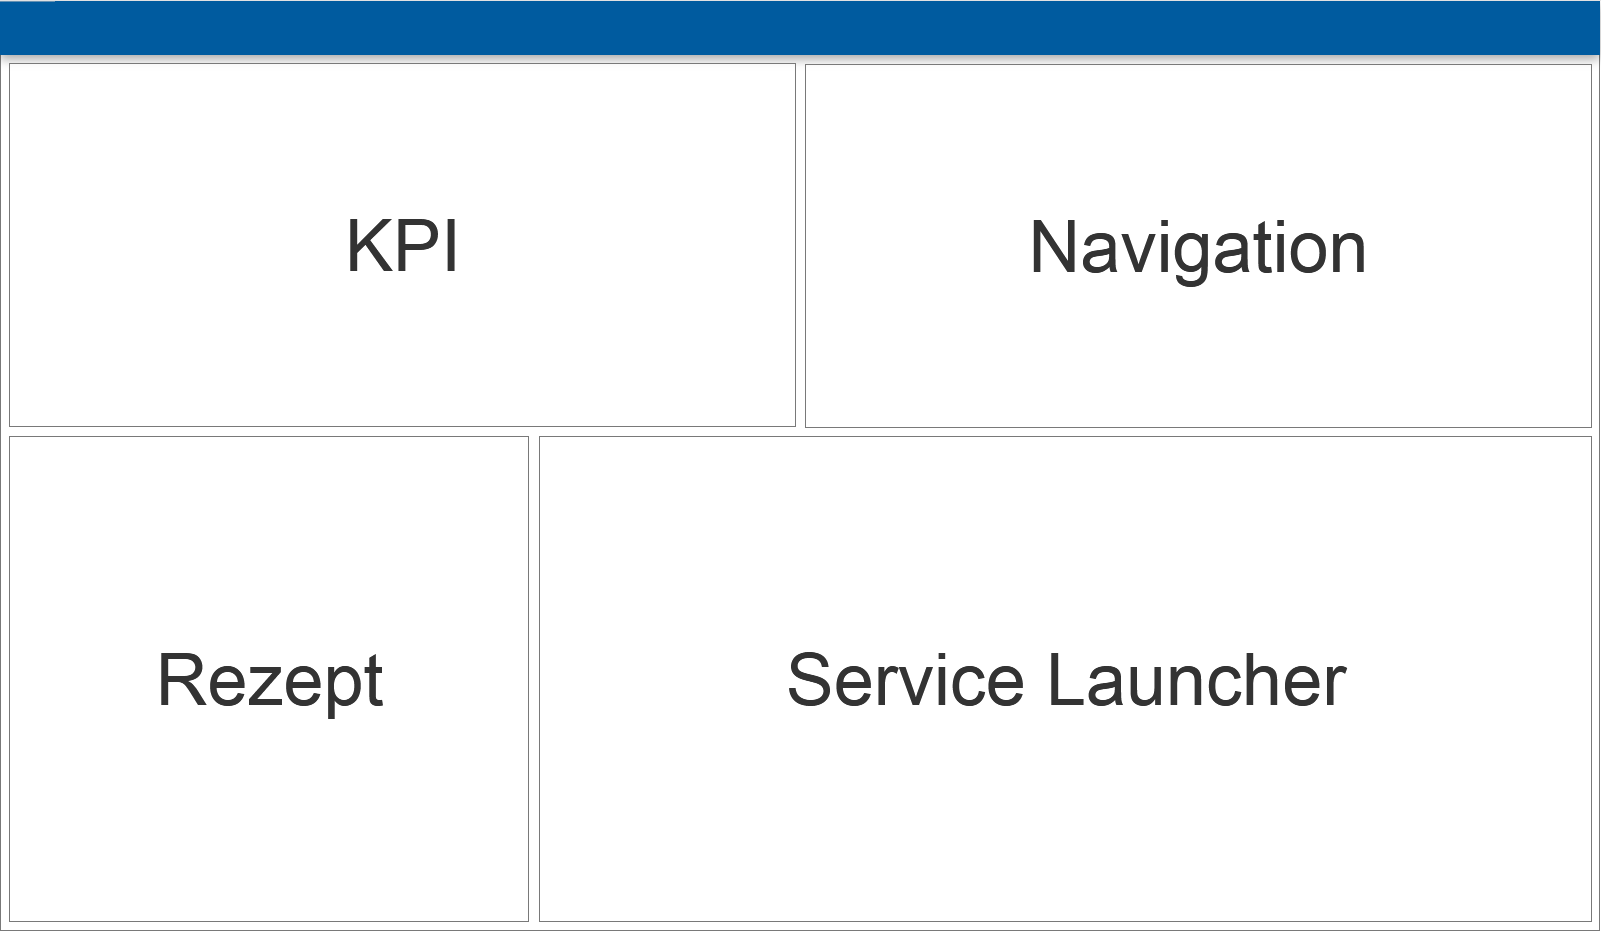
\includegraphics[scale=0.25]{DA_files/Bilder/Analyse/PFE-Bereiche.png}
\label{pic:Bereiche-PFE}
\caption{Die vier Bereiche der PFE}
\end{figure}

\begin{itemize}
\item \textbf{KPI:} Zeigt die KPI der einzelnen Module an.
\item \textbf{Navigation:} Zeigt eine Übersicht über die modulare Anlage an. Durch klicken auf einzelne Module gelangt man zu mehr Details.
\item \textbf{Rezept:} Zeigt das Rezept zur modularen Anlage an. Dieses ist aufgeteilt in Phases, Procedures und Steps (siehe Abschnitt \ref{2:Modulare-Anlagen}).
\item \textbf{Services / HMI:} Zeigt die Dienste der Module an. Diese beinhaltet den aktuellen Zustand und mögliche Zustandsübergänge, die aktuelle Strategie \todo{Fahrweise?} und die aktuelle Betriebsart. Des Weiteren können noch die vorhandenen Fahrweisenparameter angezeigt und eingestellt werden. Auf der letzten Ebene wird statt der Services das HMI des Moduls angezeigt.
\end{itemize}
Für eine besser Übersicht ist die PFE in vier Ebenen eingeteilt. Auf der obersten Ebene ist eine grobe Übersicht über die Anlage gegeben. Die unterste Ebene stellt die meisten Details dar. Tabelle \ref{tab:Ebenen-PFE} beschreibt, welche Informationen auf welcher Ebene dargestellt sind. Mittels der Navigation können die Ebenen gewechselt werden. \todo{Bilder der Ebenen in Anhang}
\begin{table}[htbp]
\centering
\begin{tabular}{p{1,7cm}|p{2,3cm}|p{2,2cm}|p{2,2cm}|p{2,3cm}|}
 & \textbf{Navigation} & \textbf{KPI} & \textbf{Rezept} & \textbf{Services / HMI} \\
\hline
\textbf{Ebene 1} & Shopfloor: Übersicht über alle vorhandenen Anlagen & & Phases für die angewählt Anlage & Alle Services der angewählten Anlage \\
\hline
\textbf{Ebene 2} & Subplant: Anzeige aller Module und deren Verbindungen & & Procedures & Alle Services der Anlage \\
\hline
\textbf{Ebene 3} & Modul & KPIs für das angewählte Modul & Procedures: Markierung des angewählten Moduls & Services des Moduls \\
\hline \textbf{Ebene 4} & Modul & & Procedures: Markierung des Moduls & Anzeige des HMI des Moduls \\
\hline
\end{tabular}
\label{tab:Ebenen-PFE}
\caption{Übersicht über die Ebenen in der Prozessführungsebene}
\end{table}


\section{Informationsbedarf}
Der Informationsbedarf orientiert sich maßgeblich an den Aufgaben und dem Nutzer. Wieso ist das so wichtig? \todo{weiter ausführen}

\subsection{Informationen nach Aufgabenbereich}
Neben den Informationen, die ein Modul zur Verfügung stellt und die bei Behebung einer Störung behilflich sein können, gibt es eine Reihe von weiteren interessanten Aspekten. Weitet man den Problembereich von einer reinen Instandhaltung auf Bereiche wie die Wirtschaftlichkeit aus, so werden ganz andere Informationen benötigt. Welche Funktionen auf welcher Ebene in einem Unternehmen automatisiert werden können und somit auch sinnvoll durch ein Assistenzsystem unterstützbar sind ist in \cite{Lauber1999} beschrieben. Hier ist auch der zeitliche Aspekt mit aufgeführt. Eine entsprechende Übersicht findet sich in Tabelle \ref{tab:Ebenen-Unternehmen}.
\begin{table}[htbp]
\centering
\caption{Ebenen in einem Unternehmen bei Führung technischer Prozesse}
\label{tab:Ebenen-Unternehmen}
\begin{tabular}{|p{0.2 \textwidth}|p{0.33 \textwidth}|p{0.33 \textwidth}|}
\hline
\textbf{Ebenen eines Unternehmens} & \textbf{zeitliche Anforderungen} & \textbf{Automatisierungs-funktionen} \\
\hline
Unternehmens-führung & Entscheidungen wirken sich langfristig aus (nach Monaten oder Jahren) & Kostenanalysen, statistische Auswertungen \\
\hline
Produktions-planung und Betriebsleitung & Änderungen werden nach Tagen, Wochen oder Monaten sichtbar & Betriebsablaufplanung, Kapazitätsoptimierung, Auswertung der Prozessergebnisse \\
\hline
Leitung technische Prozesse & Eingriffe wirken sich nach Stunden oder Minuten aus & Prozessüberwachung, An- und Abfahrten, Störungsbehandlung, Prozessführung, Prozesssicherung \\
\hline
Prozessgrößen & Auswirkungen sind nach Sekunden, Millisekunden oder gar Mikrosekunden sichtbar & Messen, Steuern, Stellen, Regeln, Verriegelungen, Not-Bedienen von Prozessgrößen, Abschalten, Schutz \\
\hline
\end{tabular}
\end{table}

\subsection{Informationsbedarf des Menschen}
\label{3:Informationsbedarf-Operator}
Stützt man sich bei der Ermittlung des Informationsbedarfs auf die individuellen Fähigkeiten und das vorhandene Wissen so ist eine entsprechende Analyse relativ komplex \todo{Nachweis?}. Insbesondere, wenn der Problemlöseprozess einen Lerneffekt haben soll. In der Literatur ist dies als Assistance Dilemma bezeichnet \todo{Zitat}. Wenn der Lerneffekt möglichst groß sein soll, wird Information über die Problemlösung und die Lösungsschritte zunächst zurück gehalten. Informationen werden interaktiv hinzugefügt, wenn sie benötigt werden. Die größte Herausforderung ist dabei die Kriterien festzulegen, wann Informationen gegeben und wann sie zurück gehalten werden\cite{Koedinger2007}.  Richey und Nokes-Malach \cite{Richey2013} empfehlen eine geringe Bereitstellung an hilfreichen Erklärungen bei Problemlöseaktivitäten, solange andere Ressourcen für den Lernprozess zur Verfügung stehen. Da diese Arbeit den Fokus auf eine geeignete Informationsaufbereitung legt, wird an dieser Stelle nicht weiter darauf eingegangen, wie der Lernerfolg des Menschen ideal unterstützt werden kann. Die Literatur \cite{Miller2005, Sauer2018} hebt hervor, dass Operator ein mittleres Level an Automatisierung bevorzugen. Auf diesem Level werden beim komplexen Problemlösen die meisten Varianten generiert. Bei keiner Unterstützung übersieht der Operator möglicherweise wichtige Aspekte. Bei einer hohen Automatisierung denkt der Operator nicht mehr über Alternativen nach und bestätigt den Vorschlag nur noch. \cite{Miller2005} Im Kontext des Modulaustausch könnte das System verschiedene Vorschläge liefern, die durch Vorschläge des Menschen ergänzt werden können.

In Abschnitt \ref{2:Unterscheidung-Probleme} ist bereits beschrieben, dass komplexe Probleme auf das Wesentliche reduziert werden müssen und häufig Informationsbeschaffung gefordert ist. In dieser Arbeit soll die Informationsbeschaffung unterstützt und die Übersichtlichkeit der Information zur Reduktion der Komplexität gewahrt werden.

Welche Informationen sind nun für den Modulbetreiber relevant, wenn ein Modul ausgetauscht werden muss?

Der sicherlich wichtigste Punkt ist die Kompatibilität. Passen die Anschlüsse zu den anderen Modulen der Anlage? Kann das Rezept weiterhin, wie konfiguriert gefahren werden oder sind Anpassungen notwendig? Um dies einschätzen zu können sind weitreichende Informationen über das Modul und die aktuelle Anlage notwendig. Diese umfassen
\begin{itemize}
\item \textbf{die Abmaße:} Passt das Modul von der Größe an die gleiche Stelle, wie das andere Modul?
\item \textbf{die Schnittstellen:} Ist das Modul mit den Schnittstellen der anderen Module kompatibel?
\item \textbf{das Rezept:} Welche Stellen im Rezept werden beeinflusst, wenn das Modul getauscht werden muss?
\item \textbf{die Services:} Welche Serviceabhängigkeiten bestehen zwischen dem Rest der Anlage und dem zu ersetzenden Modul?
\item \textbf{die Parameter:} Können die Parameter bei einem Austausch beibehalten werden oder müssen Anpassungen vorgenommen werden? Wenn Anpassungen vorgenommen werden müssen, welche Auswirkungen hat das auf den Prozess?
\end{itemize}

Ein Modulaustausch hat nicht nur auf der rein technischen Seite einen Einfluss. Ein Unternehmen muss noch viele weitere Faktoren berücksichtigen, um sich bei Alternativen für eine entscheiden zu können. Die Kriterien für die Auswahl werden durch die Ziele des Unternehmens bestimmt. Zur Unterstützung der Zielerreichung ist eine Verwendung von Kennzahlen möglich. Mit den Kennzahlen kann der aktuelle Zustand ermittelt und überwacht werden. Dabei muss auch festgelegt werden, welche Entscheidungsrelevanz die Kennzahl hat.  Bezogen auf den Modulaustausch könnten der Aufwand einer Rezeptänderung oder die Auswirkungen auf die Produktqualität relevant sein. Mit Sicht auf die Produktionsprozesse identifiziert Gottmann \cite{Gottmann2016} eine ganze Reihe von Faktoren, welche die Ziele beeinflussen können (siehe Bild \ref{pic:Produktionsprozesse-Zielgroessen} \todo{überarbeiten} analog zu \citep[50]{Gottmann2016}).
\begin{figure}[htb]
\centering
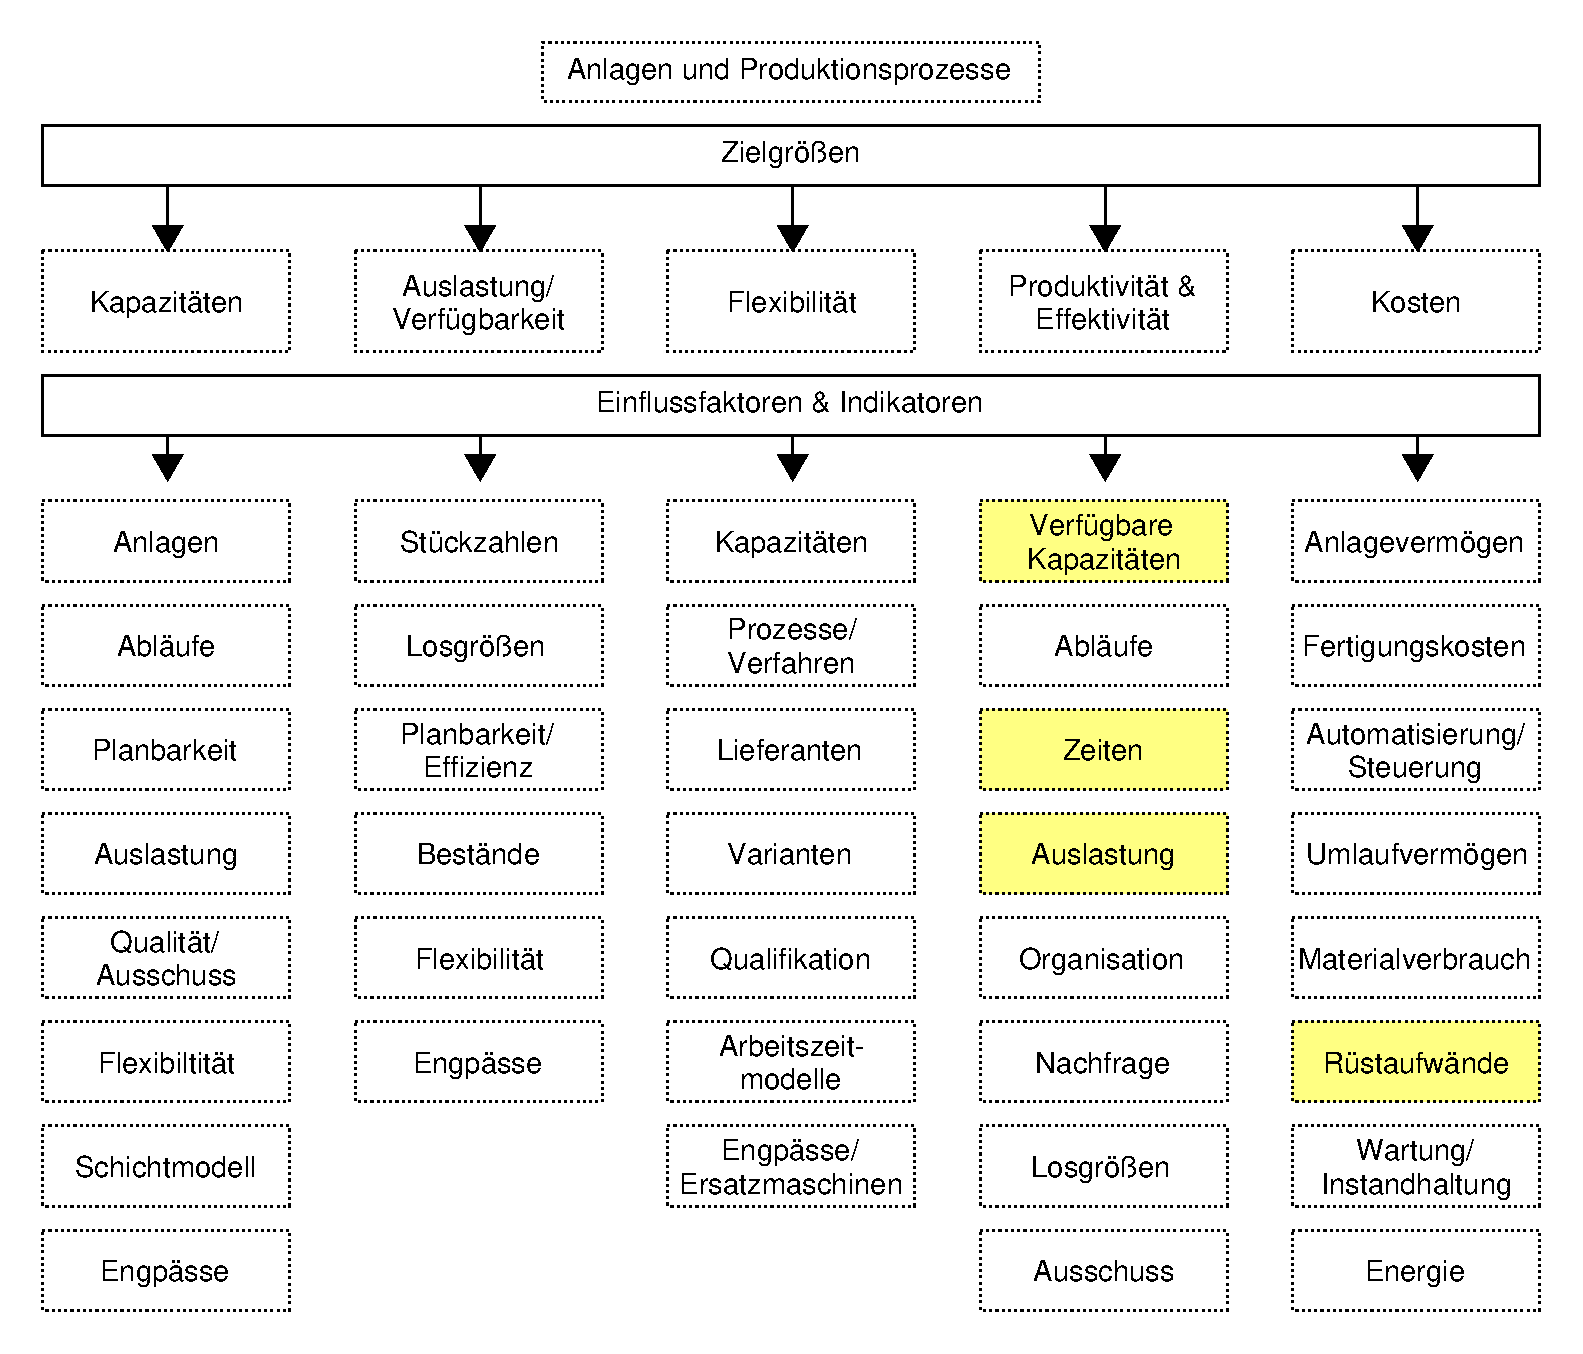
\includegraphics[scale=0.5]{DA_files/Bilder/Analyse/Produktionsprozesse-Zielgroessen.pdf}
\caption{Produktionsprozess: Zielgrößen und Einflussfaktoren}
\label{pic:Produktionsprozesse-Zielgroessen}
\end{figure}

In dieser Arbeiten werden nur einige wenige Einflussfaktoren berücksichtigt. Nicht für jedes Unternehmen und jede Ebene im Unternehmen ist jede Zielgröße und somit auch nicht jeder Einflussfaktor relevant. In dieser Arbeit wird der Fokus im Zuge des Modulaustauschs auf die Ebene der Produktionsplanung und Betriebsleitung gelegt. Auf dieser ist untere anderem die Kapazitätsoptimierung und damit das Ziel der Produktivität \& Effektivität relevant. Die Produktivität beschreibt, wie viel der verfügbaren Arbeitszeit zur Produktion verwendet wird. Steht aufgrund vieler Störungen in der Anlage die Produktion still, so ist die Produktivität gering. Bei einer hohen Effektivität werden die verfügbaren Ressourcen ideal genutzt. Dies kann beispielsweise die Zeit sein, die eine Reparatur in Anspruch nimmt. Folgende Einflussfaktoren sollen im weiteren Verlauf der Arbeit berücksichtigt werden:
\begin{itemize}
\item \textbf{Zeiten:} Wie viel Stillstandzeit verursacht der Modulaustausch?
\item \textbf{Auslastung:} Besteht die Möglichkeit vor zu produzieren?
\item \textbf{Rüstaufwände:} Was muss alles im Rezept verändert werden? Welche Zeit nimmt das in Anspruch?
\item \textbf{Verfügbare Kapazitäten:} Wie viele Mitarbeiter stehen für den Modultausch zur Verfügung? 
\end{itemize}

\section{Informationsanpassung}
Die Individualisierung von Software bietet die Möglichkeit eine Vielzahl von Nutzer und Aufgaben zu unterstützen. Individualisierung dient der Modifizierung von Interaktion und Informationsdarstellung, um unter anderem den Fähigkeiten und Bedürfnissen jedes Benutzers gerecht zu werden. Ebenso ist auch die Anpassung an das zu lösende Problem nicht zu unterschätzen. Je nach Zielstellung müssen andere Informationen hervor gehoben werden.

\subsection{Individualisierung für den Menschen}
Individualisierung für den Nutzer kann vielschichtig sein. In Abschnitt \ref{2:Individualisierung} sind bereits einige Aspekte für Individualisierung thematisiert. Zu Berücksichtigen sind bei Sicht auf den Nutzer unter anderem:
\begin{itemize}
\item \textbf{Fähigkeiten:} Welche besonderen Fähigkeiten hat der Nutzer? Wie können diese in Kollaboration mit der Assistenz sinnvoll genutzt werden?
\item \textbf{Vorwissen:} Was weiß der Nutzer über die modulare Anlage?
\item \textbf{Position:} Welche Aufgabe hat der Nutzer? Auf welcher Ebene des Unternehmens arbeitet dieser? Welche Informationen sind für ihn besonders relevant?
\end{itemize}
Soll jeder Nutzer des Assistenzsystemes individuell anhand seiner kognitiven Leistung unterstützt werden, so ist herauszufinden, ob der Mensch aktuell mit der Aufgabe über- oder unterfordert ist. Eine Möglichkeit ist die Art und Weise der Interaktion auszuwerten und entsprechende Anpassungen vorzunehmen. Wie bereits in Abschnitt \ref{2:Adaptive-Systeme} beschrieben, sind dabei viele Einflussfaktoren zu berücksichtigen. Eine Auswertung dieser sprengt leider den Rahmen der Arbeit. \todo{Was schaue ich mir an?}

\subsection{Anpassung an die Aufgabe}
\label{3:Anpassung-Aufgabe}
Wie schon in Abschnitt \ref{2:Unterscheidung-Probleme} beschrieben, lassen sich Probleme anhand verschiedener Aspekte unterscheiden. So ist zum Beispiel der Zeitdruck ein wichtiger Aspekt. Bei zeitkritischen Problemen muss möglichst schnell eine gute Lösung gefunden werden. Ist das Problem nicht zeitkritisch, können in Ruhe alle zur Verfügung stehenden Informationen in den Problemlöseprozess mit einbezogen werden. So kann bei einem zeitkritischen Problem ein höherer Automatisierungsgrad gefordert sein. Um dennoch dem Menschen seine Kompetenzen nicht abzusprechen, ist es möglich bei Problemen, die eher langfristig sind und die eine höhere kognitive Aktivität erfordern, eine geringere Autonomiestufe anzuwenden. Dadurch kann der Mensch sich Wissen über den Prozess aneignen und seine Kompetenzen ausbauen.

Angenommen der Nutzer hat viel Zeit sich mit dem Problem zu beschäftigen, so müssen sich die bereitgestellten Informationen auch am Probleminhalt orientieren. Der Austausch eines Moduls bedarf einer Übersicht der Kompatibilität mit der bestehenden Anlage und dem Rezept. Entsteht ein Problem aufgrund eines fehlgeschlagenen Services, so ist das zugehörige Equipment und die eingestellten Parameter relevant. Durch die Aufbereitung dieser Informationen und deren Abhängigkeiten kann schrittweise die Ursache gefunden werden.

Ein ebenfalls wichtiger Aspekt, der schon in Abschnitt \ref{3:Informationsbedarf-Operator} thematisiert wurde, ist die Zielsetzung des Unternehmens. Diese kann sehr unterschiedlich sein, was sich maßgeblich auf die Informationsbereitstellung auswirkt. Ist beispielsweise die Stillstandzeit der Anlage besonders relevant, so sollten diese Informationen hervor gehoben werden. In einem anderen Kontext kann aufgrund von Personalmangel der Rüstaufwand eine höhere Priorität bekommen.

\section{Interaktionsmechaniken}
Im Kontext dieser Arbeit wird das Problemlösen betrachtet. Problemlösen heißt in diesem Fall aus mehreren Alternativen die geeignetste für das Erreichen des festgelegten Ziels auszuwählen. In Abschnitt \ref{2:Assistenzsysteme} sind verschiedene Interaktionsmechaniken beschrieben. Um diese geeignet bewerten zu können ist zunächst eine Begutachtung des Arbeitsumfelds und der Aufgaben notwendig.

Da sich das Problemlösen im Rahmen dieser Arbeit nicht auf das Beheben von Störungen bezieht, kann angenommen werden, dass die Hände nicht für andere Aufgaben frei sein müssen. Zudem ist eine geeignete Darstellung von Zusammenhängen notwendig, welches eine entsprechende Displaygröße voraussetzt. Diese Zusammenhänge müssen durch den Menschen entsprechend interpretiert werden, damit dieser mit dem System interagieren kann. Es muss dazu die Möglichkeit gegeben sein selbst Vorschläge für die Lösung des Problems zu liefern. Das setzt vielfältige Eingabemöglichkeiten voraus. \todo{spezifizieren!}

Daraus abgeleitet wird für die Umsetzung des Assistenzsystem ein Tablet verwendet. Diese ist groß genug, um alle notwendigen Informationen anzuzeigen. Es ist flexibel genug, wenn für den Problemlöseprozess Informationen benötigt werden, die nur durch Begutachtung der Anlage erlangt werden können. Zudem bietet die Kamera die Möglichkeit Augumented Reality zu verwenden oder das Mikrofon die Möglichkeit Spracheingaben zu tätigen.



\section{Anforderungen an das Assistenzsystem}

\subsection{Funktionale Anforderungen}

\subsubsection*{Unterstützung der Problemidentifikation}
\begin{itemize}
\item[PI 1] Der Nutzer soll durch die Problemlösung begleitet werden können, indem...
	\begin{itemize}
	\item[PI 1.1] ...er das Problem beschreiben kann.
	\item [PI 1.2] ...er Ziele definieren kann.
	\item[PI 1.3] ...ihm alle Informationen über die aktuelle Situation zur Verfügung stehen.
	\end{itemize}
\item[PI 2] Das Assistenzsystem soll den Nutzer bei der Problemidentifikation unterstützen.
\item[PI 3] Dem Nutzer soll es möglich sein Ziele hinzuzufügen.
\item[PI 4] Dem Nutzer soll der Auslöser des Problems und der zugehörige Problembereich mitgeteilt werden.
\end{itemize}

\subsubsection*{Unterstützung bei der Problemlösung}
\begin{itemize}
\item[PL 1] Das Assistenzsystem soll mögliche Lösungen vorschlagen.
	\begin{itemize}
	\item[PL 1.1] Diese sollen sich an den festgelegten Zielen orientieren.
	\end{itemize}
\item[PL 2] Der Nutzer soll mögliche Lösungen vorschlagen können.
\item[PL 3] Die Lösungen sollen vergleichbar sein, indem...
	\begin{itemize}
	\item[PL 3.1] ...die Auswirkungen auf die Anlage/ den Prozess dargestellt werden.
	\item[PL 3.2] ...
	\end{itemize}
\item[PL 3] Die Lösungen sollen bewertbar sein.
\end{itemize}

\subsubsection*{Kluster von Problemen}
\begin{itemize}
\item[KP 1] Es sollen mehrere Probleme gleichzeitig bearbeitet werden können.
\item[KP 2] Die Probleme sollen sich sortieren lassen.
\item[KP 3] Die Probleme sollen mit Merkmalen versehen werden können.
	\begin{itemize}
	\item[KP 3.1] Zeit: Problem ist zeitkritisch und muss schnell gelöst werden oder es ist viel Zeit vorhanden, um über eine mögliche Lösung nachzudenken.
	\item[KP 3.2] Komplexität: Wird die Problemlösung durch viele oder wenige Größen beeinflusst?
	\item[KP 3.3] Aufwand: 
	\end{itemize}
\end{itemize}

\subsection{Nichtfunktionale Anforderungen}
\begin{itemize}
\item[NA 1] Die Bedienung soll über ein Tablet realisiert werden.
\end{itemize}

%%%%%%%%%%%%%%%%%%%%%%%%%%%%%%%%%%%%%%%%%%%%%%%%%%%%
\chapter{Konzept}
\label{sec:Konzept}
%%%%%%%%%%%%%%%%%%%%%%%%%%%%%%%%%%%%%%%%%%%%%%%%%%%%
In der Analyse wurde herausgearbeitet, welche Aspekte bei der Entwicklung des Assistenzsystems für die modularen Anlagen berücksichtigt werden müssen. Die vielschichtigen Faktoren werden nun ins Konzept mit einbezogen. Dazu wird zunächst mit dem konzeptionellen Design herausgearbeitet, welche Funktionen konkret umgesetzt werden müssen und wie Nutzer und Assistenz miteinander interagieren. Darauf aufbauend erfolgt der Entwurf eines physikalischen Designs. In diesem wird ein Vorschlag geliefert, wie ein System zur Problemlösung aussehen kann.

Wo kommt das mit dem physikalischen und konzeptionellem Design her? \todo{Quelle ergänzen}

\section{Konzeptuelles Design}
\todo{Einleitung?}
\begin{figure}[htbp]
\centering
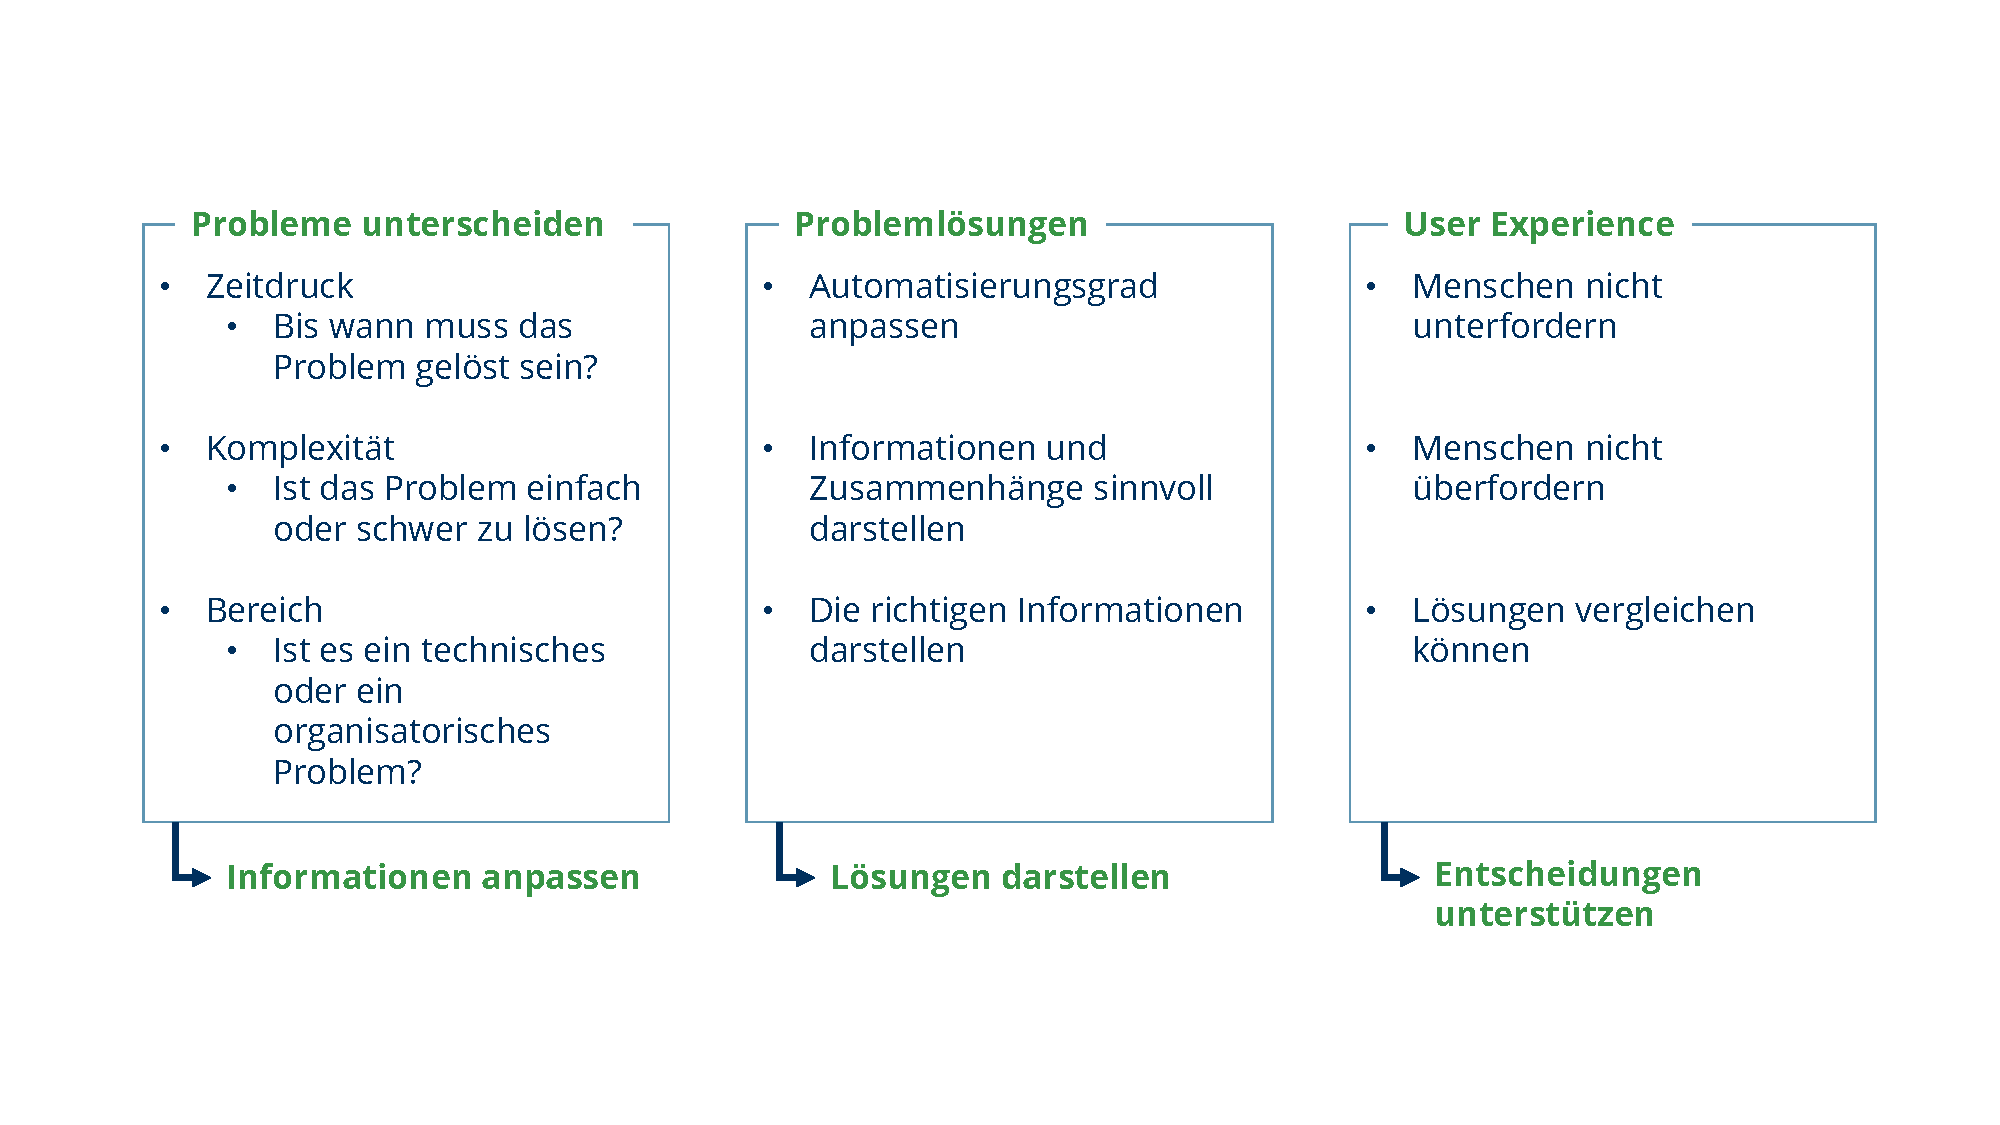
\includegraphics[scale=0.45]{DA_files/Bilder/Konzept/Nutzer-unterstuetzen.pdf}
\caption{Aspekte des Assistenzsystems}
\label{pic:Nutzer-Unterstuetzen}
\end{figure}
\\ \\
In Abschnitt \ref{2:Unterscheidung-Probleme} ist bereits aufgeführt, dass sich \textbf{Probleme unterscheiden}. Die Informationen sollen sich entsprechend dem Zeitdruck, der Komplexität des Problems und dem umfassenden Bereich automatisch anpassen. Dadurch soll sowohl eine Unterforderung, als auch eine Überforderung des Menschen verhindert werden.

Die \textbf{Lösungen für das Problem} sollen sinnvoll dargestellt werden. Dabei wird der Autonomiegrad anhand des Zeitdrucks angepasst. Die Menge an dargestellten Informationen und deren Zusammenhänge orientieren sich an der Komplexität des Problems. Die Komplexität des Problems lässt sich aus der Menge an Zusammenhängen ableiten. Deshalb ist es umso wichtiger diese strukturiert und klar darzustellen. Abhängig vom Bereich des Problems sind die richtigen Informationen darzustellen.

Mit einer guten \textbf{User Experience} soll die Entscheidung des Menschen unterstützt werden. Dieser soll mittels geeignetem Autonomiegrad nicht unterfordert werden. Durch die angemessene Darstellung der Informationen ist eine Überforderung zu vermeiden. Die Darstellung der Informationen hängt auch mit der Vergleichbarkeit der Lösungen zusammen. Gibt es mehrere Lösungen, so muss der Nutzer Unterschiede gut erkennen können, um eine geeignete Entscheidung zu treffen.
\\ \\
Wie kann nun der Nutzer durch den Problemlöseprozess begleitet werden? In Abschnitt \ref{2:Phasen-Problemloesen} sind die Phasen des Problemlösens beschrieben. Angelehnt daran wird folgender Ablauf mit entsprechender Unterstützung durch das Assistenzsystem vorgesehen (siehe Bild \ref{pic:Konzeptidee}).
\begin{figure}[htbp]
\centering
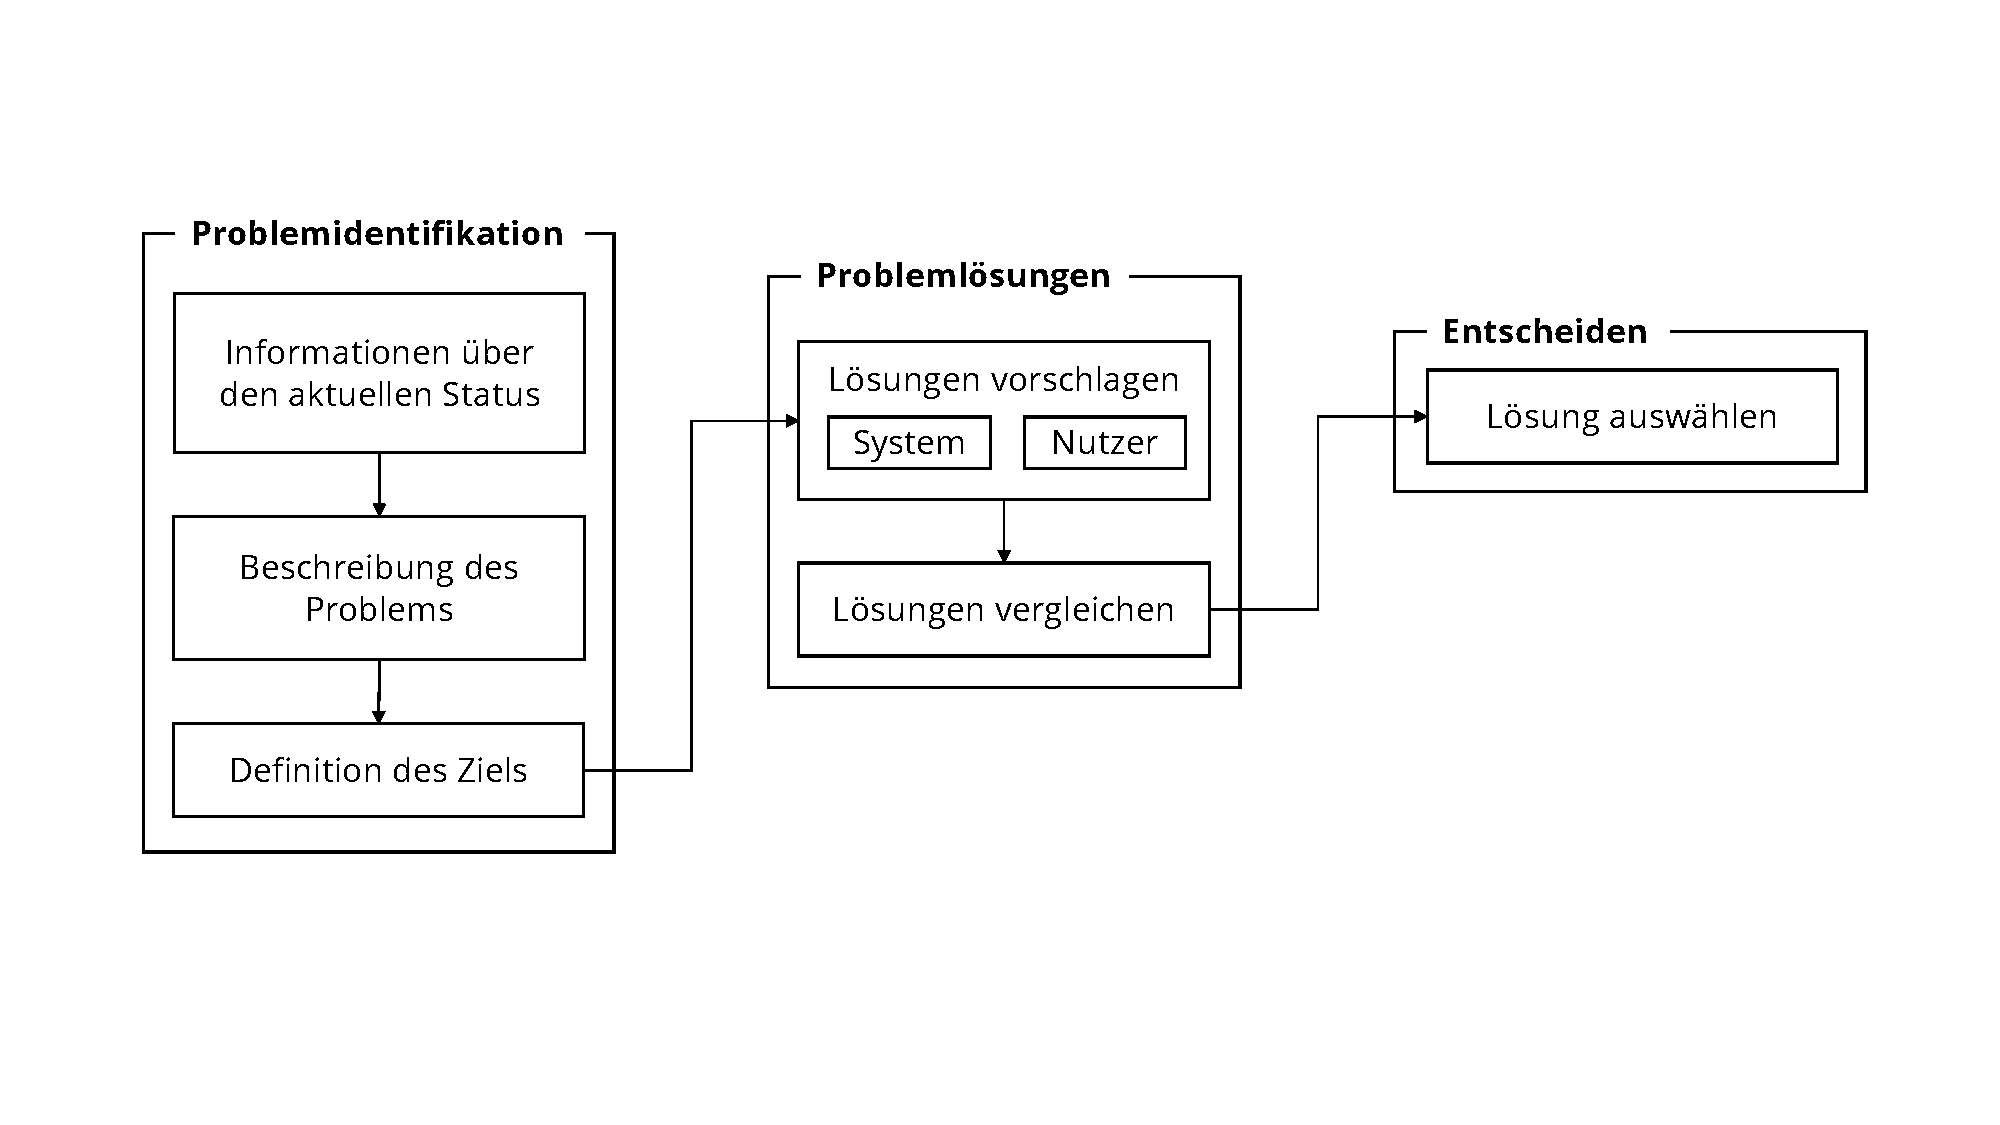
\includegraphics[scale=0.45]{DA_files/Bilder/Konzept/Konzeptidee.pdf}
\caption{Die Schritte des Problemlöseprozess}
\label{pic:Konzeptidee}
\end{figure}

Zunächst muss das Problem identifiziert werden. Dazu stehen dem Nutzer alle Informationen über den aktuellen Status der modularen Anlage zur Verfügung. Durch Meldungen, Warnungen und Alarme können Probleme vom System ausgelöst werden. Weiterführend ist es denkbar, dass auch der Nutzer ein Problem definiert. Ist das Problem identifiziert, so muss das Ziel definiert werden. Im Fall eines zu wartenden Moduls kann z.B. ein maximaler Produktionsausfall angegeben werden.

Ist das Problem identifiziert und das Ziel definiert, so müssen die möglichen Lösungen betrachtet werden. Lösungen können sowohl vom System, als auch vom Nutzer vorgeschlagen werden. Nach Bestimmung der Lösungen erfolgt ein Vergleich dieser.

Die Entscheidung für eine entsprechende Lösung wird mittels einer geeignete Darstellung durch das Assistenzsystem unterstützt. Wie dies aussehen kann ist in Abschnitt \ref{4:pD-Loesungen} dargestellt.

\subsection{Funktionen}
\todo{einleitenden Text schreiben}
Wie kann nun der oben beschriebene Problemlöseprozess unterstützt werden? Zunächst muss der Nutzer einen Überblick über den aktuellen Status erhalten. Taucht ein neues Problem auf so interagieren Nutzer und Assistent bis eine geeignete Lösung gefunden wird. Mehr dazu in Abschnitt \ref{4:Kollaboration}.

\subsubsection*{Aktueller Status}
Der aktuelle Status kann über die PFE abgelesen werden. Diese gibt einen Überblick über die aktuelle Verschaltung der Module, das Rezept, die Key Performace Indicator (KPIs) und die Services. Auch eine Übersicht über das Anlagenequipment eines jeden Moduls ist vorhanden. Die notwendigen Meldungen, Warnungen und Alarme werden derzeit nicht angezeigt. Durch die Integration dieser kann der Nutzer bei der Problemidentifikation unterstützt werden. Tritt beispielsweise eine Meldung auf, hat der Nutzer die Möglichkeit dieses als Problem aufzunehmen und nach Lösungen zu suchen.

\subsubsection*{Neues Problem}
Welche Rahmenbedingungen sind für die Charakterisierung eines Problems relevant? In der Analyse (ref) wird sowohl auf die technischen, als auch die wirtschaftlichen Ziele verwiesen. Im Kontext eines produzierenden Unternehmens ist die Wirtschaftlichkeit eine wichtige ökonomische Zielgröße \cite{} (Bloech-Einführung in die Produktion). Dem Nutzer wird aus diesem Grund die Möglichkeit gegeben relevante Ziele hinzuzufügen und genauer zu spezifizieren. Welche dies genau sein können ist von dem Unternehmen und dem Problem abhängig.

Neben der Definition der Ziele, ist es dem Nutzer möglich eine Übersicht über den Problembereich zu erhalten. Dazu markiert das Assistenzsystem zunächst den Bereich in dem das Problem ausgelöst wurde und die zugehörigen Komponenten. Betrifft der Bereich ein bestimmtes Modul, dann werden die zugehörigen Services und der zugehörige Bereich im Rezept markiert. Betrifft der Bereich einen Service, sind die Parameterabhängigkeiten und das zugehörige Equipment relevant. Ausgehend von dem markierten Bereich und geleitet durch die Ziele können Lösungen gefunden werden.

\subsubsection*{Lösungen suchen}
Wie die konkrete Lösung für ein Problem aussieht ist nicht vorherbestimmt. Das Assistenzsystem kann anhand der definierten Ziele Vorschläge liefern. Diese können durch den Nutzer angepasst und bewertet werden. Hier ist der Mensch klar im Vorteil, da dieser Optionen abwägen kann. Des Weiteren hat der Nutzer die Möglichkeit selber nach Lösungen zu suchen. Ihm stehen dazu alle Informationen über die Anlage zur Verfügung. Das Assistenzsystem markiert die Veränderungen, die durch die Lösungen entstehen. Dadurch kann der Nutzer den Aufwand abschätzen und bewerten, ob die Lösung gut oder schlecht ist.

\subsubsection*{Lösungen vergleichen}
In vielen Fällen gibt es nicht nur eine richtige Lösung, sondern mehrere Lösungsmöglichkeiten, die gegeneinander abgewogen werden müssen. Dem Nutzer werden dazu die Unterschiede zwischen den Lösungen aufgezeigt. Diese können rein zahlenmäßig sein, wie entstehende Kosten oder die Länge des Stillstands. Es ist jedoch auch möglich, dass sich Lösungen strukturell unterscheiden, z.B. anhand der zur Verfügung gestellten Dienste. Durch einen Vergleich der Lösungen kann der Nutzer eine Entscheidung treffen und damit den Problemlöseprozess abschließen.

\subsubsection*{Klustern von Problemen}
Mit dem Assistenzsystem soll es möglich sein mehrere Probleme gleichzeitig zu bearbeiten, wenn das aktuelle Problem nicht sofort gelöst werden muss. Der Nutzer hat zu jedem Zeitpunkt der Problemlösung die Möglichkeit das Problem zu wechseln. Für die Einschätzung \todo{weiter ausführen}

\subsection{Anpassungen an den Problembereich}
Da sich sowohl Probleme, als auch Lösungen von Fall zu Fall unterscheiden, müssen dementsprechend Anpassungen vorgenommen werden. In Abschnitt \ref{3:Anpassung-Aufgabe} ist bereits erwähnt, dass sich die Informationen an das Problem und die Ziele anpassen sollten. Im Zuge dessen sind vor allem die gegenseitigen Abhängigkeiten relevant, auf die im weiteren Verlauf näher eingegangen wird. Damit sich das Assistenzsystem anpassen kann muss identifiziert werden, wo das Problem entstanden ist. Es lassen sich folgende Fälle unterscheiden:
\begin{itemize}
\item \textbf{Modul:} Das gesamte Modul hat ein Problem verursacht.
\item \textbf{Service:} Ein Service hat eine Warnung oder Alarm ausgelöst.
\item \textbf{Rezept:} Das Rezept ist an einer bestimmten Stelle hängen geblieben und kann nicht weiter abgearbeitet werden.
\item \textbf{KPI:} Die KPI weisen Unregelmäßigkeiten auf oder erreichen vorher definierte Grenzwerte.
\end{itemize}

\subsubsection*{Modul}
Ein einzelnes Modul ist sehr eigenständig, da es grundsätzlich auch alleine betrieben werden kann. In der Navigation der PFE ist ersichtlich mit welchen anderen Modulen es verbunden ist. Um eine Problemlösung auf Modulebene zu unterstützen ist es notwendig die zugehörigen Services und den Bereich im Rezept zu markieren. Dadurch kann der Nutzer die Abhängigkeiten erkennen. 

\subsubsection*{Services}
Die Services weisen eine Vielzahl an Abhängigkeiten auf. So kann ein Service direkt mit anderen Services gekoppelt sein (vgl. Abschnitt \ref{2:Modulare-Anlagen}) oder durch Parameter eines anderen Services gestartet werden. Diese Kopplung ist auch modulübergreifend möglich. Löst nun ein Service ein Problem aus, werden die abhängigen Services markiert. Dies erleichtert dem Nutzer die Eingrenzung des Problembereichs. Bei der Suche nach Lösungen, muss es dem Nutzer möglich sein alle Optionen in Erwägung zu ziehen. Dafür steht dem Nutzer auch die Information über das zugehörige Equipment der Services zur Verfügung, sofern diese vom Modulhersteller zur Verfügung gestellt werden.

\subsubsection*{Rezept}
Wird das Rezept automatisch ausgeführt besteht die Möglichkeit, dass dieses aufgrund eines Fehlers nicht vollständig ausgeführt werden kann. In so einem Fall wird dem Nutzer angezeigt an welcher Stelle das Rezept abgebrochen wurde und welche Services zugehörig sind. Ausgehend von der Position im Rezept können die notwendigen Bedingungen überprüft und mögliche Ursachen in Erwägung gezogen werden. Ist die Ursache identifiziert können mit Hilfe des Assistenzsystems Lösungen gefunden werden. So ist es dem Nutzer möglich Veränderung an der entsprechenden Stelle im Rezept vorzunehmen. Diese können dann vom Assistenzsysteme virtuell geprüft werden. Auf diese Weise entsteht eine kollaborative Problemlösung.  

\subsubsection*{KPI}
Die Key Performace Indicator beinhalten Kennzahlen zu dem Prozess im Modul. Treten Unregelmäßigkeiten auf oder überschreiten die KPIs vorher festgelegte Grenzwerte so kann dadurch ein Problem ausgelöst werden. Aktuell liegen keine beispielhaften KPIs vor. Denkbar ist es, dass zu den KPI zugehörige Module und Services markiert werden.

\subsection{Finden von Lösungen}
Das Assistenzsystem sucht anhand der Problembeschreibung und der definierten Ziele die Lösungen. Wie diese Suche konkret durchgeführt wird, soll hier nicht näher betrachtet werden. Denkbar sind Möglichkeiten des Machine Learnings, Case Base Reasoning oder  \todo{Möglichkeiten auflisten}

Ob bereits existierende Systeme, wie der PEA-Manager von Jan Funke \cite{Funke2018} verwendet werden können, ist in weiteren Arbeiten zu analysieren. \todo{weitere Systeme suchen}

\subsection{Kollaboration zwischen Nutzer und Assistenz}
\label{4:Kollaboration}
Für die Kollaboration zwischen Nutzer und Assistenz ist eine Interaktionsplattform notwendig, die einen Austausch ermöglicht. Diese bietet dem Nutzer die Möglichkeit Eingaben zu tätigen und der Assistenz die Möglichkeit Daten anzuzeigen.

\subsubsection*{Nutzer}
Der Nutzer arbeitet mit den Informationen, die ihm durch die Interaktionsplattform zur Verfügung gestellt werden. Wenn eine Meldung auftritt, dann entscheidet er, ob das Problem bearbeitet wird oder nicht. Ebenso entscheidet der Nutzer, welche Ziele für das Problem berücksichtigt werden sollen. Welche Entscheidungen der Nutzer trifft, ist in Abbildung \ref{pic:Kollaboration-Nutzer} verdeutlicht.
\begin{figure}[htbp]
\centering
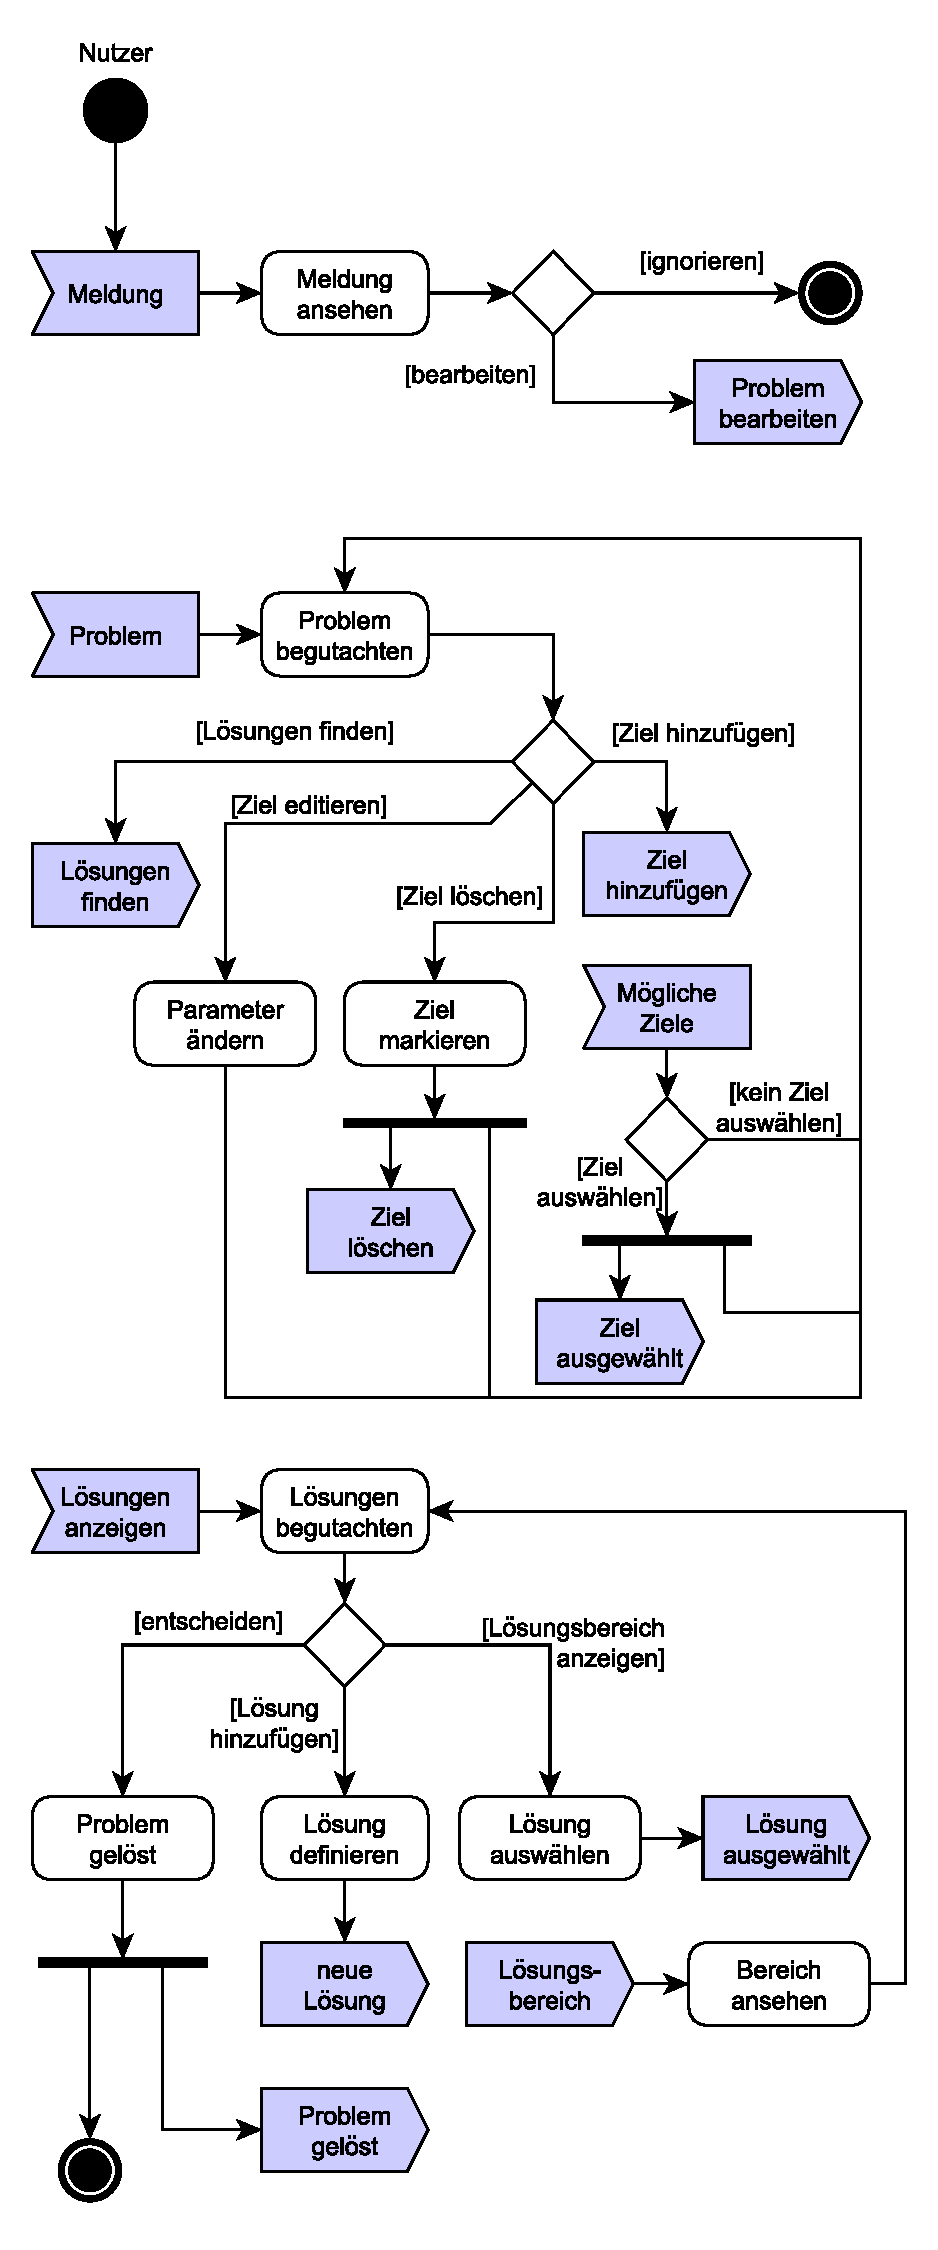
\includegraphics[scale=0.5]{Da_files/UML/Konzept/Aktivitaetsdiagramm-Nutzer.pdf}
\caption{Aktivitätsdiagramm: Kollaboration Nutzer}
\label{pic:Kollaboration-Nutzer}
\end{figure}

\subsubsection*{Interaktionsplattform}
Die Interaktionsplattform stellt die Verbindung zwischen Nutzer und Assistenzsystem dar. Die entsprechenden Verknüpfungen und Aktionen der Interationsplattform sind in Abbildung \ref{pic:Kollaboration-Interaktionsplattform} dargestellt.

\begin{figure}[htbp]
\centering
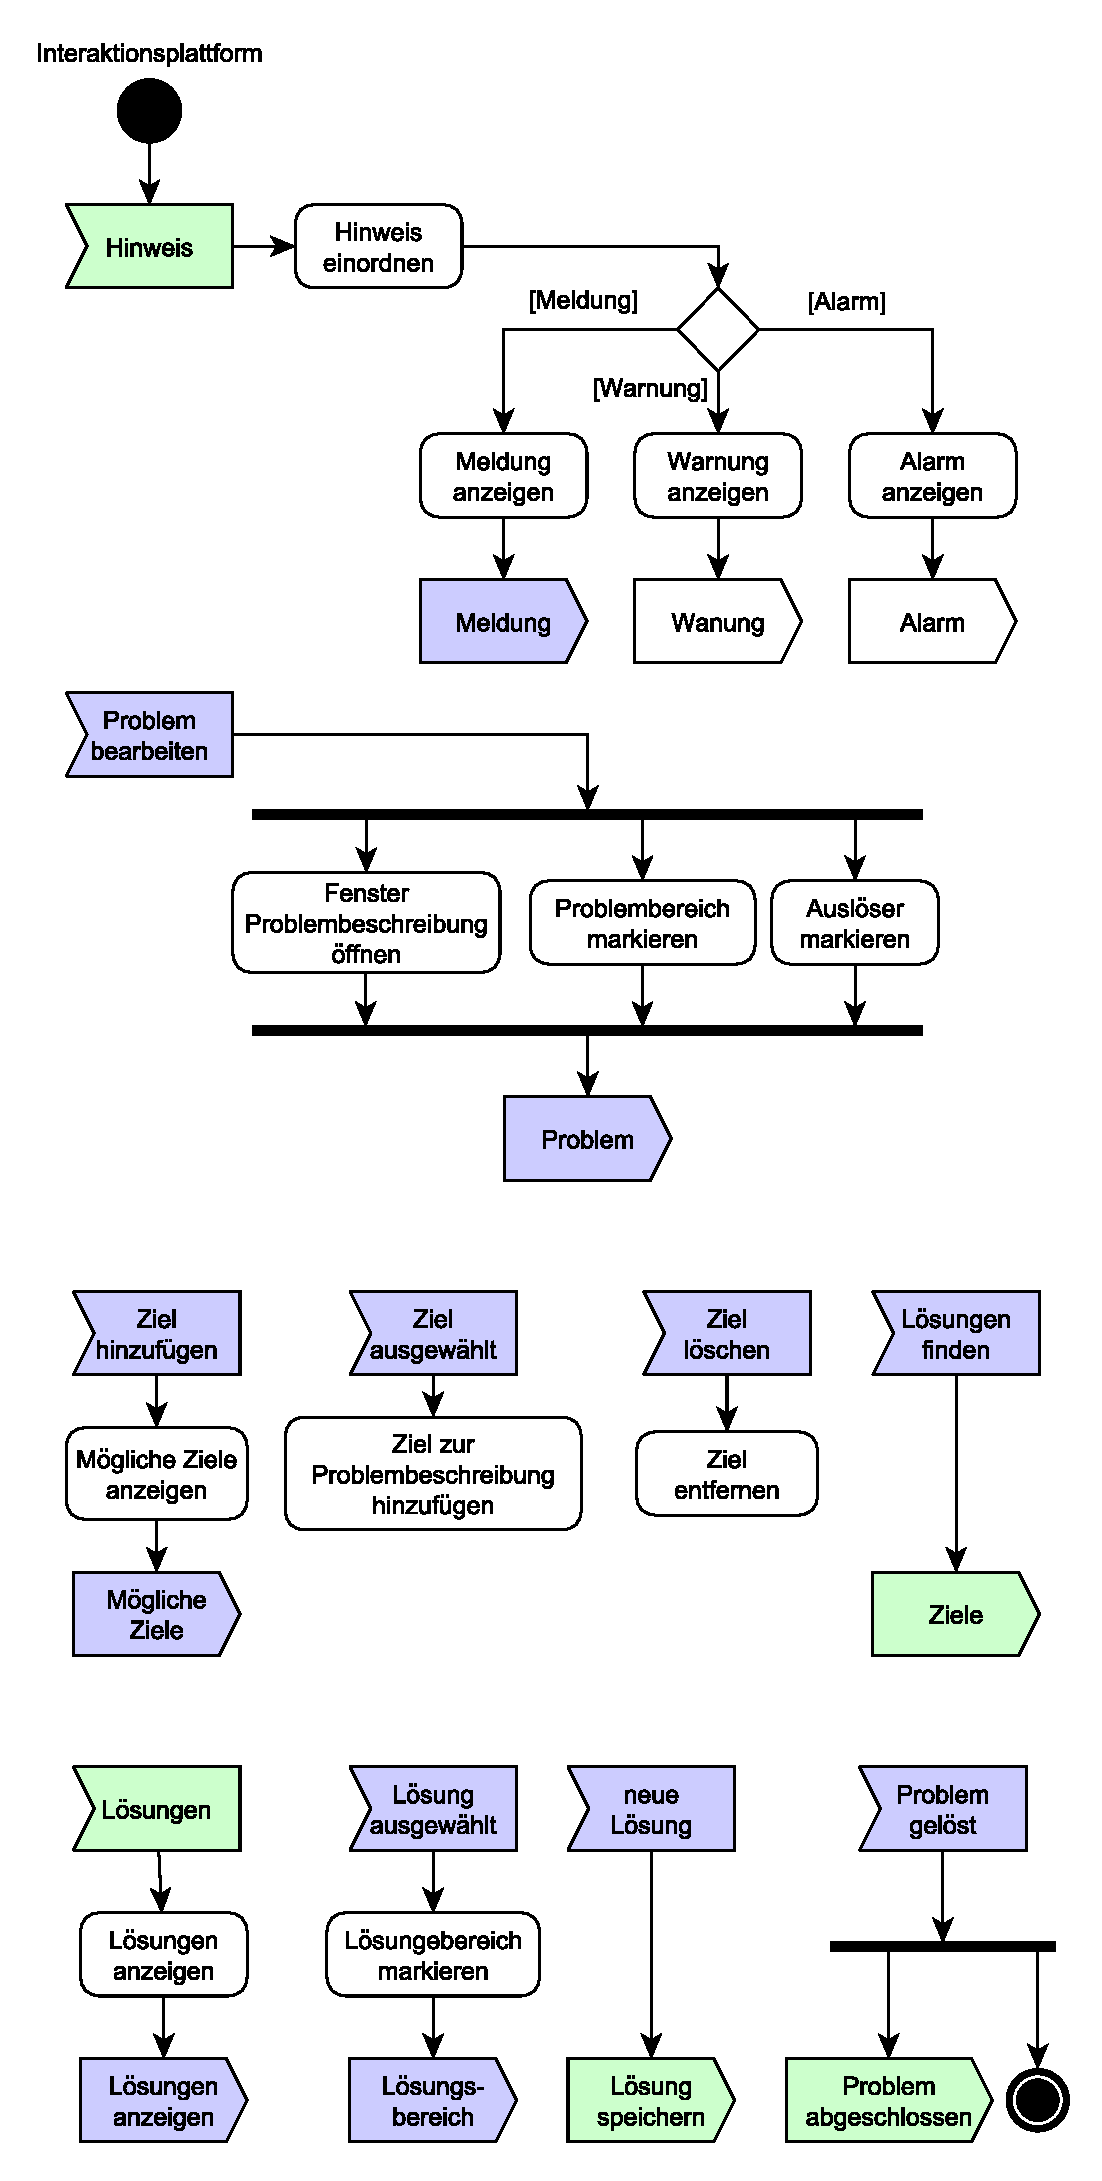
\includegraphics[scale=0.5]{DA_files/UML/Konzept/Aktivitaetsdiagramm-Interaktionsplattform.pdf}
\caption{Aktivitätsdiagramm: Kollaboration Interaktionsplattform}
\label{pic:Kollaboration-Interaktionsplattform}
\end{figure}

\subsubsection*{Assistenzsystem}
Das Assistenzsystem verarbeitet alle zur Verfügung stehenden Informationen und schickt entsprechende Signale an die Interaktionsplattform (siehe Abbildung \ref{pic:Kollaboration-Assistenzsystem}).
\begin{figure}[htbp]
\centering
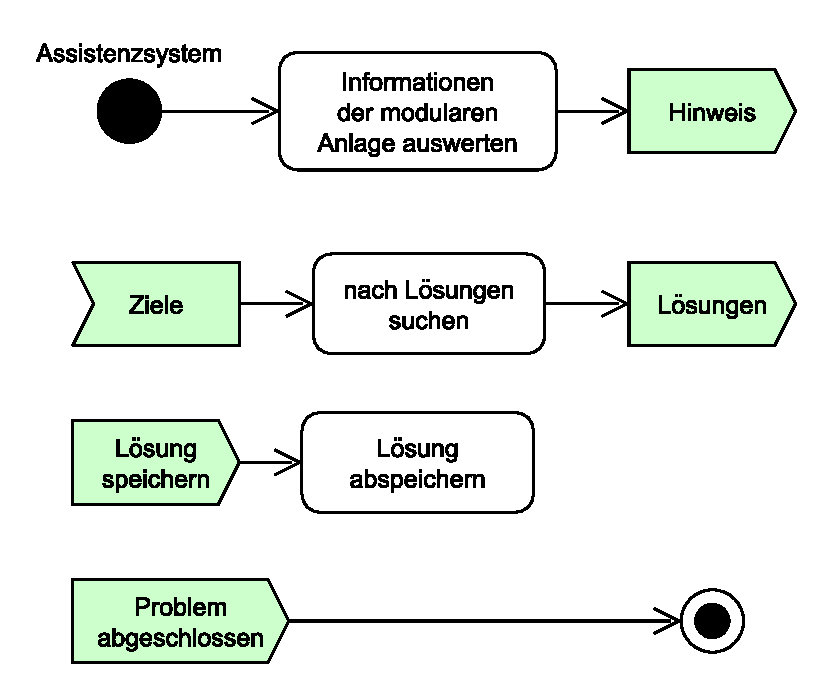
\includegraphics[scale=0.5]{DA_files/UML/Konzept/Aktivitaetsdiagramm-Assistenz.pdf}
\caption{Aktivitätsdiagramm: Kollaboration Assistenzsystem}
\label{pic:Kollaboration-Assistenzsystem}
\end{figure}

\section{Physikalisches Design}
\label{4:Physikalische-Design}
Ausgehend vom konzeptuellen Design wird das physikalische Design entworfen. Es beschreibt die konkrete Darstellung der Funktionen und Informationen. Das Design baut auf der bereits existierenden PFE auf und erweitert diese. Grundlage bietet das Material Design \cite{MaterialDesign} von Google. Zur klaren Abgrenzung von Assistenzsystem und PFE wird auch das Farbschema erweitert. Das Assistenzsystem bedient sich an Grüntönen, die mittels des Color Tools \cite{} ausgewählt wurden.

\subsection{Prozessführungsebene}
In der bereits existierenden Prozessführungsebene ist der aktuelle Status sichtbar. In Bild \ref{pic:pD-PFE} ist die PFE um eine Meldung erweitert. Über den Button \textbf{Problem bearbeiten} gelangt man zur Problembeschreibung.
\begin{figure}[htbp]
\centering
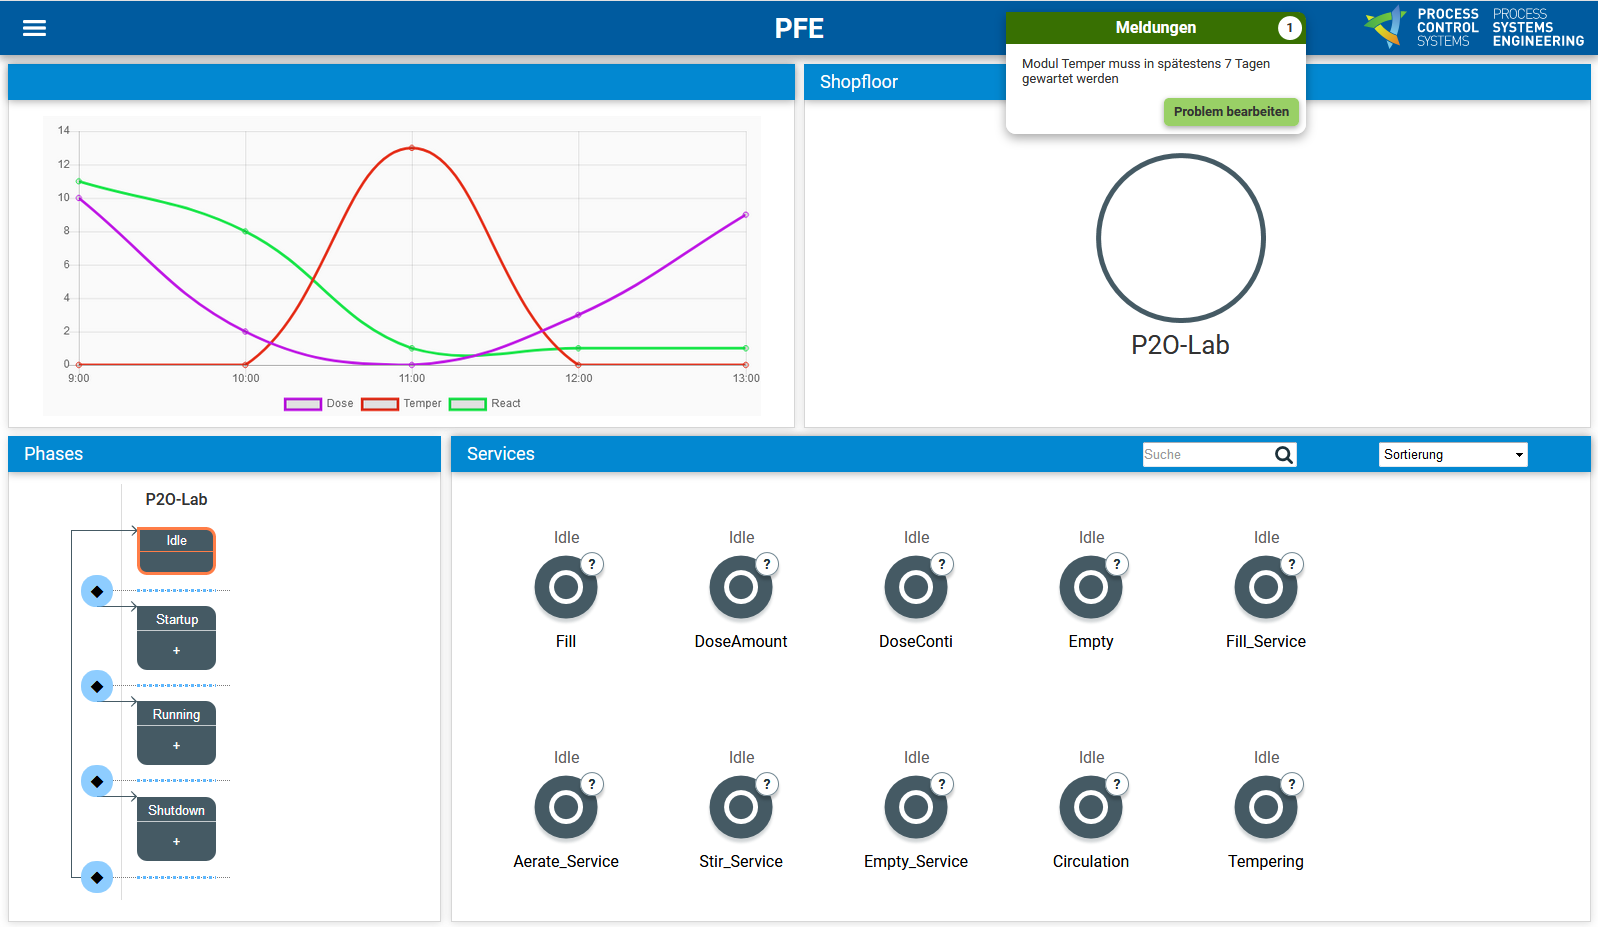
\includegraphics[angle=90, scale=0.47]{DA_files/Bilder/Konzept/Skizze-PFE.png}
\caption{Prozessführungsebene}
\label{pic:pD-PFE}
\end{figure}

\subsection{Problem beschreiben}
Das Feld für die Problembeschreibung ist in zwei Bereiche geteilt (siehe Bild \ref{pic:pD-Problembeschreibung}). Der erste Bereich umfasst die Problembeschreibung und eine (oder mehrere) Spezifikationen. Eine Spezifikation kann z.B. die Dauer der Wartung sein. Diese ist vom Modulherrsteller angegeben und kann nicht verändert werden. Der zweite Bereich stellt die Ziele dar. Über das \textbf{+} ist es möglich Ziele hinzuzufügen (siehe Bild \ref{pic:pD-Problembeschreibung-Ziel-hinzufuegen}). Das Löschen eines Ziels kann durch markieren und anschließendes klicken auf den Mülleimer durchgeführt werden (siehe Bild \ref{pic:pD-Problembeschreibung-Ziel-loeschen}). Neben diesen Fakten wird dem Nutzer auch noch visuell dargestellt, welche Bereiche vom Problem betroffen sind.
Hat der Nutzer alles erfasst und die notwendigen Ziele definiert, so kann er über den Button \textbf{Lösungen finden} das Assistenzsystem nach möglichen Lösungen fragen.

\begin{figure}[htbp]
\centering
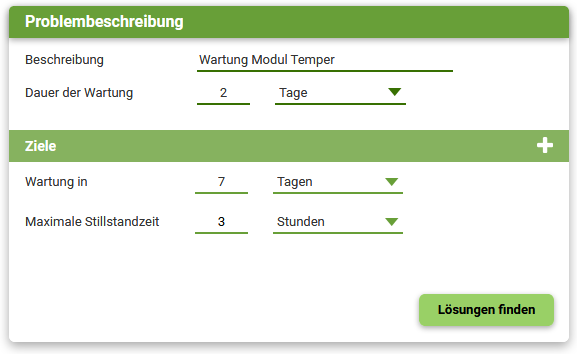
\includegraphics[scale=0.7]{DA_files/Bilder/Konzept/Skizze-Problem-1.png}
\caption{Problembeschreibung}
\label{pic:pD-Problembeschreibung}
\end{figure}

\begin{figure}[htbp]
\centering
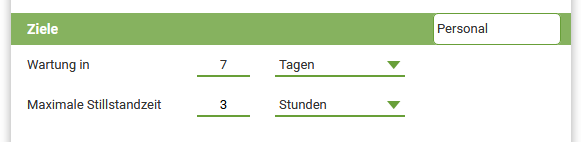
\includegraphics[scale=0.7]{DA_files/Bilder/Konzept/Skizze-Problem-Ziel.png}
\caption{Problembeschreibung - Ziel hinzufügen}
\label{pic:pD-Problembeschreibung-Ziel-hinzufuegen}
\end{figure}

\begin{figure}[htbp]
\centering
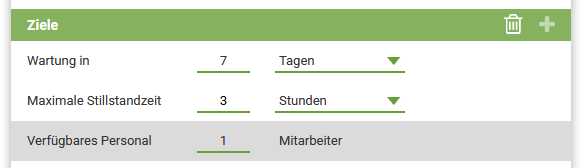
\includegraphics[scale=0.7]{DA_files/Bilder/Konzept/Skizze-Problem-loeschen.png}
\caption{Problembeschreibung - Ziel löschen}
\label{pic:pD-Problembeschreibung-Ziel-loeschen}
\end{figure}

\subsubsection*{Problem im Rezept}

\subsection{Lösungen}
\label{4:pD-Loesungen}
Die eigentliche Frage, in dem gesamten Problemlöseprozess, ist: \glqq Wie kann das Problem gelöst werden?\grqq  \ Dafür stellt das Assistenzsystem mehrere Antworten bereit. Damit der Nutzer diese gut vergleichen kann, sind die verschiedenen Lösungsmöglichkeiten in einer Tabelle dargestellt. In der ganz linken Spalte findet der Nutzer alle Informationen wieder, die bereits in der Problembeschreibung angegeben wurden. Zudem können auch noch weitere Einflussfaktoren, wie Leihkosten und Hinweise durch das Assistenzsystem ergänzt werden, um die Entscheidungsfindung des Nutzers zu erleichtern. Möchte der Nutzer nicht nur Fakten sehen, so werden durch Auswahl einer Lösung auch die Bereiche in der PFE markiert. Beim Ersetzen von einem Modul durch zwei wird sichtbar, welche Bereiche im Rezept angepasst werden müssen (siehe Abbildung \ref{pic:pD-Loesungen}). Hat der Nutzer eine Entscheidung getroffen kann er, nach Auswahl der Lösung, über den Button \textbf{Entscheiden} diese speichern und den Problemlöseprozess beenden.
\begin{figure}[htbp]
\centering
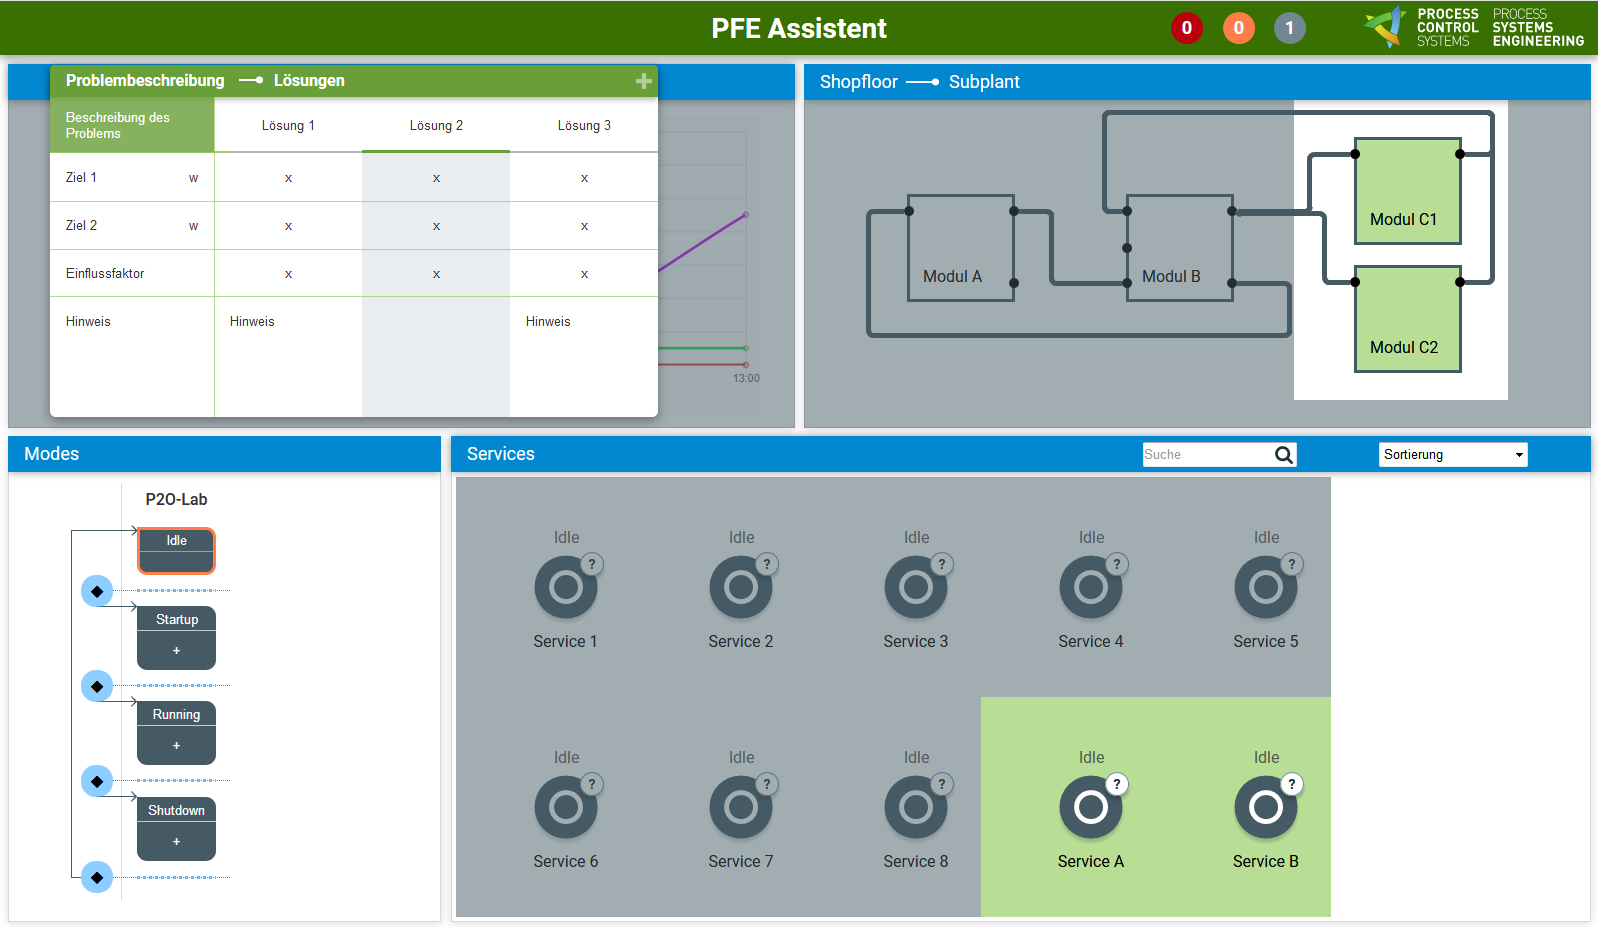
\includegraphics[angle=90,scale=0.47]{DA_files/Bilder/Konzept/Skizze-Loesungen-PFE.png}
\caption{Lösungen für das Problem}
\label{pic:pD-Loesungen}
\end{figure}

\subsection{Entscheidung}
Hat der Nutzer sich für eine Lösung entschieden, so sind keine Änderungen mehr möglich. Die Entscheidung wird hervorgehoben (siehe Bild \ref{pic:pD-Entscheidung} und analog zu den Lösungen auch in der PFE markiert. Das Assistenzsystem könnte aus dieser Entscheidung lernen und so den Wissensschatz erweitern.
\begin{figure}[htbp]
\centering
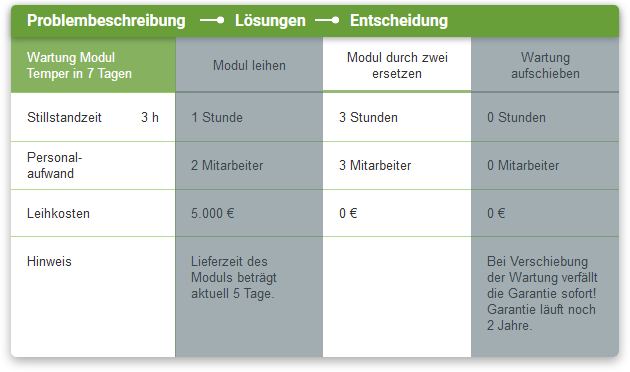
\includegraphics[scale=0.7]{DA_files/Bilder/Konzept/Skizze-Entscheidung.png}
\caption{Entscheidung für eine Lösung des Problems}
\label{pic:pD-Entscheidung}
\end{figure}

\subsection{Mehrere Probleme bearbeiten}
Über ein Seitenmenü kann der Nutzer zwischen den Problemen, die bearbeitet werden müssen, wechseln. Es wird angezeigt, ...
\begin{itemize}
\item ...wie lange noch Zeit ist, um eine Entscheidung zu treffen.
\item ...wie komplex das Problem ist. Bei einer hohen Komplexität bestehen besonders viele Zusammenhänge.
\item ...wie viele Arbeitsstunden benötigt werden, um das Problem zu lösen.
\end{itemize}
Zur Unterstützung der Lesbarkeit wurden Symbole für jede Spezifikation hinzugefügt. Eine Darstellung dessen ist in Abbildung \ref{pic:pD-Probleme-klustern} zu sehen. Dort befindet sich auch ein Symbol für Einstellungen. Dies ermöglicht, bei Weiterentwicklung des Prototypen, einen erweiterten Funktionsumfang.

\begin{figure}[htbp]
\centering
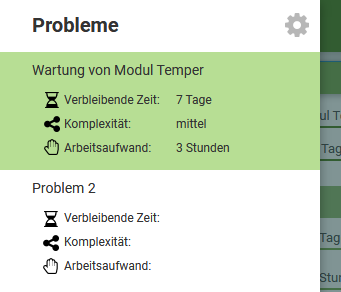
\includegraphics[scale=0.8]{DA_files/Bilder/Konzept/Skizze-Klustern-Problem.png}
\caption{Klustern von Problemen}
\label{pic:pD-Probleme-klustern}
\end{figure}
\chapter{Prototyp}
\label{Prototyp}
Im Konzept ist beschrieben, welche Funktionen umgesetzt werden müssen und wie die Informationen für den Problemlöseprozess dargestellt werden können. In diesem Abschnitt wird das Konzept ist das Design der PFE eingegliedert und prototypisch dargestellt.

Der Prototyp wird mit dem Programm Axure \todo{Verweis} umgesetzt. Dieses bietet die Möglichkeit digitale Prototypen sehr umfangreich umzusetzen.
\\ \\
Während des Problemlöseprozess nimmt das Systeme verschiedene Zustände an (siehe Abbildung \ref{pic:Zustandsdiagramm-Assistenzsystem}). Zu Beginn ist nur die grundlegende PFE dargestellt. Nach sieben Sekunden zeigt das System beispielhaft eine Meldung an. Nach Erscheinen der Meldung hat der Nutzer die Möglichkeit auf den Button \textbf{Problem bearbeiten} zu klicken. Durch diese Aktion wird das Problem genauer angezeigt. Die Interaktionsmöglichkeiten in diesem Zustand sind in Abschnitt \ref{5:Problembeschreibung}  näher beschrieben. Nach der Begutachtung und Spezifikation des Problems wechselt das Assistenzsystem durch Betätigung des Button\textbf{ Lösungen finden}, abhängig von den eingegebenen Zielen, in den Zustand der Lösungen. Soll das Problem bearbeitet werden so kann in den Zustand Problem durch klicken auf \textbf{Problembeschreibung} gewechselt werden.

\begin{figure}[tbp]
\centering
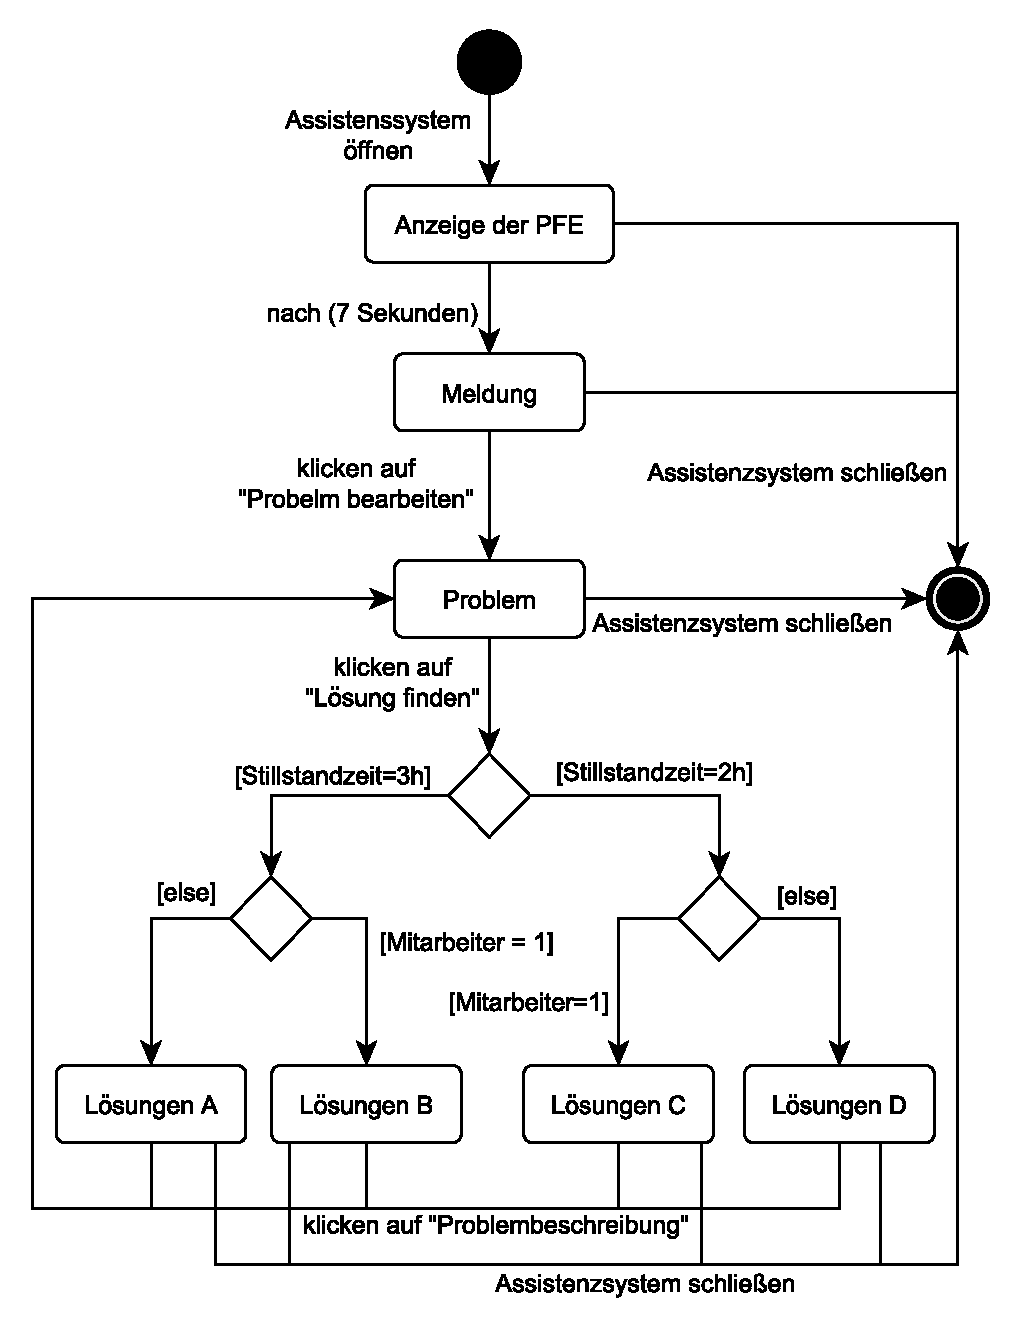
\includegraphics[scale=0.65]{DA_files/UML/Prototyp/Zustandsdiagramm-Assistenzsystem.pdf}
\caption{Zustandsdiagramm Assistenzsystem - Prototyp}
\label{pic:Zustandsdiagramm-Assistenzsystem}
\end{figure}

\section{Prozessführungsebene}
Da das Assistenzsystem in die bestehende Prozessführungsebene eingegliedert wird, müssen die grundlegenden Funktionalitäten dieser zunächst im Prototyp nachgebaut werden. Die grafischen Elemente liegen bereits in geeigneter Form vor und werden nur noch korrekt verknüpft. Dies umfasst zum einen die Elemente innerhalb der Bereiche (vgl. Abschnitt \ref{3:PFE}), als auch die Verknüpfungen zwischen den Bereichen.

\subsection{Navigation}
In der Navigation kann die Ansicht zwischen dem Shopfloor und der ausgewählten Subplant  gewechselt werden (siehe Abbildung \ref{pic:Zustandsdiagramm-Navigation}). Da die Veränderung des Zustand in der Navigation auch die Ansicht des Rezepts verändert, werden entsprechende Signale an das Rezept gesendet.
\begin{figure}[htbp]
\centering
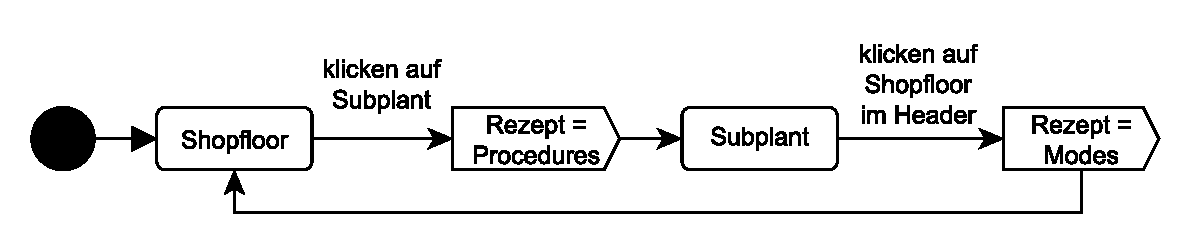
\includegraphics[scale=0.65]{DA_files/UML/Prototyp/Zustandsdiagramm-Navigation.pdf}
\caption{Zustandsdiagramm Navigation - Prototyp}
\label{pic:Zustandsdiagramm-Navigation}
\end{figure}

Zeigt die Navigation die Subplant an, kann der Nutzer durch klicken ein Modul anwählen. Diese Auswahl hat Einfluss auf die Rezeptansicht und den Service Launcher. Die entsprechenden Aktionen des Systems sind in Abbildung \ref{pic:Aktivitaetsdiagramm-Navigation-Subplant} dargestellt.
\begin{figure}[htbp]
\centering
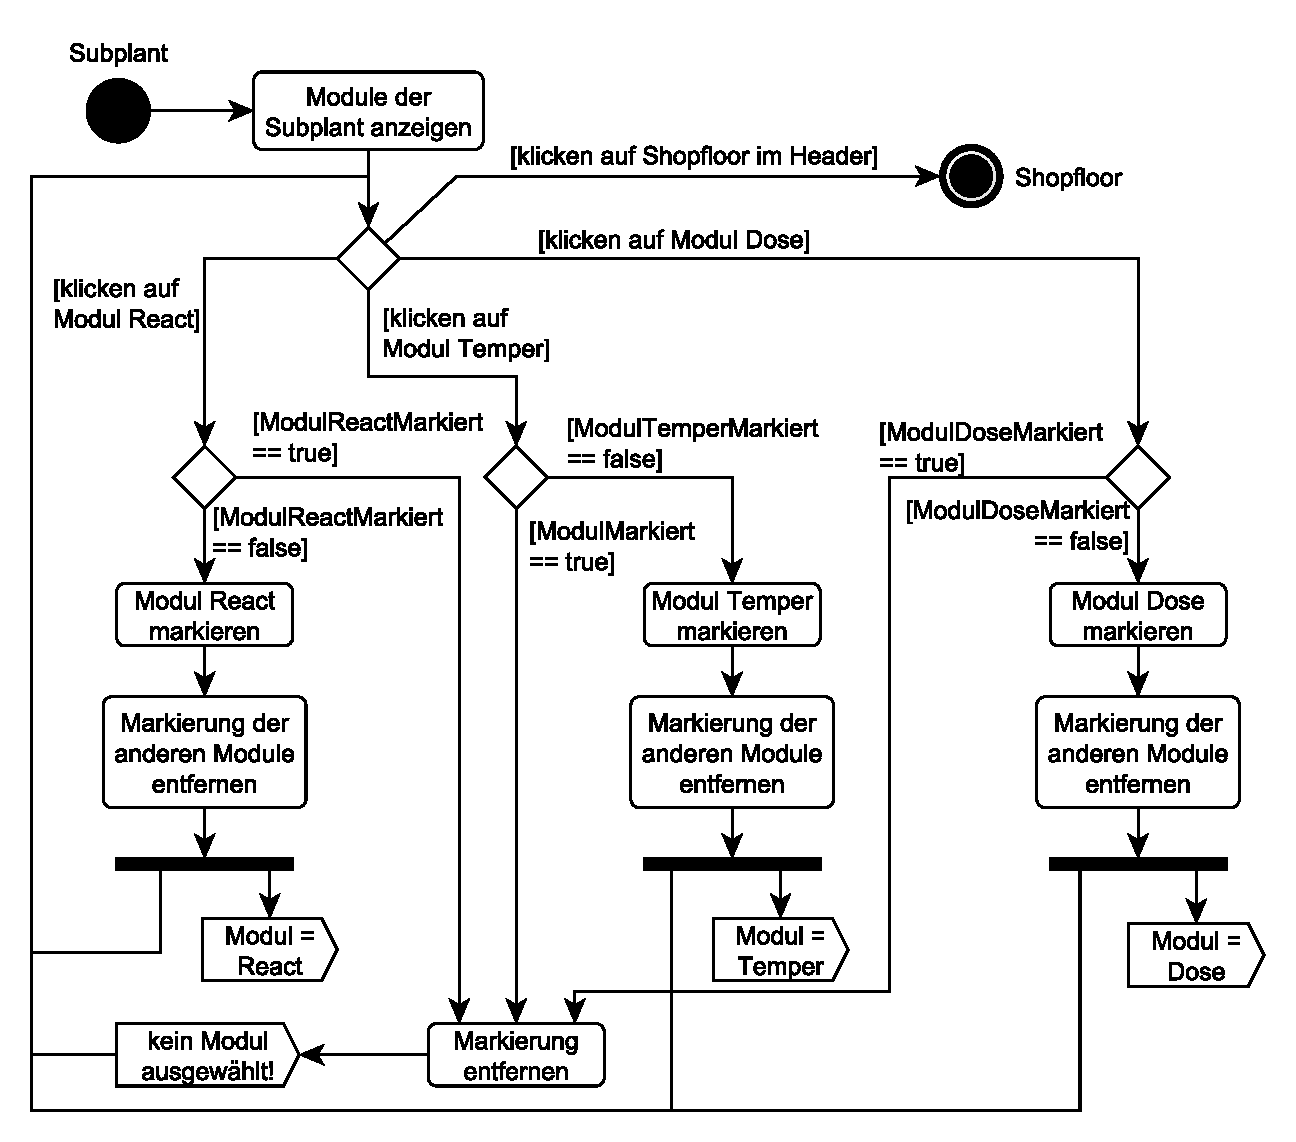
\includegraphics[scale=0.6]{DA_files/UML/Prototyp/Aktivitaetsdiagramm-Navigation-Module.pdf}
\caption{Aktivitätsdiagramm Navigation Subplant - Prototyp}
\label{pic:Aktivitaetsdiagramm-Navigation-Subplant}
\end{figure}

\subsection{Rezept}
Das Rezept zeigt entweder die Phases, die Procedures oder die Steps an. Wie zwischen diesen Ansicht gewechselt wird stellt Abbildung \ref{pic:Zustandsdiagramm-Rezept} dar.
\begin{figure}[htbp]
\centering
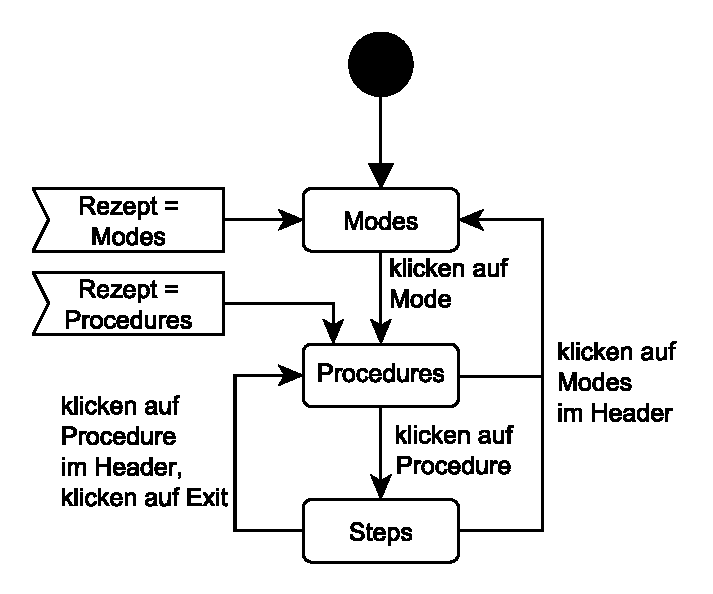
\includegraphics[scale=0.6]{DA_files/UML/Prototyp/Zustandsdiagramm-Rezept.pdf}
\caption{Zustandsdiagramm Rezept - Prototyp}
\label{pic:Zustandsdiagramm-Rezept}
\end{figure}


\todo{Procedures, Steps}
\begin{figure}[htbp]
\centering
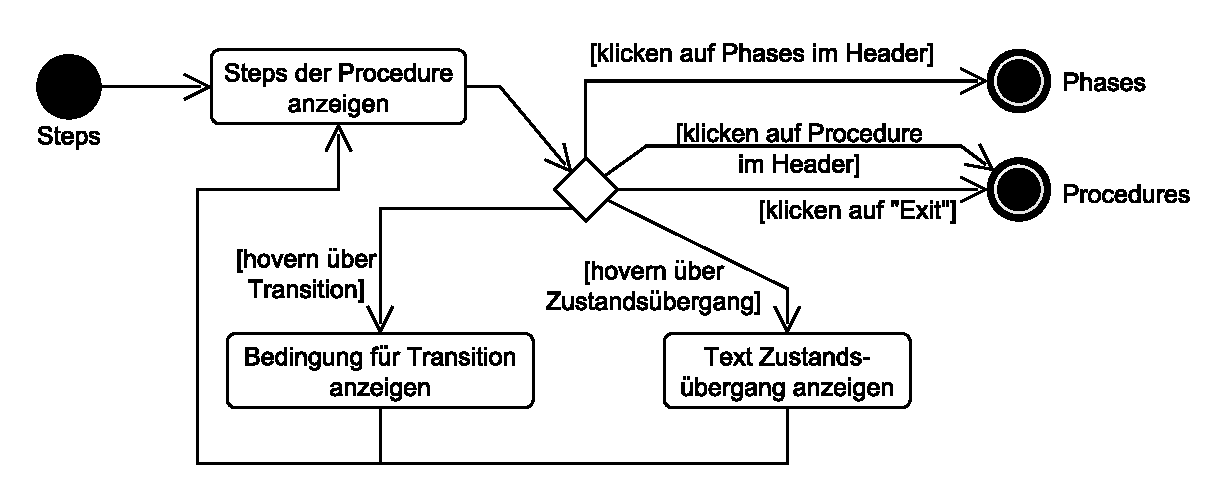
\includegraphics[scale=0.6]{DA_files/UML/Prototyp/Aktivitaetsdiagramm-Rezept-Steps.pdf}
\caption{Aktivitätsdiagramm Rezept Steps - Prototyp}
\label{pic:Aktivitaetsdiagramm-Rezept-Steps}
\end{figure}

\subsection{Service Launcher}
Der Service Launcher zeigt abhängig von der gewählten Sortierung und dem ausgewählten Modul in der Navigation die Services an. Der Nutzer hat zudem die Möglichkeit durch klicken auf den Service weitere Informationen zu bekommen. Das Verhalten des Systems wird durch Abbildung \ref{pic:Aktivitaetsdiagramm-ServiceLauncher} beschrieben.

\begin{figure}[htbp]
\centering
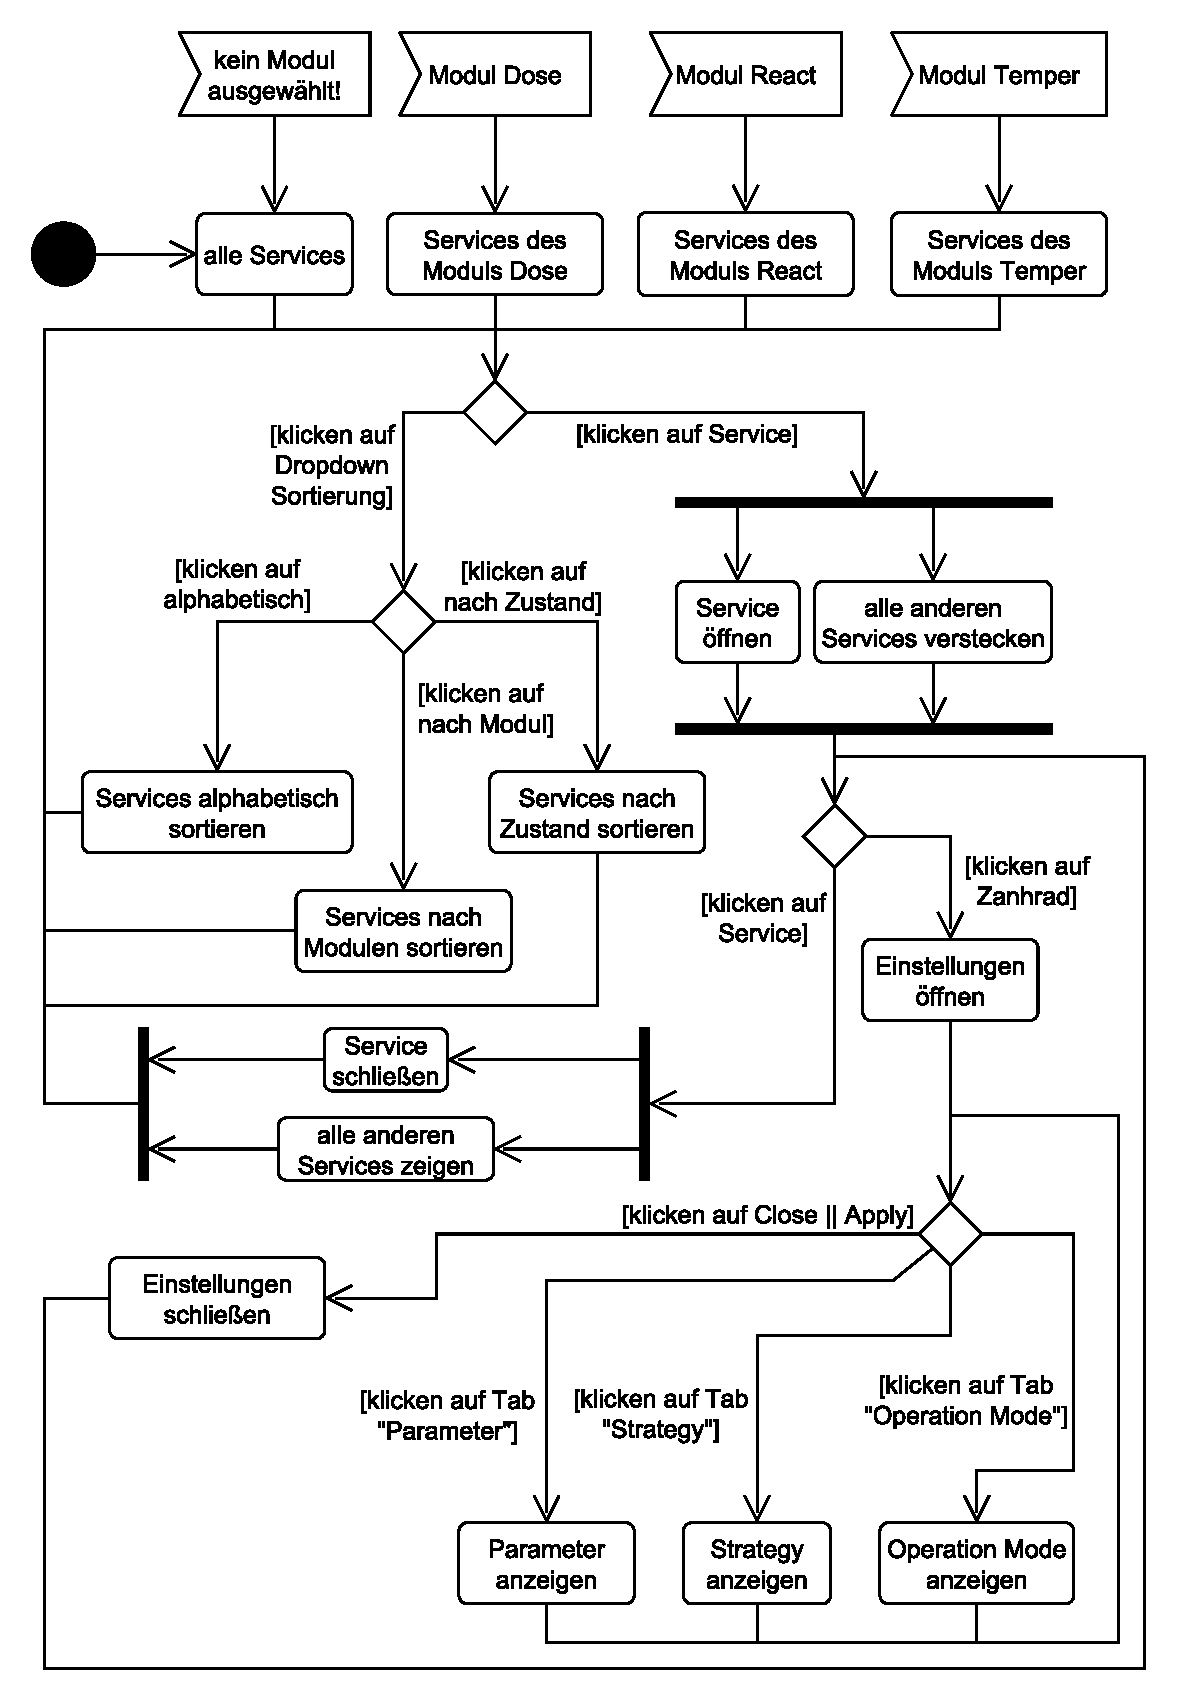
\includegraphics[scale=0.65]{DA_files/UML/Prototyp/Aktivitaetsdiagramm-ServiceLauchner.pdf}
\caption{Aktivitätsdiagramm Service Launcher - Prototyp}
\label{pic:Aktivitaetsdiagramm-ServiceLauncher}
\end{figure}

\section{Problembeschreibung}
\label{5:Problembeschreibung}
Im Konzept sind bereits die Funktionalitäten für die Problembeschreibung erläutert. Im Rahmen des Prototypen sind diese konkret umgesetzt. Der Nutzer hat die Möglichkeit ein weiteres Ziel nicht nur hinzuzufügen, sondern auch wieder zu löschen. Zudem ist das Ziel Stillstandzeit editierbar. Die Veränderung der Ziele hat einen Einfluss auf die Lösungen, welche in Abschnitt \ref{5:Loesungen} näher spezifiziert sind. Keinen Einfluss hat in diesem Beispiel die Veränderung im Dropdown-Menü. Möchte der Nutzer sich die Lösungen ansehen bringt ihn der Button Lösungen finden dort hin. Wie das Assistenzssystem auf die Interaktionen des Nutzers reagiert ist in Abbildung \ref{pic:Aktivitaetsdiagramm-Problem} dargestellt.

\begin{figure}[tbp]
\centering
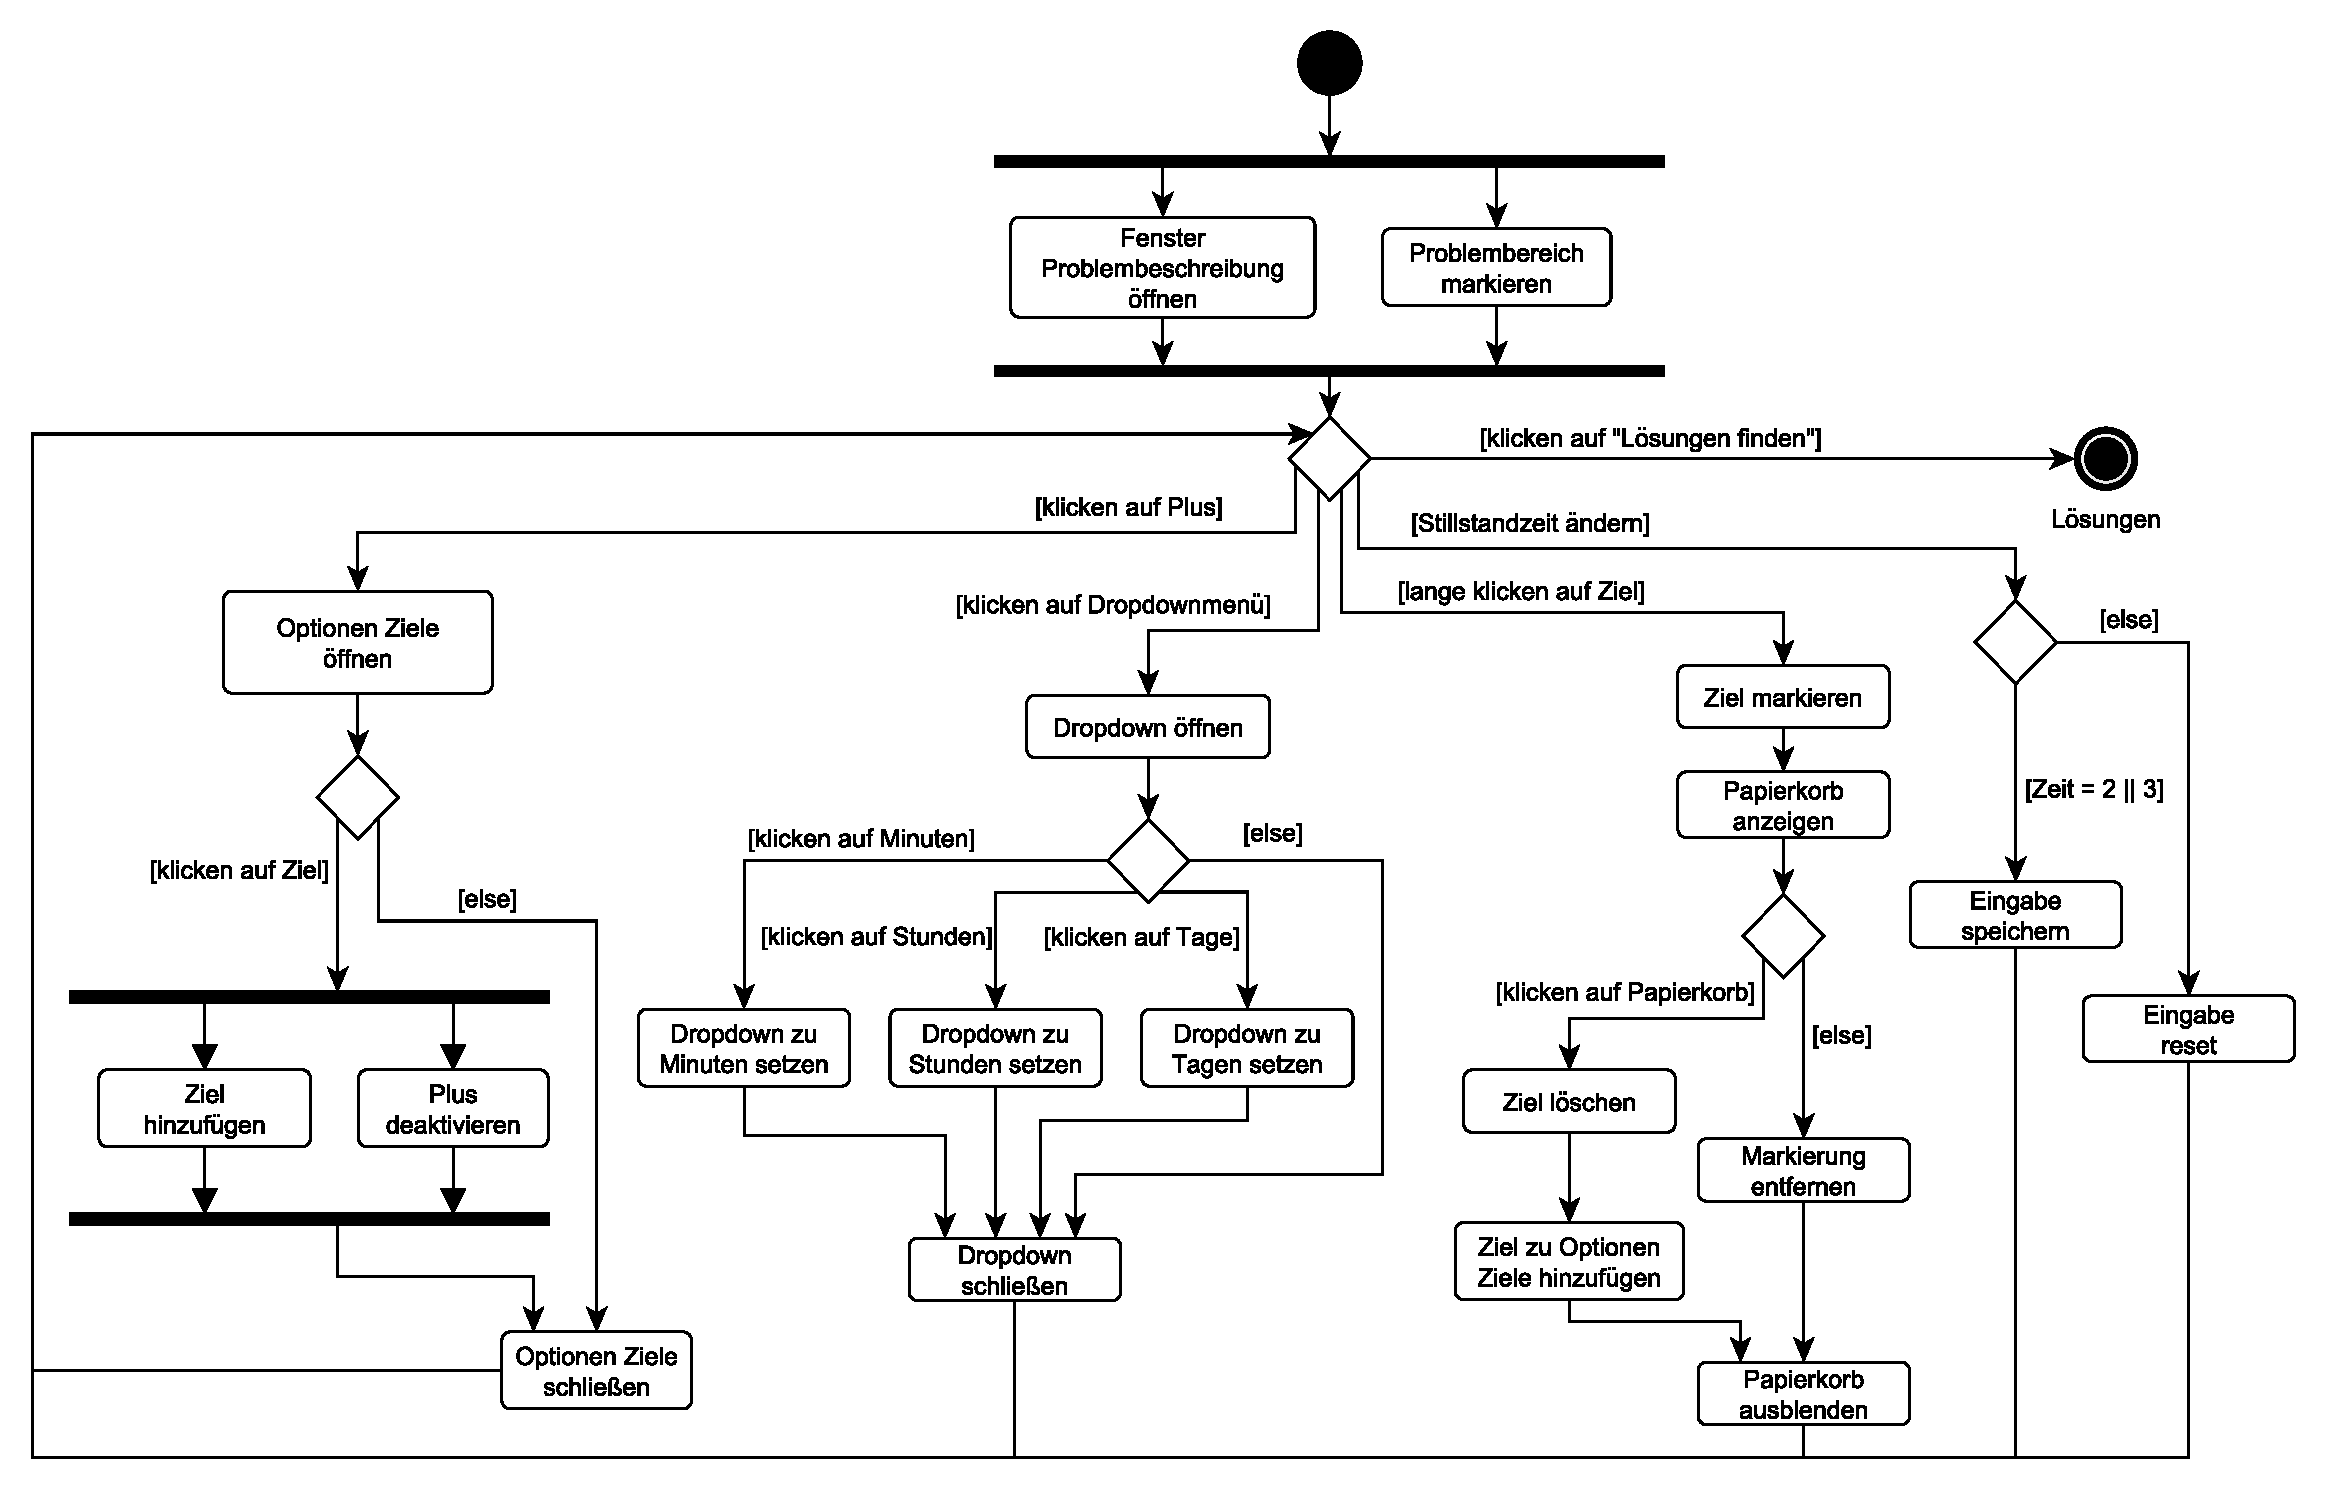
\includegraphics[angle=90,scale=0.5]{DA_files/UML/Prototyp/Aktivitaetsdiagramm-Problem.pdf}
\caption{Aktivitätsdiagramm Zustand Problem - Prototyp}
\label{pic:Aktivitaetsdiagramm-Problem}
\end{figure}

\section{Lösungen}
\label{5:Loesungen}
Die präsentierten Lösungen durch das Assistenzsystem orientieren sich an den eingegebenen Zielen des Nutzers. Der Nutzer hat die Möglichkeit durch anwählen einer Lösung sich die Veränderung in der Navigation, dem Rezept und dem Service Launcher anzusehen. Wie das Assistenzsystem auf die Auswahl des Nutzer reagiert ist in Abbildung \ref{pic:Aktivitaetsdiagramm-Loesungen} dargestellt. Die Interaktionsmöglichkeiten der Prozessführungsebene verändern sich dabei nicht.

\begin{figure}[htbp]
\centering
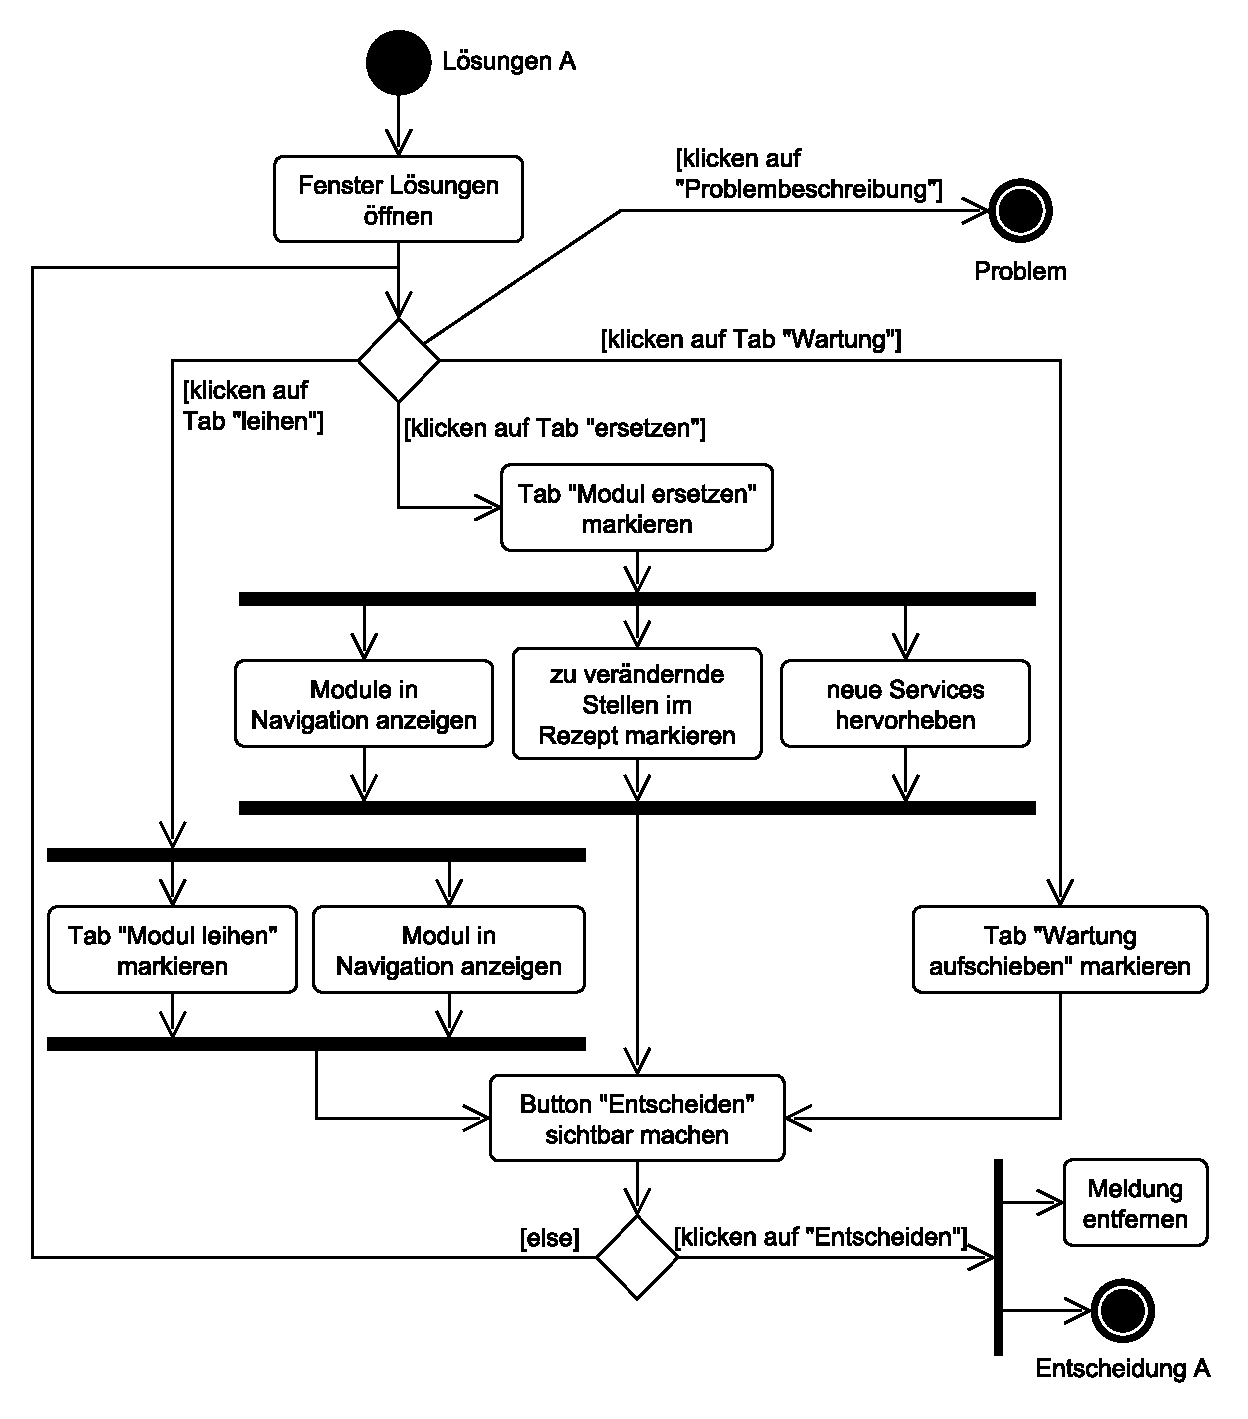
\includegraphics[scale=0.6]{DA_files/UML/Prototyp/Aktivitaetsdiagramm-Loesungen.pdf}
\caption{Aktivitätsdiagramm Lösungen - Prototyp}
\label{pic:Aktivitaetsdiagramm-Loesungen}
\end{figure}
\chapter{Validierung}
\label{Validierung}

Ziel der Diplomarbeit ist die Entwicklung einer nutzerfreundliche Oberfläche zur Problemlösung in modularen Anlangen. Dieses Kapitel beantwortet, wie gut die Umsetzung geglückt ist. Dazu werden zunächst die Anforderungen an das Assistenzsystem ausgewertet. 

\section{Vergleich mit Anforderungen}
In Abschnitt \ref{3:Anforderungen} wurden Anforderungen an das Assistenzsystem gestellt. Die Erfüllung der Anforderungen wird im Folgenden diskutiert. Eine erste Einschätzung gibt jeweils eine Tabelle. Ein + bedeutet voll erfüllt, ein o bedeutet teilweise erfüllt und ein - bedeutet nicht erfüllt.

\subsection{Unterstützung der Problemidentifikation}
Der Nutzer soll bei der Problemidentifikation unterstützt werden. Tabelle \ref{tab:Anforderungen-Problemidentifikation} stellt dar, wie gut die einzelnen Anforderungen durch den Prototypen erfüllt sind.
\begin{table}[htbp]
\caption{Auswertung Anforderungen Problemidentifikation}
\centering
\begin{tabular}{l|c|c|c|c|c|c}
\textbf{Anforderung} & PI 1.1 & PI 1.2 & PI 1.3 & PI 2 & PI 3 & PI 4 \\
\hline
\textbf{Erfüllt} & o & + & o & + & + & + \\
\end{tabular}
\label{tab:Anforderungen-Problemidentifikation}
\end{table}

Insgesamt ist die Unterstützung der Problemidentifikation als positiv zu werten. Es gibt lediglich noch Anpassungsbedarf bei der Problembeschreibung. Dem Nutzer wird aktuell nicht die Möglichkeit gegeben selber ein Problem zu melden. Weitere Details und Begründungen zu der Bewertung sind im Folgenden erläutert.

\subsubsection*{PI 1.1 Problembeschreibung}
Dem Nutzer sollte die Möglichkeit gegeben werden das Problem zu beschreiben. Der Prototyp erfüllt diese, indem sowohl textuell die Beschreibung verändert werden kann, als auch die Parameter der Rahmenbedingung verändert werden können. Ein Beispiel dafür ist die Wartungsdauer. Der Nutzer kann in Absprache mit dem Hersteller festlegen, wie lange die Wartung für das Modul dauert.

Hat der Nutzer selber ein Problem entdeckt, ist es derzeit nicht möglich dieses zu beschreiben. Dafür müsste zunächst näher untersucht werden, welche Probleme die modulare Anlage nicht selber erkennt und durch den Nutzer ausgelöst werden müssen. Das könnten beispielsweise Flüssigkeiten sein, die auslaufen oder komische Geräusche. Erste Ideen gab es dazu bereits in xx \todo{Oberseminar}. Es ist zu prüfen, ob diese Ansätze auch für die modularen Anlagen umgesetzt werden können. Des Weiteren wäre interessant, ob das Assistenzsystem die Informationen auch hilfreich verarbeiten kann. Wenn der Nutzer diesem mitteilt, wo Flüssigkeit ausläuft, weiß das Assistenzsystem dann, welcher Service damit zusammen hängt?

\subsubsection*{PI 1.2 Zieldefinition}
Dem Nutzer sollte die Möglichkeit gegeben die Ziele zu definieren, um anhand diese die Lösungen zu finden. Der Prototyp erfüllt diese, indem sich die Parameter der Ziele verändern lassen.

\subsubsection*{PI 1.3 Informationen}
In den Anforderungen steht, dass dem Nutzer alle relevanten Informationen über die aktuelle Situation zur Verfügung stehen sollen. Die Auswertung dieser Anforderung gestaltet sich sehr schwierig, da die Anforderung sehr unspezifisch formuliert ist.

Abgeleitet aus der Analyse ist mit allen relevanten Informationen Folgendes gemeint:
\begin{itemize}
\item Aktueller Zustand der Anlage: KPIs, Rezept, Services
\item Informationen über den Produktionsprozess, z.B.:
	\begin{itemize}
	\item Wie sehr ist die aktuelle Anlage ausgelastet?
	\item Wie gut ist die Qualität meiner Produktion?
\end{itemize}
\end{itemize}
Davon ausgehend ist die Frage zu beantworten, ob die KPIs die Informationen über den Produktionsprozess abdecken. Wenn sie dies nicht tun, muss untersucht werden, wie die Informationen über den Produktionsprozess sinnvoll eingebunden werden können. Zu berücksichtigen ist unter anderem, dass es sowohl modulspezifische, als auch anlagenspezifische Informationen geben kann. Des Weiteren stellt sich noch die Frage, ob die KPIs im MTP vordefiniert werden können und wie der Anlagenbetreiber selber welche erstellen kann.

Die aktuelle Situation umfasst im Rahmen dieser Arbeit nur die modulare Anlage. Ein Produktionsprozess kann aber noch durch weitere Faktoren beeinflusst werden. Relevant sind auch die Umgebungsbedingungen, wie die Umgebungstemperatur, und die Mitarbeiter, die an der Anlage arbeiten. Welchen Einfluss diese auf den Problemlöseprozess haben wurde in dieser Arbeit nicht untersucht.

Um die Anforderung allumfassend zu bewerten, müsste genau festgelegt werden, welche KPIs angezeigt werden sollen und welche Informationen über den Produktionsprozess relevant sind. Beides ist jedoch stark abhängig von den Bedürfnissen des Betreibers der modularen Anlagen. Die vorhandene PFE wurde dazu entwickelt den Produktionsprozess zu überwachen und erfüllt damit die Anforderung.

\subsubsection*{PI 2 Unterstützung bei Problemidentifikation}
Das Assistenzsystem unterstützt den Nutzer bei der Problemidentifikation mit Meldungen, Warnungen und Alarme. Dadurch wird der Nutzer auf Probleme aufmerksam gemacht.

\subsubsection*{PI 3 Ziele hinzufügen}
Der Nutzer hat im Feld der Problembeschreibung die Möglichkeit für ihn relevante Ziele hinzuzufügen und irrelevante Ziele zu löschen.

\subsubsection*{PI 4 Problembereich}
Dem Nutzer wird der Auslöser des Problems durch die Problembeschreibung mitgeteilt. Der Problembereich wird hervorgehoben, indem irrelevante Informationen durch graue halbdurchsichtige Felder verdeckt werden.

\subsection{Unterstützung bei der Problemlösung}
Wie der Titel der Arbeit schon sagt liegt der Schwerpunkt auf der Problem\textbf{lösung}. Tabelle \ref{tab:Anforderungen-Problemlösung} zeigt leider nur eine teilweise Erfüllung der Anforderungen. Hintergrund ist einerseits die fehlende Möglichkeiten im Protoyp eigene Lösungen hinzuzufügen. Andererseits sieht der Nutzer nicht, wie sich seine Entscheidung auf die Produktqualität oder die Unternehmensziele auswirkt.
\begin{table}[htbp]
\caption{Auswertung Anforderungen Problemlösung}
\centering
\begin{tabular}{l|c|c|c|c|c}
\textbf{Anforderung} & PL 1 & PL 2 & PL 3.1 & PL 3.2 & PL 4 \\
\hline
\textbf{Erfüllt} & + & o & o & o & - \\
\end{tabular}
\label{tab:Anforderungen-Problemlösung}
\end{table}

\subsubsection*{PL 1 Assistenz schlägt Lösungen vor}
Das Assistenzsystem wertet die definierten Ziele des Nutzer aus, sucht nach geeigneten Lösungen und präsentiert diese dem Nutzer. Im Falle des Prototypen sind die Lösungen vordefiniert. Für zukünftige Arbeiten wäre es interessant zu erfahren, welche Möglichkeiten im Rahmen der modularen Anlage existieren. Wichtig dabei zu berücksichtigen ist der Unterschied zwischen modulspezifischen und anlagenspezifischen Problemen. Modulspezifisch bedeutet, dass sich das Problem auf das konkrete Modul bezieht und es irrelevant ist mit welchen anderen Modulen eine Verbindung besteht. Anlagenspezifische Probleme sind nur im Kontext aller verbundenen Module zu betrachten. Wenn die Module also anders verbunden werden ändern sich auch die Zusammenhänge von Problem und Lösungen.

\subsubsection*{PL 2 Nutzer schlägt Lösungen vor}
Dem Nutzer sollte es möglich sein selber Lösungen vor zu schlagen. Durch das Plus-Symbol im Reiter Lösungen ist das zwar angedacht, aber nicht ausgeführt. Um sich Gedanken zu machen, wie Lösungen eingegeben werden können, muss im ersten Schritt geklärt werden, was der Nutzer eingeben möchte. Im Rahmen des Modultausch ist es denkbar noch mehr andere Module in Erwägung zu ziehen. Dazu könnte der PEA-Manager von Jan Funke \cite{Funke2018} eingebunden werden. So kann der Nutzer geeignete Module auswählen. Ungeklärt bleibt die Frage, wie kreative Lösungen eingebunden werden können. Beispielhaft könnte man vorübergehend eine andere Anlage still legen und ein Modul aus dieser nutzen.

\subsubsection*{PL 3.1 Auswirkung auf Anlage / Prozess}
Der Prototyp zeigt dem Nutzer an, welche Veränderungen sich in der modularen Anlage durch die Lösung ergeben. Es werden Veränderungen im Rezept, in der Navigation und in den Services angezeigt. Die verfahrenstechnischen Auswirkungen auf den Prozess sind nicht dargestellt. Es ist also nicht abschätzbar, wie sich die Produktqualität durch die Lösung verändern könnte. Denkbar sind dazu Anbindungen an eine virtuelle modulare Anlage, die mögliche Veränderungen berechnet und dem Nutzer mitteilt.

\subsubsection*{PL 3.2 Einflussfaktoren}
Dem Nutzer wird durch das Assistenzsystem angezeigt, welche Einflussfaktoren sich zahlenmäßig unterscheiden. Im Konzept ist vorgesehen, dass alle relevanten Einflussfaktoren sichtbar sind (vgl. \ref{3:Anforderungen}). Relevant bedeutet, dass die Einflussfaktoren zuvor von dem Unternehmen oder dem Mitarbeiter als wichtig definiert wurden.

Die Tatsache, dass auch die Abhängigkeiten der Services einen Einfluss haben ist zwar angedacht aber nicht umgesetzt. Grund dafür ist eine noch fehlende Grundlage im MTP. In diesem Zusammenhang ist auch interessant, wie sich die Abhängigkeiten darstellen lassen. Denkbar ist eine hierarchische Gliederung \todo{Ideen spinnen}

\subsubsection*{PL 4 Lösungen bewerten}
Angedacht in der Anforderung ist es, dass der Nutzer die einzelnen Lösungen bewerten kann, um eine Entscheidung zu treffen. Diese Anforderung wurde nicht umgesetzt, da eine Lösung nicht richtig oder falsch sein kann. Es ist möglich, dass eine Lösung besser oder schlechter ist, als eine andere. Die Bewertung dieser ist aber stark von der Gesamtsituation (z.B. verfügbare Mitarbeiter, Auftragslage) und dem Wissen des Mitarbeiters abhängig. Diese Anforderung ist daher kritisch zu hinterfragen. In welchem Rahmen macht eine Bewertung der Lösungen Sinn? Wird die Bewertung von dem Assistenzsystem verarbeitet? Wenn die Bewertung verarbeitet wird, wie wirkt sie sich auf zukünftige Problemlösungen aus? Diese und weitere Fragen sind noch zu beantworten.

\subsection{Klustern von Problemen}
Probleme sollen geklustert werden, damit mehrere Probleme parallel bearbeitet werden können. Wie Tabelle \ref{tab:Anforderungen-Probleme} zeigt, sind die Anforderungen größtenteils erfüllt. 

Grund dafür ist, dass zur Zeit nur das Assistenzsystem die Probleme mit Merkmalen versieht und klustert. \todo{Im Konzept anders vorsehen?}

\begin{table}[htbp]
\caption{Auswertung Anforderungen: Probleme klustern}
\centering
\begin{tabular}{l|c|c|c}
\textbf{Anforderung} & KP 1 & KP 2 & KP 3\\
\hline
\textbf{Erfüllt} & + & o & + \\
\end{tabular}
\label{tab:Anforderungen-Probleme}
\end{table}

\subsubsection*{KP 1 Mehrere Probleme bearbeiten}
Laut Anforderung sollte der Nutzer die Möglichkeit haben mehrere Probleme gleichzeitig bearbeiten zu können. Das ist vor allem dann relevant, wenn eine Entscheidung nicht sofort getroffen werden muss. Der Nutzer kann das Problem später weiter bearbeiten und sich in der Zwischenzeit einem anderen zuwenden. Die Interaktionsplattform macht das durch die linke Seitenleiste möglich, in der das zu bearbeitende Problem ausgewählt werden kann. Ebenso ist denkbar, dass eine Problembearbeitung durch ein neues, akuteres, Problem unterbrochen wird.

\subsubsection*{KP 2 Probleme sortieren}
Da im Prototyp nur ein Problem realisiert ist erfolgt keine konkrete Sortierung der Probleme. Das Konzept sieht jedoch eine Sortierung anhand von Zeit, Komplexität und Arbeitsaufwand vor, wodurch die Anforderung erfüllt ist. Offen bleibt die Frage, ob diese Sortierung für den Mitarbeiter ausreichend ist oder dort noch weitere Wünsche bestehen.

\subsubsection*{KP 3 Merkmale der Probleme}
Derzeit versieht das Assistenzsystem die Probleme mit den in den Anforderungen definierten Merkmalen. Es wurde jedoch zu Beginn dieser Arbeit keine Umfrage durchgeführt, welche Merkmale der Nutzer sich wünscht. Dadurch bleibt offen, ob der Nutzer noch weitere Merkmale hinzufügen möchte oder andere Merkmale wünscht.

\section{Aspekte des Assistenzsystems}
Neben den individuell definierten Anforderungen an das Assistenzsystem, gibt es eine Reihe an Anforderungen, die durch die Literatur gegeben sind. \todo{Einleitung schreiben}

\subsection*{Eingliederung in Automatisierungsgrad}
Abschnitt \ref{3:Anpassung-Aufgabe} macht deutlich, dass sich das Assistenzsystem anhand des Zeitdrucks anpassen sollte. Im Prototypen ist das Problem nicht zeitkritisch und sieht daher einen geringen Automatisierungsgrad vor. In die 10 Level der Automatisierung von Sherdian \cite{Wandke2005} lässt sich der Prototyp auf Level 3 einordnen. Bei einem höheren Zeitruck sind auch die Stufen 4 und 5 in Betracht zu ziehen. Level 6 ist im Sinne der kollaborativen Assistenz nicht anzuwenden, da auf diesem Level die Möglichkeiten des Nutzers stark eingeschränkt sind. Es ist noch zu untersuchen, in welchen Problemfällen welcher Autonomiegrad angewendet wird. Dazu sollten auch die Autonomiestufen in der Prozessindustrie von Schegner \cite{Schegner2017} betrachtet werden. In dieses System lässt sich der Prototyp auf Stufe 1 einordnen.

\subsection*{Aufgaben von digitaler Assistenz}
Digitale Assistenz kann eine ganze Reihe an Aufgaben übernehmen (vgl. Abschnitt \ref{2:Einsatz-Assistenz}). Tabelle \ref{tab:Aufgaben-Assistenz-Prototyp} stellt dar, welche Aufgaben im Rahmen des Konzepts übernommen werden und wie sich dies im Prototyp äußert.

\begin{table}
\caption{Aufgaben digitaler Assistenz, die durch den Prototypen erfüllt werden}
\centering
\begin{tabular}{l|c|p{0.54 \textwidth}}
\textbf{Aufgabe} & \textbf{Übernahme} & \textbf{Erläuterung} \\
\hline
Warnung & o & Der Nutzer wird nur durch die Hinweise in den Lösungen vor Fehlentscheidungen gewarnt.\\
\hline
Signale & + & Es wird dem Nutzer angezeigt, welche Änderungen sich ergeben.\\
\hline
Orientierung & + & Der Nutzer kann Ziele hinzufügen und entfernen \\
\hline
Kennzeichnung & o & Die Symbole werden mittels Hover-Funktionen erklärt.\\
\hline
Erklärung & - & Die Auswahl der Lösungen wird nicht erklärt.\\
\hline
Bereitstellung & o & Das Assistenzsystem stellt nur eine ausgewählte Menge und nicht alle an Informationen zur Verfügung.\\
\hline
Filter & + & Das Assistenzsystem zeigt nur relevante Daten zur Entscheidungsfindung an.\\
\hline
Berater & o & Das Assistenzsystem liefert mehrere Vorschläge, macht aber keinen Vorschlage, welche Option die Beste sein könnte. \\
\hline
Delegieren & - & Das Assistenzsystem unterstützt den Nutzer aktuell nicht bei der Anwendung der ausgewählten Lösung.\\
\end{tabular}
\label{tab:Aufgaben-Assistenz-Prototyp}
\end{table}

\subsection*{Ergonomisch gute Gestaltung}
Anforderungen an eine ergonomische gute Gestaltung gibt es viele. Die Erläuterung zu den Grundsätzen der Dialoggestaltung und den Aspekten für gute Informationsdarstellung finden sich in Abschnitt \ref{2:ergonomische-Gestaltung}. In Tabelle \ref{tab:Validierung-Dialoggestaltung} wird deutlich, dass im Durchschnitt die Grundsätze der Dialoggestaltung eingehalten wurden. Lediglich die Individualisierbarkeit wurde nicht erfüllt, weil der Nutzer das System nicht selber anpassen kann. Jedoch ist diese Anforderung überholt, wenn sich das System an den Nutzer anpasst. Eine umfangreiche Auswertung zur Individualisierung findet sich im nächsten Abschnitt.

\begin{table}
\caption{Validierung: Grundsätze der Dialoggestaltung}
\centering
\begin{tabular}{p{0.2 \textwidth}|c|p{0.55 \textwidth}}
\textbf{Grundsatz} & \textbf{Erfüllt} & \textbf{Erläuterung} \\
\hline
Aufgaben-angemessenheit & + & Der Use Case konnte mit dem Prototypen erfolgreich umgesetzt werden. \\
\hline
Selbst-beschreibungs-fähigkeit & + & Durch die Anzeige oben in der Leiste weiß der Nutzer jederzeit an welcher Position er sich befindet. \\
\hline
Erwartungs-konformität & + & Die Gestaltung des Assistenzsystem orientiert sich an der PFE.\\
\hline
Lern-förderlichkeit & o & Es gibt keine konkrete Unterstützung im Sinne von Erläuterungen. Durch eine eindeutige Beschreibung der Buttons ist der Prototyp jedoch leicht zu verstehen. \\
\hline
Steuerbarkeit & + & Durch das Setzen der Ziele kann der Nutzer die Richtung steuern. Die Geschwindigkeit wird durch Betätigen der Buttons gesteuert. \\
\hline
Fehlertoleranz & + & Ziele können im Nachhinein noch mal geändert werden. \\
\hline
Individualisier-barkeit & - & Dem Nutzer stehen aktuell keine Möglichkeiten zur Individualisierung zur Verfügung. \\
\end{tabular}
\label{tab:Validierung-Dialoggestaltung}
\end{table}

Eine Auswertung der Aspekte für gute Informationsdarstellung findet sich in Tabelle \ref{tab:Validierung-Informationsdarstellung}. Bei den Aspekten \textit{Entdeckbarkeit}, \textit{Unterscheidbarkeit} und eindeutige \textit{Interpretierbarkeit} ist eine objektive Betrachtung nur schwer möglich, da dies jeder Mensch anders empfindet. Aus diesem Grund wird eine Befragung von Experten durchgeführt (siehe Abschnitt \ref{6:Nutzerbefragung}).

\begin{table}
\caption{Validierung: Aspekte für die Informationsdarstellung}
\centering
\begin{tabular}{p{0.2 \textwidth}|c|p{0.55 \textwidth}}
\textbf{Aspekt} & \textbf{Erfüllt} & \textbf{Erläuterung} \\
\hline
Entdeckbarkeit & + & Die zugrundeliegende PFE bietet die Grundlage für eine gute Wahrnehmung der Informationen. Das Assistenzsystem nutzt und erweitert dies. \\
\hline
Ablenkungs-freiheit & + & Wird durch das Verdecken der irrelevanten Informationen gewährleistet. \\
\hline
Unterscheid-barkeit & + & Durch die Tabelle sind die Informationen eindeutig zugeordnet. Die Lösungen zeigen an, welche Veränderung was beeinflusst. \\
\hline
Eindeutige Interpretierbarkeit & o & Ob die Informationen für den Nutzer eindeutig sind, kann nur durch eine Umfrage ermittelt werden.\\
\hline
Kompaktheit & + & Dem Nutzer werden nur die für die Problemlösung relevanten Informationen angezeigt. \\
\hline
Konsistenz & + & Da sich die Gestaltung am Material Design orientiert ist die Konsistenz gegeben. \\
\end{tabular}
\label{tab:Validierung-Informationsdarstellung}
\end{table}


\subsection*{Individualisierbarkeit}
Wann Individualisierung eingesetzt werden sollte beschreibt Abschnitt \ref{2:Individualisierung}. Das Konzept zum Assistenzsystem sieht vor allem Individualisierung im Sinne der \textbf{Schwankung der Aufgabenmerkmale} vor. Die \textbf{Variation der Benutzermerkmale} wird zwar in der Analyse als relevant dargestellt, jedoch im Konzept nicht weiter berücksichtigt. Im Rahmen dieser Arbeit wurde davon ausgegangen, dass sich die Benutzermerkmale nicht groß unterscheiden, da die Mitarbeiter im Umfeld der modularen Anlagen sehr ähnliche Voraussetzungen erfüllen müssen. Natürlich ist jeder Mitarbeiter individuell und hat verschiedene Fähigkeiten. Wie stark sich diese im Kontext der modularen Anlagen unterscheiden ist noch zu prüfen.

Im Sinne von Herczeg \cite{Herczeg2006} findet die Individualisierung im Prototypen auf der Intentionalen Ebene und Pragmatischen Ebene statt (vgl. Abschnitt \ref{2:Individualisierung}). Das Assistenzsystem passt sich vor allem an die Veränderungen des Problems und die definierten Ziele an. Veränderungen im Sinne verschiedener Ein- und Ausgabegeräte und Einstellungen des Nutzers werden nicht durchgeführt.

\section{Nutzerbefragung}
\label{6:Nutzerbefragung}
Für eine gute Einschätzung der Nutzerfreundlichkeit ist es notwendig, den Nutzer des Systems zu befragen. Es bringt nichts, wenn die Fakten auf dem Papier stimmen, der Benutzer aber trotzdem total unzufrieden ist. Aus diesem Grund werden im nächsten Abschnitt Möglichkeiten zur Nutzerbefragung aufgezeigt. Anschließend wird ein Test erstellt und mit einigen ausgewählten Nutzer durchgeführt. Anhand des Ergebnis kann abgeschätzt werden, welche Elemente beibehalten werden sollen und wo Verbesserungspotential vorhanden ist.

\subsection{Testmöglichkeiten}
Möchte man die Benutzerfreundlichkeit eines Systems testen, kann man den Nutzer bei Verwendung des Systems beobachten oder xxx. Laut xx ist \glqq der vielleicht offensichtlichste Weg etwas über die Nutzerfreundlichkeit von etwas zu erfahren, den Nutzer zu fragen, ob er etwas über seine Erfahrung erzählt\grqq(Measuring the User Experience S. 123) \todo{Zitat}. Dazu können verschiedene Fragen mit verschiedenen Skalen oder offene Fragen gestellt werden. Offene Fragen sind schwieriger zu analysieren, als Tests mit Skalen. Letztere lassen sich in individuelle und generalisierte Fragebögen einteilen. Individuelle Fragebögen lassen systemspezifische Fragen zu und können z.B. für die Auswahl der Testpersonen angewendet werden. Die generalisierten Fragebögen sind standardisiert und können somit auch Unterschiede zwischen verschiedenen Systemen aufzeigen. Einige dieser Fragebögen sind im Folgenden vorgestellt.

\subsubsection*{System Usability Scale}
Der SUS (System Usability Scale) Fragebogen ist ein standardisierter Fragebogen zur Bewertung der Nutzerfreundlichkeit eines Systems. Er besteht aus zehn Fragen und fünf Stufen zwischen Stimme Gar nicht zu und Stimme voll zu. Die eine Hälfte der Fragen (ungerade Zahlen) ist positiv formuliert, die andere Hälfte (gerade Zahlen) ist negativ formuliert. Für jede Frage werden abhängig von der Antwort zwischen 0 und 4 Punkte verteilt und summiert. Anschließend wird die Summe mit 2,5 multipliziert. Die Summe befindet sich auf einer Skala von 0 bis 100. Bei 100 ist die Nutzerfreundlichkeit voll erfüllt. \todo{Quelle}

\subsubsection*{User Experience Questionnaire}
Mit dem UEQ (User Experience Questionnaire) soll möglichst schnell und unmittelbare der Gesamteindruck des Nutzers eines Systems erfasst werden. Der Fragebogen besteht aus 26 Fragen und einer 7-stufigen Skala mit semantischen Differentialen, wie kompliziert und einfach. Eingeteilt sind die Fragen in folgende sechs Skalen \cite{} \todo{Zitat}:
\begin{itemize}
\item \textbf{Attraktivität:} Mag der Nutzer das System? (6 Fragen)
\item \textbf{Benutzerqualität} (jeweils 4 Fragen)
	\begin{itemize}
	\item \textbf{Vorhersagbarkeit:} Hat der Nutzer das Gefühl, das System unter Kontrolle zu haben?
	\item \textbf{Durchschaubarkeit:} Kann der Nutzer schnell erlernen, wie das System zu nutzen ist?
	\item \textbf{Effektivität:} Kann der Nutzer seine Aufgabe ohne unnötigen Aufwand bewältigen?
	\end{itemize}
\item \textbf{Designqualität} (jeweils 4 Fragen)
	\begin{itemize}
	\item \textbf{Stimulation:} Macht die Benutzung des Systems Spaß?
	\item \textbf{Originalität:} Ist das System kreativ und innovativ?
	\end{itemize}
\end{itemize}

\subsubsection*{Computer System Usability Questionnaire}
Die Fragen des CSUQ (Computer System Usability Questionaire) lassen sich auf einer Skala von 1 (gar keine Zustimmung) bis 7 (totale Zustimmung) beantworten. Er ist länger als der SUS Fragebogen, aber immer noch leicht zu beantworten. Eingeteilt wird der Fragebogen, neben der Gesamtbewertung, in drei Bereiche: \todo{Quelle}
\begin{itemize}
\item \textbf{Systemnutzbarkeit:} Fragen 1-6
\item \textbf{Informationsqualität:} Fragen 7-12
\item \textbf{Qualität der Bedienoberfläche:} Fragen 13-15
\end{itemize}

\subsection{Der Fragebogen}
Der Fragebogen (siehe Anhang \ref{A:Fragebogen-Validierung}) besteht aus mehreren Teilen. Zu Beginn gibt es einige Fragen zum Vorwissen des Nutzers, um die Antworten besser einordnen zu können. Für die Auswertung des Assistenzsystems wird zum einen der SUS Fragebogen angewandt. Laut Forschung hat dieser eine \glqq exzellente Zuverlässigkeit, Aussagekraft und Empfindlichkeit zu einer breiten Auswahl an unabhängigen Variablen\grqq \cite[1150]{} \todo{Zitat Lewis}. Zum anderen werden einige offene Fragen gestellt, um genau abschätzen zu können, welche Eigenschaften besonders positiv wahrgenommen werden und welche Funktionalität dem Nutzer fehlen. 

\subsection{Auswertung des Fragebogens}
Für die Bewertung des Assistenzsystems wurden einige Experten befragt, mit unterschiedlichem Vorwissen zum Thema modulare Anlagen und Assistenzsysteme. 
\begin{figure}[htbp]
\centering
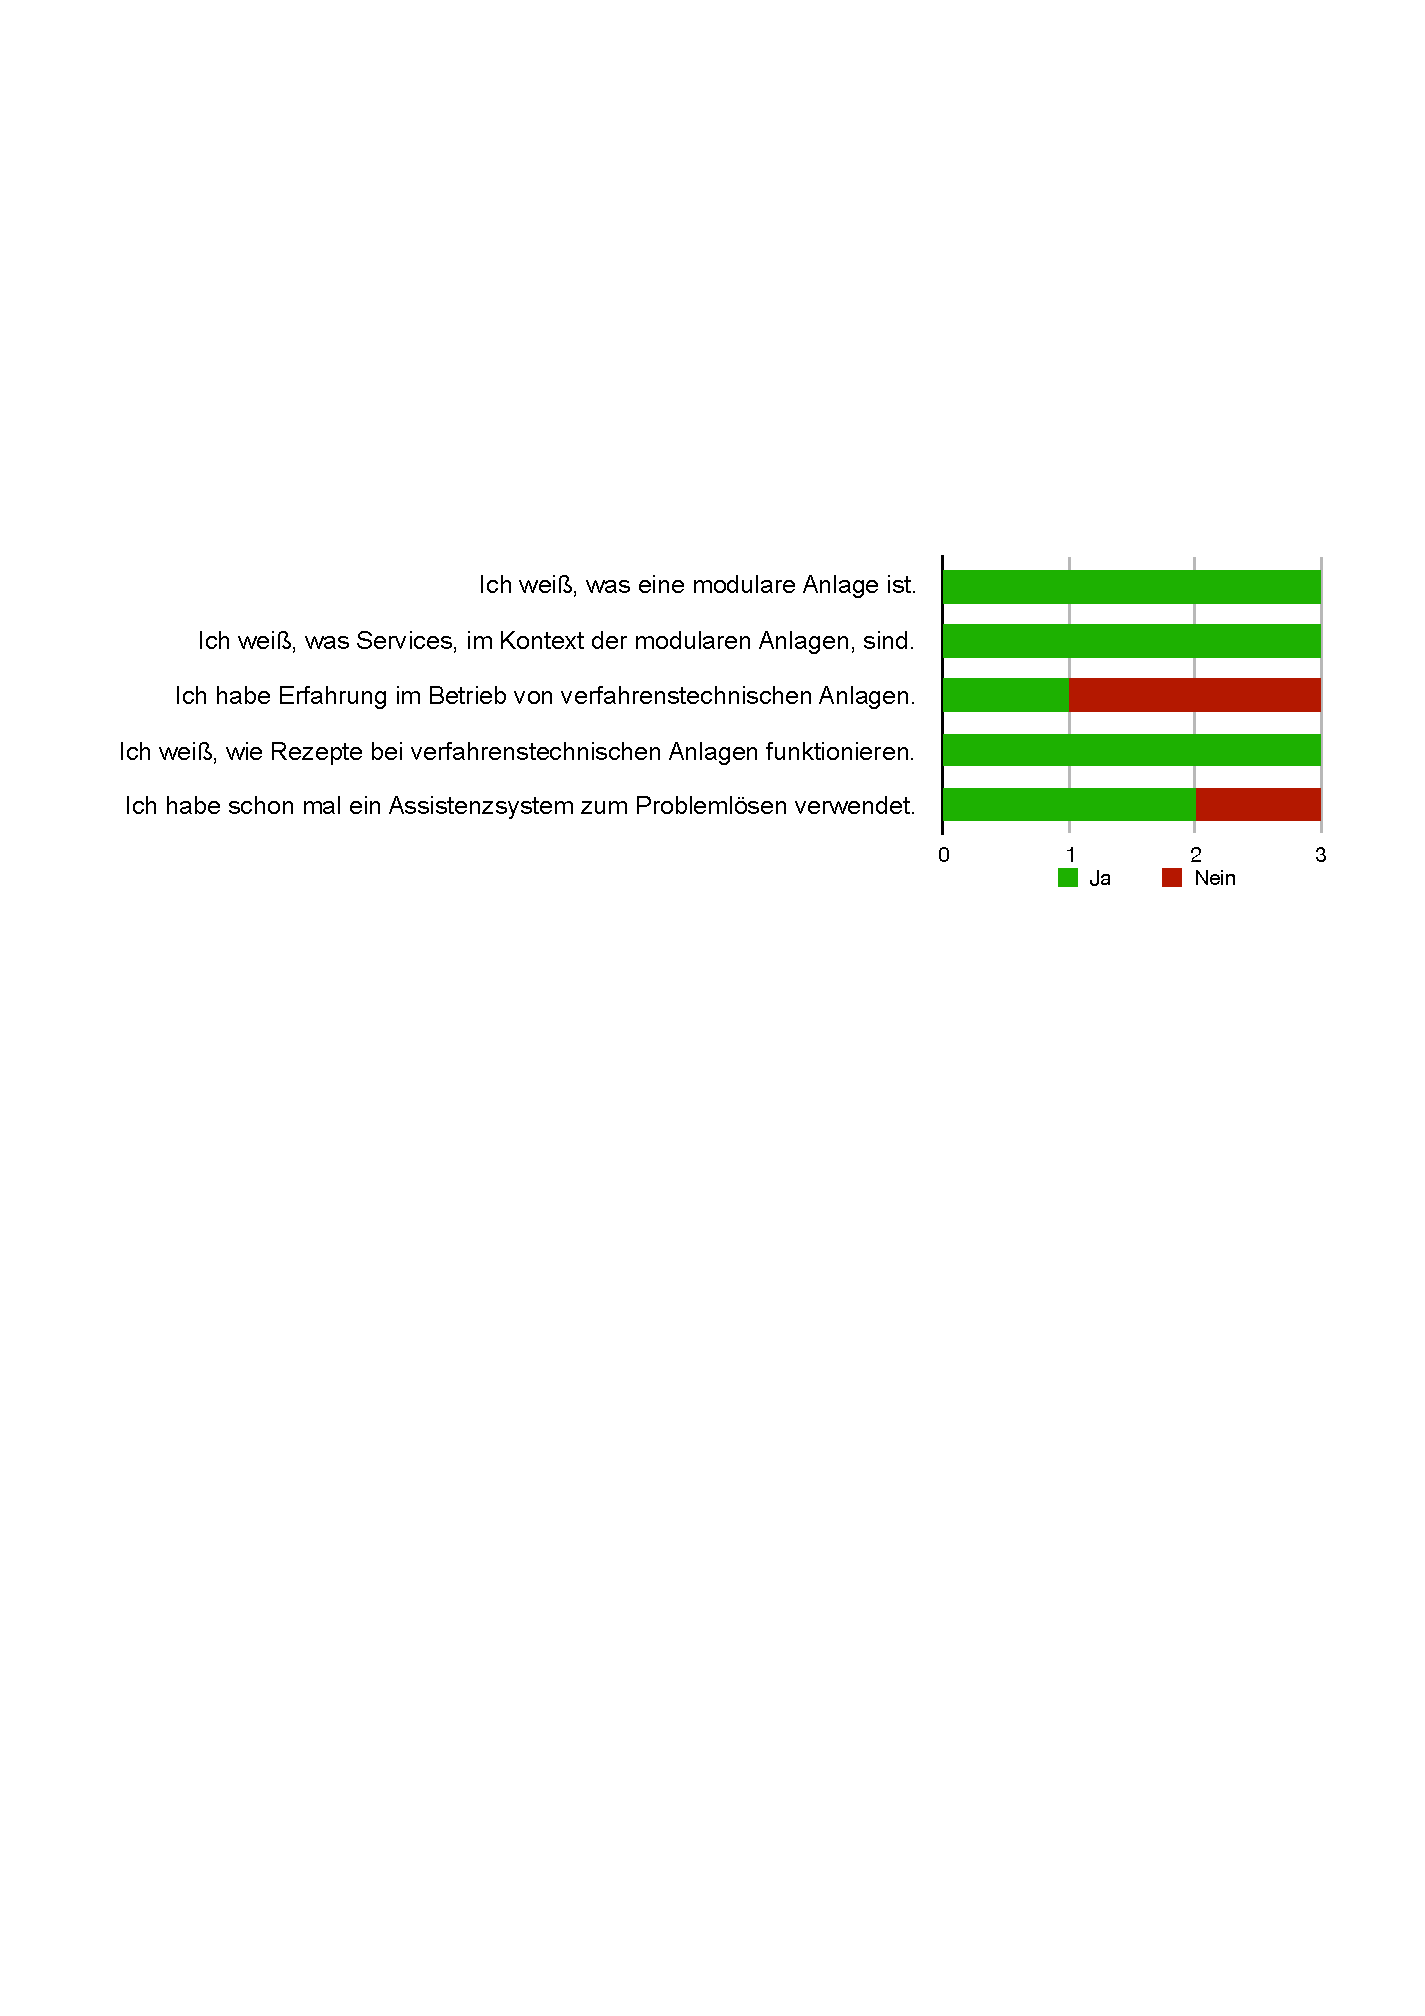
\includegraphics[scale=0.65]{DA_files/Bilder/Validierung/Bild-Vorwissen.pdf}
\caption{Vorwissen zu modularen Anlagen und Assistenzsystemen}
\label{pic:Fragebogen-Vorwissen}
\end{figure}

\begin{figure}[htbp]
\centering

\end{figure}

\subsubsection*{Für gut befunden}
Vorschlag von mehreren Lösungen

Sehr übersichtlich

\subsubsection*{Verbesserungsvorschläge}
Gesamtkosten aufführen -> was kostet ein Mitarbeiter (haben sowohl Luise, als auch Valentin gesagt)

Wunsch: Beim Durchführen der Lösungen unterstützen

Kennt das Assistenzsysteme alle möglichen Lösungen 


\section{Zusammenfassung}
Anforderungen:
Problemidentifikation -> gut erfüllt, es fehlt die Möglichkeit, dass der Nutzer Probleme erstellen kann; noch unklar, welche Informationen das Unternehmen über Produktionsprozess wünscht

Problemlösung -> mäßig erfüllt, da Nutzer keine Lösungen vorschlagen kann, die Auswirkungen auf den Produktionsprozess nicht angezeigt werden (digital Twin)

Klustern

----

Nutzerumfrage
\chapter{Fazit}
\label{Zusammenfassung}
Die Modularisierungskonzepte für die Prozessindustrie erhöhen die Flexibilität bei der Entwicklung von Anlagen. Sie stellen den Nutzer vor die Herausforderung, Probleme nicht mehr auf Grundlage von umfangreicher Erfahrung lösen zu können \cite{Muller2018}.

Für eine geeignete Unterstützung wurde identifiziert, was bei einem Assistenzsystem für modulare Anlagen zu berücksichtigen ist. Darauf aufbauend entstand eine Nutzeroberfläche, die Probleme und Lösungen darstellt. Die Nutzeroberfläche dient zur Kommunikation zwischen Mensch und Assistenz. Die Assistenz analysiert im Hintergrund die vorhandenen Informationen und teilt sie dem Nutzer über die Interaktionsplattform mit. Dadurch entsteht ein kollaborativer Problemlöseprozess. Anhand eines Use Case wurde ein Prototyp entwickelt, der auf den entworfenen Konzepten aufbaut. Mit diesem konnte eine Umfrage unter Experten durchgeführt werden. Die Auswertung der Umfrage zeigt, dass die Nutzeroberfläche, bei Erweiterung um ein intelligentes System, Anwendung findet.

\section{Zusammenfassung}
Assistenzsysteme können den Menschen bei vielen Dingen unterstützen. Die Möglichkeiten reichen von einfachen Hinweisen bis hin zum automatischem Ausführen von Aufgaben \cite{Wandke2005}. Jede Art von Unterstützung fordert eine angemessene Gestaltung. Für den Nutzer ist es wichtig, dass die Verwendung des Assistenzsystems nicht zu Frustration sondern zu Freude, Spaß und Stolz führt \cite{Hassenzahl2008}. Relevant ist das insbesondere mit Blick auf einen komplexen Problemlöseprozess. Dieser wird sowohl durch die Emotionen des Menschen als auch die Art und Menge der bereitgestellten Informationen beeinflusst. 

Bei der Entwicklung eines Assistenzsystems für modulare Anlagen sind einerseits die Informationen, die vom Modul bereit gestellt werden, andererseits die notwendigen Informationen für ein produzierendes Unternehmen zu berücksichtigen. Die bereits entwickelte Prozessführungsebene zeigt nur einen Teil der vorhandenen Informationen an und unterstützt den Nutzer bei auftretenden Problemen nicht. Informationen, die vom Modul bereit gestellt aber nicht angezeigt werden, sind unter anderem Meldungen, Warnung und Alarme, Serviceabhängigkeiten und das zugehörige Equipment der Services. Für eine erfolgreiche Problemlösung müssen die zu erreichenden Ziele klar sein. Diese orientieren sich an den Einflussgrößen in einem produzierenden Unternehmen. Ein Unternehmen besteht aus verschiedene Ebenen \nicetohave{umformulieren}. Auf der Ebene der Produktionsplanung ist unter anderem die Kapazitätsoptimierung relevant, auf die in dieser Arbeit der Schwerpunkt gelegt wurde. Um den Anlagenbediener bei seiner Aufgabe zu unterstützen, findet ein mittlerer Grad an Automatisierung Anwendung. Dies wird laut Sauer und Chavaillaz \cite{Sauer2018} von Anlagenbedienern bevorzugt und generiert die meisten Lösungsvarianten \cite{Miller2005}.

Die entwickelte Nutzeroberfläche begleitet den Nutzer durch die Phasen des Problemlöseprozesses. In Phase eins, der Problemidentifikation, wird auf Meldungen, Warnungen und Alarme aufmerksam gemacht, die ein Problem verursachen. Ein Problem entsteht erst, wenn die Meldungen, Warnungen und Alarme nicht mit den Zielen des Unternehmens vereinbar sind. Das Assistenzsystem identifiziert, welchem Bereich das Problem zugeordnet ist. Es werden die auslösenden Bereiche Modul, KPI, Rezept und Service unterschieden. Entscheidet der Nutzer das Problem zu bearbeiten, geht der Problemlöseprozess in Phase zwei, die Ziel- und Situationsanalyse, über. In dieser hebt das Assistenzsystem hervor, welche Zusammenhänge zwischen Problem und dem Rest der modularen Anlage bestehen. Zusätzlich wird der Nutzer bei der Parametrierung der Ziele unterstützt. Er hat die Möglichkeit, die Parameter der vorgeschlagenen Ziele zu verändern, Ziele hinzuzufügen oder zu löschen. Wenn der Nutzer seine Eingaben bestätigt, folgt Phase drei, die Planerstellung. Dabei sucht das Assistenzsystem nach geeigneten Lösungen, die sich am Problem und den gesetzten Zielen orientieren. Es wird dem Nutzer zum einen angezeigt, welche Elemente (z. B. Services) sich durch Anwendung der Lösung in der modularen Anlage verändern. Zum anderen können in einer tabellarischen Übersicht die Lösungen anhand ihrer Parameter, wie entstehende Kosten und voraussichtlicher Zeitaufwand, verglichen werden. Diese Angaben sollen eine Entscheidung erleichtern.

Die Umfrage unter den Experten ergab, dass die Entscheidung zwar erleichtert wird, sie jedoch immer noch schwierig ist. Sie wünschen sich einheitlich, dass zu der notwendigen Anzahl an Mitarbeitern auch angezeigt wird, welche Kosten ein Mitarbeiter verursacht. Durch Angabe der Gesamtkosten erhoffen sich die Experten eine bessere Vergleichbarkeit der einzelnen Lösungen. Insgesamt wurde der Automatisierungsgrade des Assistenten positiv bewertet. Die Auswahl an Zielen und Lösungen ist, laut der Experten, angemessen, da diese den Nutzer gut leiten. Aufgrund des schlichten Aufbaus, der Übersichtlichkeit und der einfachen Bedienung wird die Nutzeroberfläche von den Experten empfohlen. Für eine konkrete Anwendung der Nutzeroberfläche wird zudem gewünscht, den Nutzer auch bei der Durchführung der Lösung zu unterstützen.

\section{Ausblick}
Diese Arbeit zeigt, dass der Entwurf einen Assistenzsystems für modulare Anlagen vielschichtig ist und von vielen Faktoren beeinflusst wird. Für eine erfolgreiche Anwendung der Nutzeroberfläche sind noch einige Bereiche zu untersuchen. Der Prototyp und auch Teile des Konzepts bauen auf einem konkreten Use Case auf. Das Konzept betrachtet die bestehenden Zusammenhänge zwischen Problemauslöser und Gesamtanlage. Für eine ideale Anpassung an Probleme bleibt zu überprüfen, ob die groben Bereiche Modul, KPI, Rezept und Service ausreichend sind, um den Nutzer ideal zu unterstützen. Mit diesen Informationen kann die Nutzerplattform weiter entwickelt und getestet werden. Bis jetzt ist noch nicht eindeutig, welche Probleme in modularen Anlagen im Detail entstehen bzw. entstehen können.  Eine Möglichkeit wäre, zunächst zwischen anlagen- und modulspezifischen Problemen zu unterscheiden. Um das Problem und die Lösungen geeignet darzustellen, benötigt die Nutzeroberfläche eine ganze Reihe an Informationen. Diese reichen vom Problembereich, über die Ziele bis hin zu den Zusammenhängen. Es bleibt zu untersuchen, wie diese Menge an Informationen vom Modul an die Assistenz und von der Assistenz an die Interaktionsplattform übertragen werden können. Bei der Datenübertragung ist sowohl die Problembeschreibung als auch die Lösungsfindung zu berücksichtigen.

Damit die Assistenz Lösungen finden kann, ist zu klären, welche Daten vom MTP bereitgestellt werden müssen. Dafür sind auch anwendbare Möglichkeiten zur Lösungsfindung zu prüfen. Wenn Lösungen auf vorher bearbeiteten Problemen aufbauen und dies dem Nutzer mitgeteilt wird, könnte er sich leichter für eine Lösung entscheiden und Erfahrungswissen aufbauen. Die entwickelte Nutzeroberfläche kann für eine solche Untersuchung, bei Ergänzung der entsprechenden Information, verwendet werden. Hat der Nutzer und/oder die Assistenz die Möglichkeit, Lösungen vorab an einer virtuell modularen Anlage zu testen, könnten dadurch Fehlentscheidungen reduziert werden. Durch umfassende Analyse der thematisierten Faktoren kann aus der Nutzeroberfläche ein intelligentes Assistenzsystem werden, das dann in modularen Anlagen verwendbar ist.
\chapter{Ausblick}
\label{Ausblick}
Diese Arbeit zeigt, dass der Entwurf einen Assistenzsystems für modulare Anlagen vielschichtig ist und von vielen Faktoren beeinflusst wird. Für eine erfolgreiche Anwendung der Nutzeroberfläche sind noch einige Bereiche zu untersuchen. Der Prototyp und auch Teile des Konzepts bauen auf einem konkreten Use Case auf. Das Konzept betrachtet, welche groben Zusammenhänge zwischen Problemauslöser und Gesamtanlage bestehen. Für eine ideale Anpassung an Probleme bleibt zu überprüfen, ob die groben Bereiche Modul, KPI, Rezept und Service ausreichend sind. Bis jetzt ist noch nicht eindeutig, welche Probleme in modularen Anlagen im Detail entstehen bzw. entstehen können. Mit diesen Informationen kann die Nutzerplattform weiter entwickelt und getestet werden. Eine Möglichkeit wäre, zunächst zwischen anlagen- und modulspezifischen Problemen zu unterscheiden. 

\todo{überarbeiten}
%Diese Arbeit zeigt, dass viele Faktoren den Entwurf eines Assistenzsystems für modulare Anlagen beeinflussen. Für eine erfolgreiche Umsetzung sind noch entsprechend viele Bereich zu untersuchen. Der Prototyp und auch Teile des Konzepts bauen auf einem konkreten Use Case auf. Das Konzept betrachtet, welche groben Zusammenhänge zwischen Problemauslöser und Gesamtanlage bestehen. Damit sich die Interaktionsplattform ideal anpassen kann, muss noch erforscht werden, welche Probleme im Detail entstehen bzw. entstehen könnten und wie sich diese konkret unterscheiden lassen. Eine Möglichkeit ist, zunächst zwischen anlagen- und modulspezifischen Problemen zu unterscheiden. Im Zuge dessen ist auch zu untersuchen, welche Daten vom Modul an die Assistenz und welche Daten von der Assistenz an die Interaktionsplattform übertragen werden müssen. Bei der Datenübertragung ist sowohl die Problembeschreibung als auch die Lösungsfindung zu berücksichtigen. 

Es ist noch nicht geklärt, welche Daten vom MTP bereitgestellt werden müssen, damit die Assistenz Lösungen finden und den Nutzer ideal unterstützen kann. Dafür ist auch zu untersuchen, welche Möglichkeiten zur Lösungsfindung anwendbar sind. Es stellen sich folgende Fragen: Basieren Lösungen auf schon vorher bearbeitenden Problemen? Hat der Nutzer über eine virtuelle modulare Anlagen die Möglichkeit, vorab Lösungen zu testen? Kann die Assistenz die Lösung von ähnlichen Probleme mit der virtuellen Anlage testen, um vorab zu bestimmen, ob es eine sinnvolle Lösung ist? Diese Fragen müssen für die Anwendung der Nutzeroberfläche noch beantwortet werden.
---------------------------------------------

Welche Informationen sind für welche Ziele relevant?

Wie unterscheiden sich Meldungen, Warnungen, Alarme hinsichtlich Zeit, Komplexität? Kann man dort schon Probleme unterscheiden? Welche Informationen müssen übergeben werden?

         
          
\end{document}